\documentclass{pracamgren}

\usepackage[table, svgnames, dvipsnames]{xcolor}

%\usepackage{lmodern}
\usepackage[T1]{fontenc}
%\usepackage{color}
\usepackage{algpseudocode}
\usepackage{algorithm}
\usepackage[framemethod=tikz]{mdframed}
\usepackage{amsmath}
\usepackage{amsfonts}
\usepackage{epsfig}
\usepackage{pstricks}
\usepackage{graphicx}
\usepackage{algorithm}
\usepackage{algpseudocode}
\usepackage[backend=biber,style=authoryear-comp,sorting=nyt,maxcitenames=2,uniquename=false,uniquelist=false,maxbibnames=5,maxsortnames=1]{biblatex}
\usepackage[font=small,labelfont=bf]{caption}
\usepackage[hidelinks,allcolors=black]{hyperref}
\usepackage{upgreek} 
\usepackage{placeins}
\renewcommand{\arraystretch}{1.1}

\setlength{\parskip}{0pt}

\addbibresource{msc-thesis.bib}
\author{Maciej Manna}
\nralbumu{1065745}
\title{Massively Parallel Pseudo-Spectral DNS and~LES for Particle-Laden Turbulent Flows under Two-Way Momentum Coupling}
\tytul{Masywnie równoległe pseudo-spektralne symulacje DNS i LES przepływów turbulentnych z\,cząstkami przy uwzględnieniu dwustronnego sprzężenia pędu}
\kierunek{computer science}
\opiekun{Dr. hab. Bogdan Rosa \\
Warsaw University of Life Sciences -- SGGW \\
Institute of Information Technology; \\
Institute of Meteorology and Water Management \\ National Research Institute
}

\date{September 2022}

\dziedzina{11.3 Informatyka\\}
\dziedzinaang{11.3 Informatics, Computer Science\\}

\keywords{obliczeniowa mechanika płynów, przepływ turbulentny, przepływ wielofazowy, krople, mikrofizyka chmur, obliczenia dużej mocy, równania Naviera-Stokesa, homogeniczna izotropowa turbulencja, statystyki zderzeniowe kropel, metoda pseudo-spektralna, bezpośrednia symulacja numeryczna (DNS), metoda dużych wirów (LES), dwustronne sprzeżenie pędu, efekty grawitacyjne}
\keywordsang{computational fluid mechanics, turbulent flow, multiphase flow, droplets, cloud microphysics, high performance computing, Navier-Stokes equations, homogeneous isotropic turbulence, droplet collision statistics, pseudo-spectral method, direct numerical simulation, large-eddy simulation, two-way momentum coupling, gravitational effects}




\begin{document}
\maketitle

\streszczenie{
Przepływy turbulentne z cząstkami fazy rozproszonej zachodzą nieustannie w środowisku naturalnym oraz znajdują liczne zastosowania w procesach przemysłowych.
Ważnym tego przykładem są chmury atmosferyczne, które składają się z ogromnej ilości małych kropel wody i kryształków lodu.
Wyjaśnienie wzajemnego oddziaływania powietrza (płynu) i aerozolu (cząstek) jest istotne w kontekście poznania mechanizmów rządzących powstawaniem i przebiegiem zjawisk atmosferycznych.
Wiedza w tym zakresie jest użyteczna w obszarze meteorologii i służy do opracowywania coraz to bardziej realistycznych modeli powstawania opadu z kropel chmurowych.
To z kolei prowadzi do podniesienia dokładności i sprawdzalności numerycznych prognoz pogody.
Jednym ze sposobów badania przepływów dyspersyjnych są symulacje numeryczne. 
\newline \indent
Powszechnie stosowanym do tego celu narzędziem, zapewniającym wysoką dokładność, są tzw. bezpośrednie symulacje numeryczne (direct numerical simulation, DNS). 
Za pomocą symulacji DNS można pozyskiwać statystyki zderzeniowe cząstek, które to są użyteczne jako parametry w modelach obejmujących większe skale przestrzenne.
Symulacje DNS są~jednak kosztowne obliczeniowo, co ogranicza ich stosowalność do siatek o średnich rozmiarach (${\sim 2048^3}$ węzłów - przy współcześnie dostępnych zasobach obliczeniowych).
DNS nie pozwalają modelować turbulencji charakteryzowanej wyższymi liczbami Reynoldsa ($R_{\lambda} \sim 10^4$), czyli takiej która obserwowana jest w powietrzu atmosferycznym. \newline \indent
Metoda dużych wirów (large-eddy simulation, LES) stanowi alternatywę dla DNS.
W tej metodzie drobnoskalowa turbulencja nie jest bezpośrednio rozwiązywana, ale jest parametryzowana przy użyciu modelu podskalowego.
Umożliwia to modelowanie przepływów turbulentnych o większej liczbie Reynoldsa przy użyciu siatek o mniejszej liczbie węzłów.
Ograniczenie złożoności obliczeniowej odbywa się jednak kosztem mniejszej precyzji i fizycznej dokładności.
Niniejsza praca stanowi porównanie obu metod (DNS i LES), zarówno w kwestii fizycznej dokładności, jak i wydajności, skupiając się w szczególności na symulacjach z dwustronnym sprzężeniem pędu pomiędzy płynem i cząstkami. 
Zostało wykazane, że LES stanowi obiecującą odpowiedź na ograniczenia DNSu, pomimo pewnych niedokładności wynikających z filtrowania turbulencji w najmniejszych skalach.
Różnice te, w większości przypadków, stają się mniejsze, gdy uwzględni się dwustronne sprzężenie pędu, w szczególności dla cząstek poddanych działaniu grawitacji.
\newline \indent
Przeprowadzone zostały również analizy kosztów obliczeniowych obu metod.
Choć zastosowanie LES zapewnia ogromną oszczędność w obliczeniach związanych z turbulentnym przepływem płynu, to jednak koszt ten znacząco rośnie wraz z liczbą cząstek.
Niezbędna ilość symulowanych cząstek może zaś być duża, gdyż efekty dwustronnego sprzężenia pędu objawiają się wyraźniej w układach z względnie wysokim stosunkiem masy cząstek i płynu (pomiędzy $0.1$~i~$1$).
Zatem obliczenia odnoszące się do dynamiki cząstek stanowią bardziej istotne ograniczenie dla LESu niż dla DNSu, gdzie złożoność obliczeń związanych z~płynem jest czynnikiem dominującym.
Ponadto zidentyfikowano i przeanalizowano szereg parametrów, które pośrednio wpływają na czas trwania symulacji, takie jak np. promienie kropel oraz~działanie grawitacji.
Na~koniec przedstawiono także wpływ preferencyjnego koncentrowania się cząstek na wariancję ich rozkładu pomiędzy równolegle wykonywanymi procesami.
Ten czynnik ma~również istotne znaczenie w kontekście całkowitej wydajności symulacji.
}

\renewcommand{\abstractname}{Abstract}
\begin{abstract}
Turbulent fluid flows with dispersed particles are a common occurrence in nature, as~well~as in many technological processes.
An important example of such systems are atmospheric clouds that consist of a huge number of small water droplets and ice crystals suspended in air.
The~understanding of interplay between air (fluid) and aerosol (particles) is crucial for increasing the accuracy and reliability of numerical weather forecasts through more realistic modelling of atmospheric phenomena.
Performing numerical simulations on a fine scale is one way of studying such processes.

Direct numerical simulations (DNS) prove to be a relatively precise tool that is widely used in these studies.
DNS can be used to obtain the particle collision statistics obtained from these simulations may be further utilised as parameterisations for larger-scale models.
These simulations, however, are costly in terms of computational complexity, hence their application is limited to moderate-sized grids ($\sim 2048^3$ nodes, with the computing power of modern supercomputers).
For that reason DNS are not able to resolve turbulence characterised by~higher Reynolds numbers ($R_{\lambda} \sim 10^4$), which is observed in atmospheric air.  

Large-eddy simulations (LES) provide an alternative approach to DNS.
In this method small-scale turbulence is not directly resolved but parameterised using a subgrid-scale model.
This reduces the grid size required to achieve higher Reynolds numbers (and, thus, computational complexity) at the cost of diminished precision and physical fidelity. 
This thesis provides comparison of DNS and LES, both in terms of physical fidelity and performance, focusing primarily on simulations under two-way momentum coupling between the fluid and particles.
LES is shown to be a promising solution to limitations of DNS, even though it~exhibits certain inaccuracies that may be attributed to the filtering of small-scale vortical structures.
These discrepancies, for the most part, become less pronounced when two-way momentum coupling is considered, especially for settling particles.

Furthermore, a broader study of computational costs for both methods is presented.
Even~though LES provides immense performance advantage when it comes to fluid simulation, it~is~highly susceptible to the growing number of individually tracked particles.
The amount of particles that are needed may be considerable, as effects of two-way momentum coupling manifest when particle mass loadings are relatively high (between $0.1$ and $1$).
Thus, computations related to particles are recognised to be a much more significant bottleneck for~LES than for DNS, where the complexity of fluid simulation is the largest concern.
In~addition, several parameters that indirectly influence the execution time are identified and analysed, such as droplet radii or effects of gravity.
Finally, it is shown that the preferential concentration of particles may affect the variance of their distribution between parallel processes and~consequently influence the overall simulation performance.
 
\end{abstract}


\tableofcontents


\chapter*{Acknowledgements}
\addcontentsline{toc}{chapter}{\numberline{}Acknowledgements}
\label{ch:ack}

\textbf{This thesis was created as part of a project: \emph{Turbulent flow analysis with~the~dispersion phase - the impact of two-sided coupling of momentum and gravity on~particle motion statistics} of National Science Centre (NCN) -- OPUS14/2017, project no.: \emph{UMO-2017/27/B/ST8/00555}.}

\smallskip
\noindent 
\textbf{The access to computational resources and supercomputer \emph{Okeanos} used to obtain results presented in this thesis was provided by Interdisciplinary Centre for Mathematical and Computational Modelling (ICM) at Warsaw University (grants: GA73-14, GA84-22, and G87-1145)}.

\bigskip

First and foremost, I would like to thank the supervisor of this thesis, as well as grants~mentioned above, Dr. hab. Bogdan Rosa (Warsaw University of Life Sciences -- SGGW, Warsaw; Institute of Meteorology and Water Management -- National Research Institute, Warsaw), for~excellent introduction and guidance in the subject matter of the thesis, as~well~as continuous encouragement and understanding during the process of its creation.
I would also like to express my gratitude to Dr. Sylwester Arabas (Jagiellonian University, Kraków), who introduced me to the modelling of atmospheric cloud and supported in pursuing further involvement in that field, for his valuable comments, as well as aid in administrative affairs.
Furthermore, I~would like to acknowledge all creators, maintainers, and developers of~the~pseudo-spectral solver code, especially Prof. Lian-Ping Wang (University of Delaware; currently Southern University of Science and Technology, Shenzhen) and Dr.~hab.~Bogdan Rosa, as well as the copyright holder, University of Delaware, for permission to use and modify it~in~order to obtain results presented in this thesis.
Finally, I~would like to thank Prof. Jacek Pozorski (Institute of Fluid Flow Machinery, Polish Academy of Sciences, Gdańsk), as well as all participants of A2S Group Seminar (AGH University of~Science and Technology, Kraków) and Seminar on Partial Differential Equations (Jagiellonian University, Kraków) for~valuable questions and discussions that helped in shaping the final draft of this thesis. 


\chapter*{Introduction}
\addcontentsline{toc}{chapter}{\numberline{}Introduction}
\label{ch:int}


\emph{Turbulence} is the phenomenon that accompanies most of the real-world situations where fluid flows are encountered.
Distinction between \emph{laminar} and \emph{turbulent flows} is very practical, as~the~former represents much more organised, layered, and stable fluid motion that is easier to analyse and quantify, while the latter is inherently irregular, and its parameters have~to~be~approached statistically.
Turbulence gives rise to eddies that span wide range of~spatial and temporal scales where different dynamical properties of the fluid are most pronounced.
We commonly distinguish three subranges in the entire span of eddy sizes.
There is \emph{integral length scale} that includes largest eddies containing most of the energy of~a~system.
Then, we consider \emph{inertial subrange}, where turbulence kinetic energy is transferred from larger eddies to the smaller ones in a process referred to as the \emph{energy cascade}.
Finally, we have subrange that consists of smallest eddy sizes, the so-called \emph{Kolmogorov microscale}, where influence of fluid viscosity is paramount, and where the kinetic energy of slowly vanishing eddies is dissipated into heat.
Such complex behaviour arises due to the nonlinearity of~equations governing the fluid motion, which makes turbulent flows famously difficult to~study analytically.
Hence, numeric simulations are often employed to model and study these physical phenomena.

Many processes that involve fluid flows, whether laminar or turbulent, are composed of~more than one phase.
Here, by \emph{phase}, we understand regions of the system with the same properties that can be clearly separated by some interface from others.
We refer to~such flows as \emph{multi-phase}, or \emph{two-phase}, in a common case where the number of considered phases is~limited to two.
These phases often are of different states of matter, e.g. gas--liquid for air bubbles flowing in the water pipe, but systems with two immiscible liquids, such as water and crude oil in pipelines, are also studied \parencite{Brauner2003}.
In many cases, one of the phases may be~treated as continuous (referred to as the \emph{continuous phase}, or the \emph{carrier fluid}), while the other (either dispersed fluid, or any other particulate matter) remains in~separated chunks.
Then, we refer to such chunks as the \emph{disperse phase}, and examples may include air bubbles, water droplets, solid particulate matter suspended in a fluid, etc.
Often enough, elements of~disperse phase may be approximated as \emph{point particles}, i.e. material points that are conceptually representing small spheres of given radii, that are considered insoluble and immiscible (that is, they cannot exchange mass with the carrier fluid, suddenly appear, or~be~destroyed).
Such approximation is especially accurate when disperse phase consists of~small droplets or~bubbles of one fluid surrounded by another, as the surface tension naturally preserves spherical shape of disperse elements.
Cloud droplets, in particular, remain spherical since the capillary pressure is several orders of magnitude larger than the local fluid shear stress induced by~the~disturbance flow associated with their motion.
Furthermore, \textcite[Figure 1, therein]{Balachandar2010} point out that for such approximation to be valid, particle response times have to be greater than Kolmogorov time scale of background turbulent flow. 
We shall refer to two-phase flows with disperse phase approximated by point particles as \emph{particle-laden}.

The modelling of flows that both exhibit turbulent behaviour and include population of~particles interacting with that flow gives rise to even more complexity.
As stated by \textcite{Balachandar2010}, ``turbulence and multiphase flows are two of the most challenging topics in fluid mechanics, and when combined they pose a formidable challenge, even in~the~dilute dispersed regime''.
In spite of that, the number and importance of real-life applications that involve such systems is quite significant, and more than justifies development of effective methods in that domain.
To mention just a few, we may consider some technological, and industrial applications, such as analysis of combustion of liquid fuel aerosols in engines or combustion of pulverised coal in furnaces \parencite{Zheng2020}, as well as other technologies, including fluidised beds, transport systems, and pollution control \parencite[4-17]{Crowe2012}.
Such systems are also studied in ecology (e.g. transport of pollutants in the atmosphere or sediments in water) and agriculture (efficient spraying of fertilisers).
Finally, the modelling of atmospheric clouds, that essentially are huge collections of small water droplets and ice crystals suspended in often turbulent air, is the backbone of all meteorological and climate science models used for analysis and prediction \parencite{Devenish2012, Grabowski2013}.
In this thesis we shall focus our study of particle-laden turbulent flows on applications in cloud modelling, but general methods presented here are not limited to that particular use case.

The modelling of atmospheric clouds is a broad domain that has to deal with wide range of~length scales, where different structures and physical processes are important and~have to~be~directly represented, while others need to be parameterised due to constraints in computing power.
Such tradeoff between computational complexity and physical fidelity of simulations gives rise to the plethora of methods used depending on respective scale.
Simplified picture of that situation is presented in Figure \ref{fig:atmo-scales}.
At the largest scales we have \emph{global climate models} (GCM) and \emph{global weather models} (GWM, e.g. Integrated Forecasting System, Global Forecasting Systems, ICON), where computation domain  often spans the entire Earth ($\sim 10^{7}$~m) and each cell has (horizontal) dimensions ranging from $10$ to $100$ kilometres.
We~also~consider \emph{mesoscale models} that are mainly used for weather prediction in smaller domains that usually cover regions, countries, or continents ($\sim 10^{5} \text{--} 10^{6}$ m) and grid spacing is in the order of kilometres.
For instance, maximal resolution of mesoscale model COSMO used for weather forecasting in Poland is $2.8$ km \parencite{Doms2021}.
In this context it~is~worth adding that a small cloud with a volume of $1 \; \text{km}^3$ may have $10^{17}$ drops or more.
Both types of models, due to relatively large grid cell sizes, cannot fully resolve even fairly large cloud structures and depend on a lot of parameterisations.
In the middle ground, we~have~\emph{cloud resolving models} (CRM; domain sizes---kilometres, cell sizes---metres) that cannot fully resolve all turbulent scales of air or exactly model behaviour of every droplet, thus necessary parameterisations are employed, such as large-eddy simulations (LES) and super-droplet method \parencite{Arabas2013}.
CRM is commonly employed for research studies focused on effects of microphysical processes affecting entire clouds, their formation and evolution, precipitation, etc.
For that reason, CRMs are used to refine cloud parameterisations used in GCM and mesoscale models.

\begin{figure}[h]
\centering
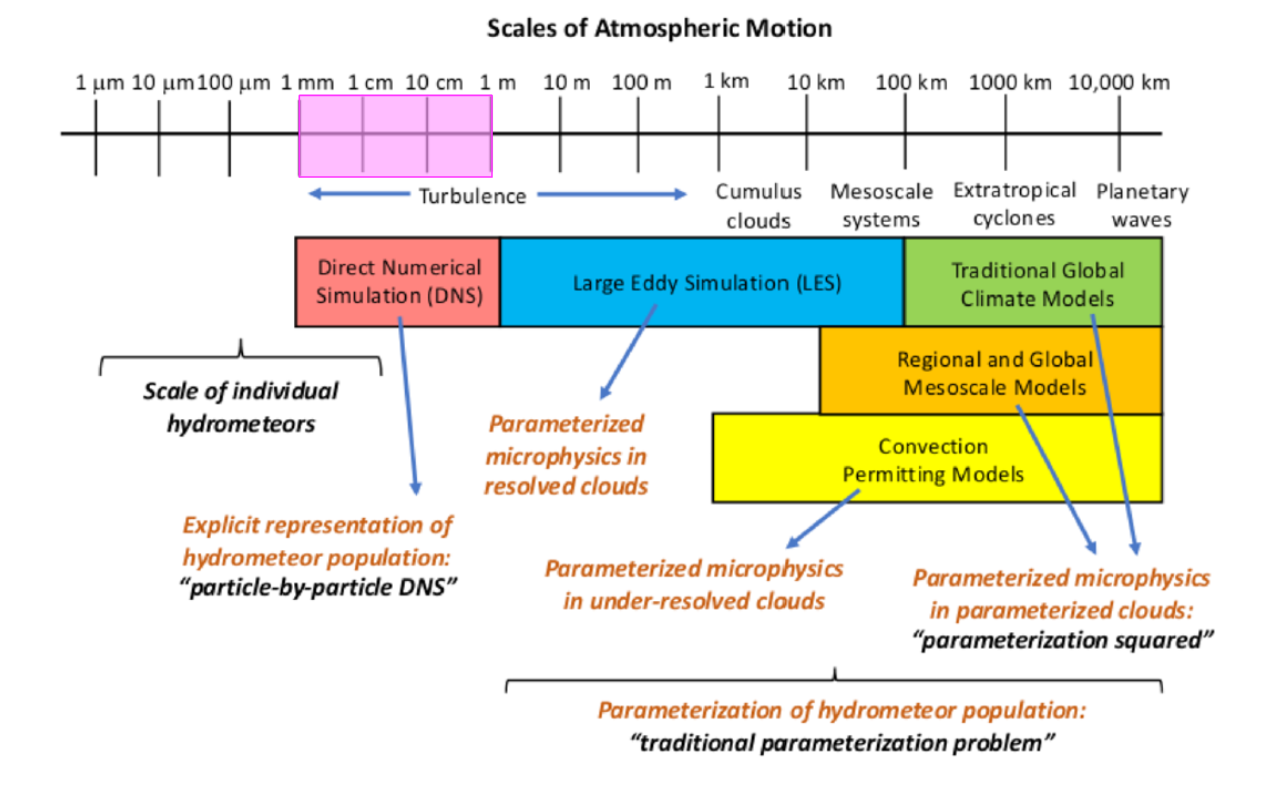
\includegraphics[width=13cm]{img/figs/atmo-scales.png}
\caption{
Hierarchy of atmospheric models and the scales of atmospheric motion reproduced from~\textcite{Morrison2020} with author's permission.
Coloured rectangles represent types of simulations commonly used when working with respective length scales, and comments emphasise transition from~directly resolving most elements of the model (left) to including more and more parameterisations with increase of scale (right).
Magenta rectangle positioned on the axis was added to emphasise range of scales that corresponds to simulations discussed in this thesis.
}
\label{fig:atmo-scales}
\end{figure}

Finally, we enter scales where point-particle \emph{direct numerical simulations} (DNS) can~be~used to~obtain more precise picture of small-scale turbulent phenomena that affect cloud microphysics.
These methods allow direct resolution of wide range of turbulent scales, including Kolmogorov microscales, which are estimated to be of the order of 1 mm in Earth's atmosphere.
Also, all particles (droplets) are individually tracked, so that their dynamics and~interaction with carrier flow may be directly computed (note, that $1 \, \text{m}^{3}$ of cloudy volume contains, approximately, up to $10^{8}$ droplets).
Due to small sizes of grid cells required to~resolve even the smallest eddies, as well as considerable computational demand of handling large numbers of particles, point-particle DNS are limited to volumes of about $1 \, \text{m}^{3}$ \parencite{Morrison2020}.

Despite these limitations, however, such simulations provide essential backbone to entire hierarchy of models by allowing to study small-scale cloud phenomena and estimate parameters used in cloud resolving models (CRM).
One example of such parameter is the \emph{collision kernel} that determines rates of collision between droplets of the same or different sizes, and~it~greatly affects process of droplet growth due to coalescence that is crucial for accurate modelling of precipitation.
Such small domains also justify modelling air turbulence as~homogeneous and isotropic.
Even though energy-containing large-scale eddies in atmosphere generate large-scale inhomogeneity and anisotropy, dissipative small-scale eddies work to flatten the inhomogeneities, leading to local homogeneity and isotropy.
This local homogeneity assumption is the basis of most turbulence models \parencite{Matsuda2021}.

There is, however, another important axis which exhibits similar complexity--fidelity tradeoff, and it pertains to the precision of modelling interactions between particles and carrier fluid.
We use Lagrangian approach to track particles, since time microscales associated with~the~energy dissipation of atmospheric flows and response times of cloud droplets are~usually of~the~same order (i.e. Stokes number, $St$, is close to $1$, see \cite{Balachandar2009}).
The~modelling of~interaction between fluid and particle, however, may be limited to \emph{one-way momentum coupling} (OWC), i.e. particles are transported by the fluid but do not affect its velocity field.
This~simplification is valid for dilute systems, where ratio of total mass of~particles to total mass of fluid (referred to as the particle \emph{mass loading}, $\Phi_m$, of the system) is~small, usually assumed to~be~less than $0.1$ (i.e. less than $0.01\%$ by volume for water droplets in air).
On the other hand, experiments have shown that presence of particles alters statistics of the carrier fluid flow, e.g. suppresses or enhances the turbulence flow depending on the sizes of particles \parencite{Gore1989}.
Also, recent simulation studies \parencite{Rosa2020} have shown that inclusion of momentum transfer in the other direction, i.e. \emph{two-way~momentum coupling} (TWC), provide more complete and complex picture of system dynamics, and~increase physical fidelity of obtained results, even for relatively dilute systems.
Hence, TWC approach is used here, building upon methods and results from \textcite{Rosa2020,Rosa2022}.
Note, that for~very dense systems ($\Phi_m > 1$) it is preferable to also include effects of collisions between particles (four-way momentum coupling), but such conditions are not applicable when considering Earth's atmospheric clouds.
Also, in this context, it is worth to~mention alternative methods for modelling interactions between particles, such as simplified representation of~many-body aerodynamic interactions \parencite[Hybrid DNS, see][]{Wang2009, Ayala2007}), or inclusion of lubrication forces \parencite{Ababaei2021}, however these approaches are~beyond the scope of this study.

\smallskip

In this thesis, small-scale simulations of turbulent, particle-laden flows for the purpose of~obtaining particle collision statistics, such as previously mentioned collision kernels, are~considered.
The domain in question is small enough that we can employ direct numerical simulations for the modelling of homogeneous isotropic turbulence (HIT).
For simplicity, the domain is assumed to be box-shaped and divided into cubic cells uniformly in each dimension.
Also, periodic boundary conditions are imposed on the domain walls.
As introduced above, the~default method applicable for such experiments is point-particle DNS.

Recent studies, however, have shown that direct numerical simulations are close to its limits due to prohibitively large computational costs.
\textcite{Rosa2013,Rosa2016} used grids of~up~to $1024^3$ nodes, which seems to be the reasonable limit for most studies, although there~were studies using even larger grids (e.g. $2048^3$ nodes in \textcite{Ireland2016} and \textcite{Matsuda2021}; for flows without particles grids of size up to $8192^3$ were used by \textcite{Buaria2019}), and more recently even $12\,288^{3}$ \parencite{Buaria2020}.
It is important to note, that grid size is crucial for turbulent flow simulations, since it affects the range of spatial scales that can be resolved, from the smallest eddies with sizes close to the spatial grid spacing, to the largest ones of sizes typically about $1/3$ of the computational domain (this limitation is~due to a numerical requirement that the correlation of fluid velocity at distances comparable to the domain size must vanish).
Such range between largest and smallest resolvable scales can be expressed using \emph{Reynolds number}, which is also commonly interpreted as a measure of~magnitude of~turbuence.
Examples of values of Taylor microscale (that is, considering only eddies in inertial subrange) Reynolds number, $R_{\lambda}$, attained in previous high-resolution studies are $R_{\lambda} = 499$ for $1024^3$ grid \parencite{Rosa2013,Rosa2016}, $R_{\lambda} = 597$ \parencite{Ireland2016}, and $R_{\lambda} = 531$ \parencite{Matsuda2021} for $2048^3$ grids, $R_{\lambda} = 650$ for $8192^3$ \parencite{Buaria2019}, and $R_{\lambda} = 1300$ for $12\,288^3$ grid.
It is desirable, however, to attain higher values of $R_{\lambda}$ to simulate conditions that are present in typical atmospheric clouds, where $R_{\lambda}$~is known to attain values between $10^{3}$ and $10^{4}$.
What is more, the increase of the Taylor microscale Reynolds number with the number of grid nodes in one dimension, $N$, is sublinear (comparison of simulation data from various studies shows that $R_{\lambda} \propto N^{2/3}$, see \cite{Wang2009}, Figure 1, which agree with theoretical estimates for pseudo-spectral method in \cite{Pope2000}, Equation 9.8).
Thus, when we double $N$ we only increase $R_{\lambda}$ by at most $50\% \text{--} 60\%$, while total number of grid nodes, $N^3$, increases by the factor of $8$.
The strategy of increasing grid sizes of~DNS to~model somewhat wider range of turbulent scales currently faces not only resource limitations, but is~also hindered by the diminishing returns in the long run.
This situation calls for~alternative solution.

\emph{Large-eddy simulation} (LES) is a well-developed method that is commonly used when dealing with length scales characteristic to CRM simulations \parencite{Guichard2017}.
Its purpose is to allow modelling of highly turbulent environments in larger domains, where directly resolving smallest eddies is infeasible.
The general idea is to directly resolve larger eddies, as in DNS, but replace direct resolution of the smallest, dissipative turbulent scales with parameterised model, referred to as the \emph{subgrid-scale model}.
This way we may use smaller grid sizes relative to DNS, yet still obtain comparable statistics of turbulent flow, including the Reynolds number.

LES focuses on directly resolving larger scales of turbulence since they contain most of~the~energy of the system, and are most effective transporters of conserved properties (\cite[367]{Ferziger2020}; \cite[352]{Pope2000}).
This property is paramount for CRM, but when using simulations to study small-scale phenomena such strategy is not as easily transferable.
Also, it was repeatedly shown that relative motion and preferential concentration of low-inertia particles is governed mainly by small turbulent structures.
Consequently, the collision-coalescence depends on scales of motion that belong to the dissipation subrange of the energy spectrum.
The interest in applying LES method in small-scale experiments used to estimate particle statistics may be limited, but is growing in recent decades \parencite{Fede2006, Jin2010, Rosa2017}, but no comparable studies that also include effects of TWC were performed.
Therefore, is called for to investigate feasibility of~LES in~that~context, and this thesis aims at providing good starting point for such analyses.

\medskip

The first systematic study using direct numerical simulations of homogeneous and isotropic turbulence with non-settling particles (i.e. unaffected by gravity) under two-way momentum coupling was performed more than thirty years ago by \textcite{Squires1990}.
It focused on the effects that particles have on carrier flow, especially the modulation of turbulence and changes in energy and dissipation spectra due to varying particle mass loadings.
Their~simulations, due to contemporaneous hardware limitations, used small grid sizes ($32^3$ and $64^3$) and thus were limited to $R_{\lambda} = 38$.
In a follow-up study by \textcite{Elghobashi1993} the effect of gravitational settling was considered but the simulations were limited to decaying turbulence.
Other early studies, such as \textcite{Wang1993} and \textcite{Yang1998}, expanded these results to larger meshes but were limited to the one-way momentum~coupling.
More importantly, the latter study \parencite{Yang1998} proposed to use large-eddy simulations to achieve higher $R_{\lambda}$ without going beyond hardware limitations.

These earlier studies, however, did not explicitly consider collisional statistics of particles, such as collision kernels, which are main focus of this thesis.
One of the first systematic studies aimed at estimating these parameters using DNS with homogeneous isotropic turbulence model was \textcite{Ayala2008}, and it was motivated by growing interest in the process of~droplet growth due to collision-coalescence.
Their simulations included effects of gravity and were performed at different values of the energy dissipation rate.
In another study by~\textcite{Wang2008} the main focus was also on collision statistics, but also hydrodynamic interaction between droplets was considered by employing an original method elaborated by \textcite{Ayala2007}.
In both cases, no influence of particles on the fluid flow was taken into account (as~in~TWC), but their method attempted to model hydrodynamic interactions between particles instead.
An example of earlier TWC study that focused on  particle statistics may be the work of \textcite{Bosse2006}, that shows significant enhancement in the mean settling velocity when two-way coupling is considered. 
Later, these results were extended by \textcite{Monchaux2017} for wider ranges of particle volume loadings, also reporting decrease in particle preferential concentration with increasing mass loading.

Two important features of further studies, at least from the point of view of this thesis, are: (1) inclusion of two-way momentum coupling between fluid and particles, and (2) use of large-eddy simulations in that context.
Most of these, however, used only direct numerical simulations that were limited to one-way momentum coupling.
\textcite{Rosa2013} provides results from simulations spanning wide range of grid sizes (from $N=32$ to $N=1024$), and shows, in practice, diminishing growth of $R_{\lambda}$ with respect to $N$.
It also analysed the influence of different forcing schemes on the estimated particle statistics.
Further studies by \textcite{Onishi2013} and \textcite{Ireland2016} are notable because of relatively large grids used that allowed to obtain higher values of $R_{\lambda}$ ($N=2048$ with $R_{\lambda}=597$, and $N=2000$ with $R_{\lambda} = 527$, respectively).
Work by \textcite{Onishi2013} is also worth mentioning, as~instead of pseudo-spectral method it uses finite-difference method, which is considered to be easier to parallelise and adapt to multiprocessor machines.
On that note, of some interest are also recent papers that use Lattice Boltzmann Method to solve underlying homogeneous and isotropic turbulent flow populated by particles tracked using Lagrangian approach \parencite{Ernst2019,Lain2020}.
These studies, however, used only grids of size $128^3$ and since working with highly turbulent flows was not their goal.
They were limited to $R_{\lambda} = 20$.
More recent study of~\textcite{Matsuda2021} is notable for used grid sizes (up to $2048^3$) and~impressive number of particles tracked (up to $1$ billion), as well as interesting measurements of scale-dependent flatness and skewness of particle distribution fields based on wavelets.
Still, these experiments were limited to one-way momentum coupling.

Nonetheless, as already mentioned, it was recent study of \textcite{Rosa2020} that systematically analysed the effects of including two-way momentum coupling on basic statistics of~the~carrier flow, as well as collision statistics of particles.
Their results show that using TWC significantly affects particle statistics that measure clustering, radial relative velocities, and collision rates, as well as dependence of these statistics on the particle mass loading.
These results were recently complemented by \textcite{Rosa2022}, where simulations covering broader range of grid sizes were performed (up to $1024^3$), and the influence of TWC on average settling velocity of particles was explored as well. 
Still, both of those studies were limited to DNS method only.

On the other hand, first systematic study of using LES method for simulating steady homogeneous isotropic turbulence for carrier fluid in particle-laden systems was performed by~\textcite{Fede2006}.
Simulations were performed using finite-volume method on~grids with $128^3$ nodes.
Their effort was focused on measuring influence of subgid-scale modelling on~the~behaviour of heavy inertial particles at collision distances.
In particular, they established that using LES significantly affects particle concentration and collision statistics, as~they depend on small-scale motion of carrier fluid.
Their analysis was limited to non-settling particles.
\textcite{Marchioli2008} arrived at similar conclusions, i.e. that filtering~velocity field at~small-scales leads to inaccuracies in representation of particle segregation and accumulation phenomena, in simulations involving wall-bounded flows.
Meanwhile, \textcite{Yang2008} showed that for different particle statistics, such as longtime single-particle dispersion, some effects of LES parameterisation cancel each other, leading to accurate predictions.
More in depth study on the influence of subgrid-scale modelling on preferential concentration of particles, where principal requirements for such models were established, was proposed by \textcite{Pozorski2009}.

Important comprehensive study of impact of subgrid-scale modelling on particle collision statistics in HIT was performed by \textcite{Jin2010}.
They used the pseudo-spectral method for~the fluid flow calculations and their realisation of LES (i.e. using spectral eddy viscosity model) matches numerical method used in this thesis.
Their results confirmed adverse effect of~LES on the accuracy particle-pair statistics, and established relation between Stokes number, $St$, and sensitivity of these statistics to subgrid-scale modelling.
They concluded that such effects are most noticeable when $St < 3$.
This study involved only non-settling particles, but it was later complemented by \textcite{Rosa2017}, that used the same numerical setup, but focused on particles affected by gravity.
Their results confirmed previous conclusions regarding limitations of LES to properly represent collisional statistics, such as radial distribution function or radial relative velocity.
They also established influence of subgrid-scale modelling on seemingly single-particle statistics, such as average settling velocity.
All studies mentioned above were limited to one-way momentum coupling.

\smallskip

The natural continuation of aforementioned studies is to analyse the influence of both such extensions applied together in the same simulations.
Thus, more precisely, the topic of this thesis regards simulations of homogeneous isotropic turbulence with inertial particles under two-way momentum coupling, both with and without effects of gravity, for the purpose of~estimating their collisional statistics.
Also effects of particles on basic flow statistics shall be discussed.
Both direct numerical simulations (DNS) and large-eddy simulations (LES) are~used to obtain results, providing grounds for comparison of both methods.
To the knowledge of the author, it is the first study in this context, where TWC LES simulations are considered.
For the sake of simplicity, all simulations performed as part of this study will use single, moderately-sized grid of $256^3$ nodes for DNS, and $64^3$ for LES, as in \textcite{Jin2010} and~\textcite{Rosa2017}.
This study aims to fit into much broader and pressing issue of computational limits that are faced by DNS, and establishment of LES as an alternative that opens way to more faithful modelling of atmospheric turbulence.

\smallskip

The comparison between DNS and LES is carried out in two following aspects.

Firstly, the accuracy, or physical fidelity, of LES is analysed.
Establishing exact measures of accuracy for collisional statistics is a challenging task because of experimental constraints, as simultaneous measurement of positions and velocities of large amounts of small droplets faces technical limitations, although considerable advances have been made recently in that field \parencite{Yavuz2018}.
Moreover, homogeneous and isotropic model of turbulence is~an~idealisation that could not be exactly replicated in actual physical conditions.
For~these reasons it~is~difficult to obtain experimental results for validation, and due to the complexity of~the~problem at hand, no analytical solutions are available as well.
On the other hand, difficulties in~obtaining experimental data makes estimations of these statistics \emph{in silico} even more valuable.
Thus, as in previous studies, the accuracy comparison will mostly focus on~qualitative and quantitative differences between results obtained by DNS and LES.
The~results of~DNS are used as a baseline, under the assumption that this method is thoroughly studied and~frequently used, and thus provides accurate estimates of parameters in question.
Hence, results obtained using LES are compared against them, in order to consider feasibility of~LES as a workable replacement for DNS.
The further analysis will focus mainly on~simulations with two-way momentum coupling.

Secondly, the performance of these two methods will be compared.
The main advantage of~LES is its reduced computational cost, while attaining similar values of $R_{\lambda}$.
Such claim needs to be thoroughly verified, especially when simulations with particle-laden flows are considered, where computational load not only scales with grid size used to resolve fluid flow, but also with the number of individually tracked particles.
The fact that computations concerning both phases are performed side-by-side in a massively-parallel context, that impact is not easy to predict.
Thus, a series of experiments will be performed to establish possible performance gains provided by LES, and whether they can be easily achieved by using the~same code architecture and parallelisation strategy as for DNS.

The organisation of this thesis directly follows goals and aspects of analysis outlined above.
The entire text is divided into three chapters.
The first one consists of brief explanation of~the~numerical method underlining all simulations used to obtain results presented thereafter.
The emphasis is placed on the pseudo-spectral method used for fluid flow simulation, difference between DNS and LES methods, and modelling of interactions between fluid and particles.
In addition, some information on implementation details is given.
Second chapter introduces relevant flow and particle statistics that are being estimated in simulations.
More importantly, the results of simulations will be presented, and analysed here in order to compare the physical fidelity and feasibility of LES vs DNS.
Results related to modelling under one-way momentum coupling will be recreated, and validated with respect to previous studies.
Then, results that include the effect of two-way coupling will be presented for both DNS and LES, depending on particle radii, as well as particle mass loading.
In the last chapter, results of performance comparison between DNS and LES shall be presented and discussed.
These will focus on simulation wall-clock times depending on the various parameters of simulations, in order to estimate their influence on the computational cost of the solver code.
Also, more in-depth profiling data shall be presented, as well as analysis of particle distribution in computational subdomains and its impact on the performance of both methods.



\chapter{Numerical Methods}
\label{ch:ch1}


The challenges of numerical modelling of particle-laden turbulent flows are manifold, and are mainly associated with the need to keep track of evolution of two distinct phases -- continuous fluid flow and discrete particles -- as well as their interactions.
In this study, the standard Eulerian-Lagrangian approach is used, which introduces two different representations for two phases: velocity field of turbulent flow is evaluated on the nodes of a fixed grid, while each particle is individually tracked, together with its current position and velocity.
Moreover, two different methods of simulating fluid flow are employed: direct numerical simulations (DNS) and large-eddy simulations (LES), both within base framework of the pseudo-spectral method.
Finally, beyond conceptual and numerical issues, such multiphase systems prove difficult to be effectively implemented for a massively parallel computing environments (supercomputers), and these problems will be addressed in the last section.


\section{Fluid Flow Simulation with Pseudo-Spectral Method}
\label{sc:ch1.pspec}

The time evolution of turbulent fluid flow for simulations presented here is performed on the~three-dimensional uniform cubical mesh with $N$ equally spaced grid points in each spatial dimension (see Figure \ref{fig:dns-les-grids}).
For this study, the domain size (for DNS) was set to $N=256$, for~the~total of $256^3 \approx 16.8$ million grid points.
The values of three-dimensional fluid velocity field $\mathbf{U}(\mathbf{x}, t)$ are evaluated at each time step and spatial grid point according to time-dependent Navier-Stokes equations for incompressible flows, as presented below in rotational form
\begin{equation}
  \left\{
  \begin{array}{ll}
  \frac{\partial \mathbf{U}}{\partial t} = - \mathbf{U} \times \boldsymbol{\omega} - \nabla \left( \frac{P}{\rho} + \frac{1}{2} \mathbf{U}^2 \right) + \nu \nabla^{2} \mathbf{U} + \mathbf{f} + \mathbf{f}^{(p)}\\
  \nabla \cdot \mathbf{U} = 0
  \end{array}
  \right.
  \label{eqn:n-s}
\end{equation}
where: $\boldsymbol{\omega} = \nabla \times \mathbf{U}$ denotes vorticity, $P$ - pressure, $\rho$ - fluid density, and $\nu$ - kinematic viscosity of the fluid.
Other contributions come from large-scale force, $\mathbf{f}$, used to achieve and maintain the statistically stationary state of homogeneous isotropic turbulence, as~well~as from~cumulative force exerted by particles on fluid per unit mass, $\mathbf{f}^{(p)}$, which is non-zero for~simulations with two-way momentum coupling (TWC), where effects of particles on~the~fluid flow are~considered (see Section \ref{sc:ch1.part}).
Due to idealised nature of considered system, we~may assume periodic boundary conditions in all three spatial directions.

The numerical integration of the Navier-Stokes equations is performed using the \emph{pseudo-spectral method} which is well-established for such simulations.
It was first introduced by~\textcite{Orszag1972}, and later developed with parallel execution in mind and for application to particle-laden flows (e.g. see \textcite{Wang1993,Ayala2014,Parishani2015}).
It involves transformations of velocity field between its representations in physical space, $\textbf{U}(\textbf{x}, t)$, and spectral (Fourier) space, $\hat{\textbf{U}}(\textbf{k}, t)$, in order to perform some operations in the space that is most favourable.
Detailed description of that method may be found in Appendix \ref{app:psm}.
Note, that performing Fourier transforms (implemented as FFT) is~the~most~computationally  demanding part of the method.
In the version of pseudo-spectral method used here, every iteration requires 3 three-dimensional FFTs for each component of the considered vector quantity (1 forward and 2 inverse), which dominate theoretical time complexity of the method, which is of order $N^3 \log N^3$ (per time step).

In the context of this study, pseudo-spectral method proves to be particularly effective method.
Due to its use of spectral space and Fourier transforms, it allows to easily incorporate large-scale forcing, that is required to maintain homogeneous isotropic turbulence.
For~the~same~reason, it is also well-suited to be used with LES method, especially in a form that is proposed in this study (see Section \ref{sc:ch1.les}), as velocity field filters are defined in terms of convolution operation, which becomes trivial to apply in Fourier space.
Moreover, Fourier transforms that are repeatedly applied to fluid velocity field, are consistent with periodic boundary conditions.
Also, even though the velocity field is mainly integrated in the spectral space, it is also transferred back to the physical space (as opposed to purely spectral methods), and can be further used to calculate interactions between fluid flow and particles localised by~their physical coordinates.
Finally, pseudo-spectral method is known for its stability (if~Courant-Friedrichs-Lewy number does not exceed 0.3) and superior computational accuracy for homogeneous isotropic turbulence \parencite{Peng2009}.
On the other hand, frequent use of Fourier transforms, makes it difficult to effectively implement for massively parallel execution, as such operations require global access to data across computational subdomains.
Such overheads for data transfer between processes rapidly increase with grid size, therefore it is important to find methods of reducing grid sizes, as pseudo-spectral method does not seem to scale well performance-wise beyond grids of size $N=1024$.

\medskip

The context of simulations studied here requires steady homogeneous isotropic turbulence to be maintained throughout the entire computation.
For that reason energy must be provided to the system in an adequate manner, to make up for the losses due to dissipation inherent in~turbulent processes and sustain statistically stationary flow that exhibits desired characteristics.
Two main forcing schemes employed for that purpose are referred to~as~\emph{deterministic} \parencite{Sullivan1994} and \emph{stochastic} \parencite{Eswaran1988}. 
The effects of~using~both schemes on particle statistics (in OWC context only) were studied in \textcite{Rosa2011,Rosa2013,Rosa2015,Parishani2015}.
Slightly increased particle clustering and collision kernel values were observed with deterministic scheme, yet these discrepancies were deemed to be negligible, at least for the water droplets with radius smaller than $30$~$\upmu\text{m}$.
Also, most discrepancies attributed to the choice of forcing scheme manifest when simulation time scale is~correlated with forcing, which is~partly alleviated by using small time steps, $\Delta t$, relative to Kolmogorov time scale of turbulence, $\tau_k$, as prescribed in \textcite{Rosa2015} (here, $\Delta t / \tau_k \sim 10^{-2}$).
Deterministic scheme, however, if properly parameterised, allows to achieve higher Reynolds numbers, $R_{\lambda}$, than by using stochastic forcing, and this difference is important for this study.
Hence, simulations performed here use only deterministic scheme.

\begin{figure}[h]
\centering
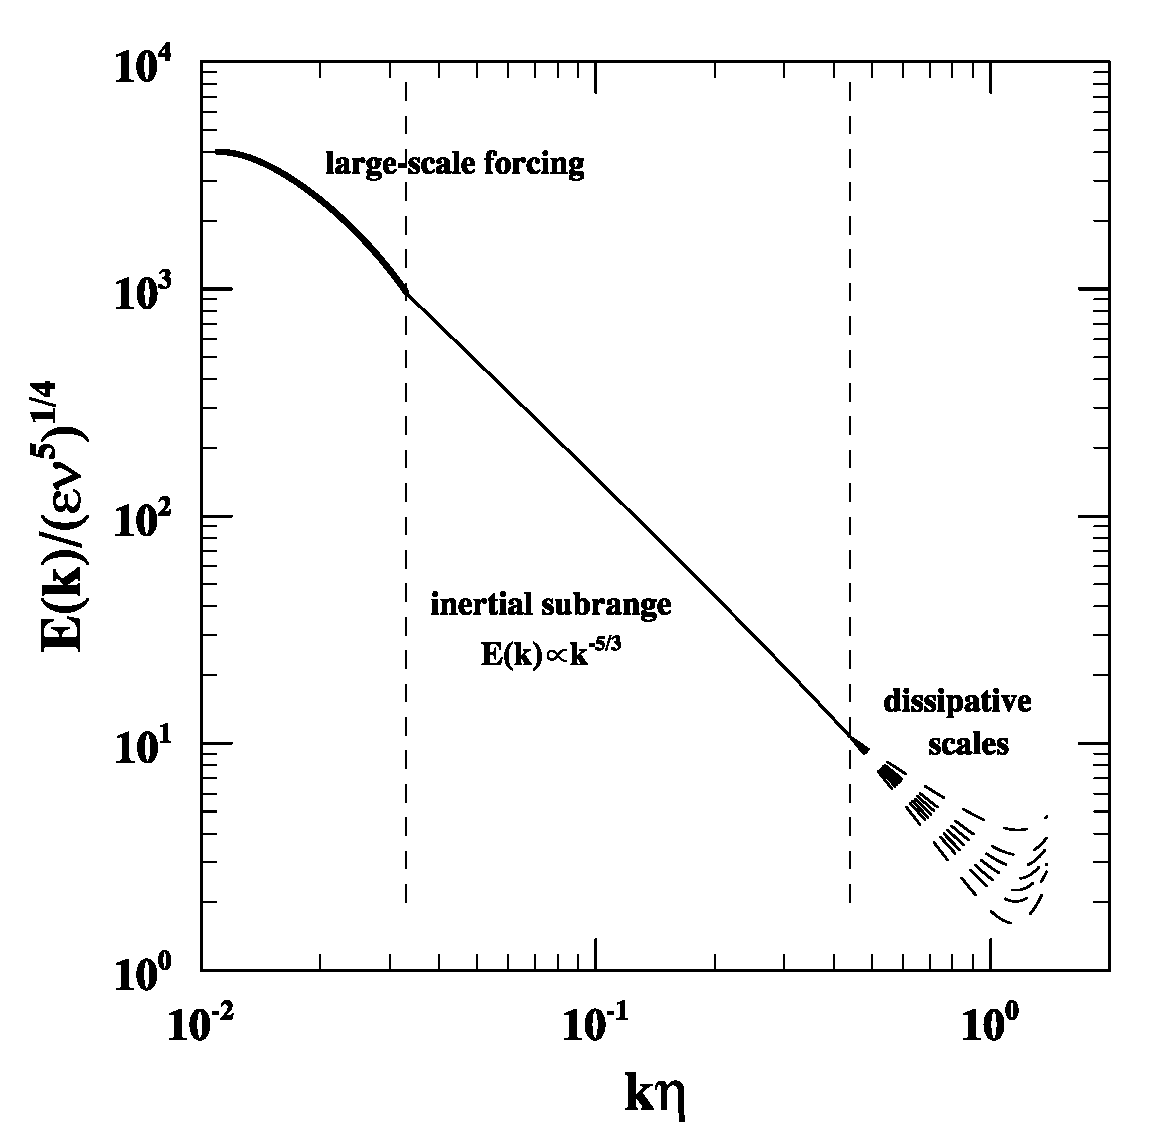
\includegraphics[width=10cm]{img/plots/1_1_forcing.pdf}
\caption{
The basic idea of deterministic forcing scheme: energy is supplied on large scales by fixing it for small wavenumbers (bold line), then it is transferred following Kolmogorov energy cascade ($E(k) \propto k^{-5/3}$) in inertial subrange, to finally reach smallest dissipative eddies represented by largest resolved wavenumbers (when $k_{\max} \eta \sim 1 = 10^0$, diverging dashed lines), that have largest influence on measured particle statistics at contact distances. Both axes are using standard normalisations (see Section \ref{ssc:ch2.flow.spec}) and logarithmic scale, that makes $k^{-5/3}$ curves appear as straight lines.}
\label{fig:forcing}
\end{figure}

The basic idea behind deterministic forcing scheme, as laid out in \textcite{Sullivan1994}, is to set energy associated with lowest wavenumbers in spectral space (or, equivalently, largest eddies) to predetermined values in every time step.
In order not to affect the entire flow, this is done for very few wavenumbers only ($|k| \in \{ 1, 2 \}$ in this study).
Then, due to energy cascade that characterises inertial scales of turbulence, the energy injected at low wavenumbers is transferred to the higher ones, allowing to achieve statistically stationary state with desired characteristics of homogeneous isotropic turbulence (see Figure \ref{fig:forcing}).
It~is accomplished by balancing large-scale energy input provided by the forcing term, and energy depletion due to viscous dissipation at small scales. 
In case of this study, the contribution from the deterministic forcing is included in Navier-Stokes equations in spectral space (i.e.~Fourier-transformed version of Equations \ref{eqn:n-s}, see Equation \ref{eqn:mom-spec} in Appendix A) as $\hat{\mathbf{f}}$.
Here, following the setup used in \textcite[p. 6]{Rosa2011}, the values for 3D shells associated with two lowest wavenumbers ($0.5 < |\textbf{k}| < 1.5$ and $1.5 < |\textbf{k}| < 2.5$) are set to $0.555440$ and $0.159843$ (following Kolmogorov's $E(k) \propto k^{-5/3}$ spectrum), respectively.
For remaining, larger wavenumbers, $\hat{\mathbf{f}}$ is zero, thus any smaller scales are not directly affected by forcing term.

\section{Large-Eddy Simulations}
\label{sc:ch1.les}

The pseudo-spectral method, as described above, is used in DNS to directly calculate the~velocity field of turbulent flow for all grid nodes.
Despite the important advantages, the~method faces huge challenges in implementation for massively parallel computers \parencite{Onishi2013}. 
Moreover, when applied to DNS, it features problematic limitations in computational performance and scalability. 
Therefore an alternative approach is proposed, so called large-eddy simulation (LES). 
The main goal is to reduce the size of computational grid without losing ability to model systems with similar range of turbulent scales, as measured by Taylor microscale Reynolds number, $R_{\lambda}$.
This is achieved by directly resolving turbulent flow only for~large and intermediate scales, while replacing direct resolution of small-scale turbulence (as~it~is~done in DNS) with one of the proposed models of turbulence, referred to as \emph{subgrid scale} (SGS) model.
Since we are replacing direct resolution with parameterisation, it is expected that the fidelity of results obtained using LES (when compared with DNS) may be~diminished, and they may be highly sensitive to the appropriate choice of the subgrid scale model.
On the other hand, this allows us to significantly reduce the size of used grid, and, consequently, increase computational performance of simulations, or enable simulations that achieve much higher $R_{\lambda}$.
This is possible because large part of computational effort in DNS is dedicated to resolving smallest turbulent scales \parencite[p. 558]{Pope2000}.
In case of this study, we use $N=64$ for LES and $N=256$ for DNS, thus the total number of grid nodes where fluid velocity field is directly resolved is reduced by the factor of $64$ (while still achieving comparable values of $R_{\lambda}$).
Conceptually, we may consider that each LES cell encompasses $4^3=64$ DNS cells where small-scale variations in velocity field would be directly resolved by~integrating Navier-Stokes equations (see Figure \ref{fig:dns-les-grids} for illustration).

\begin{figure}[h]
\centering
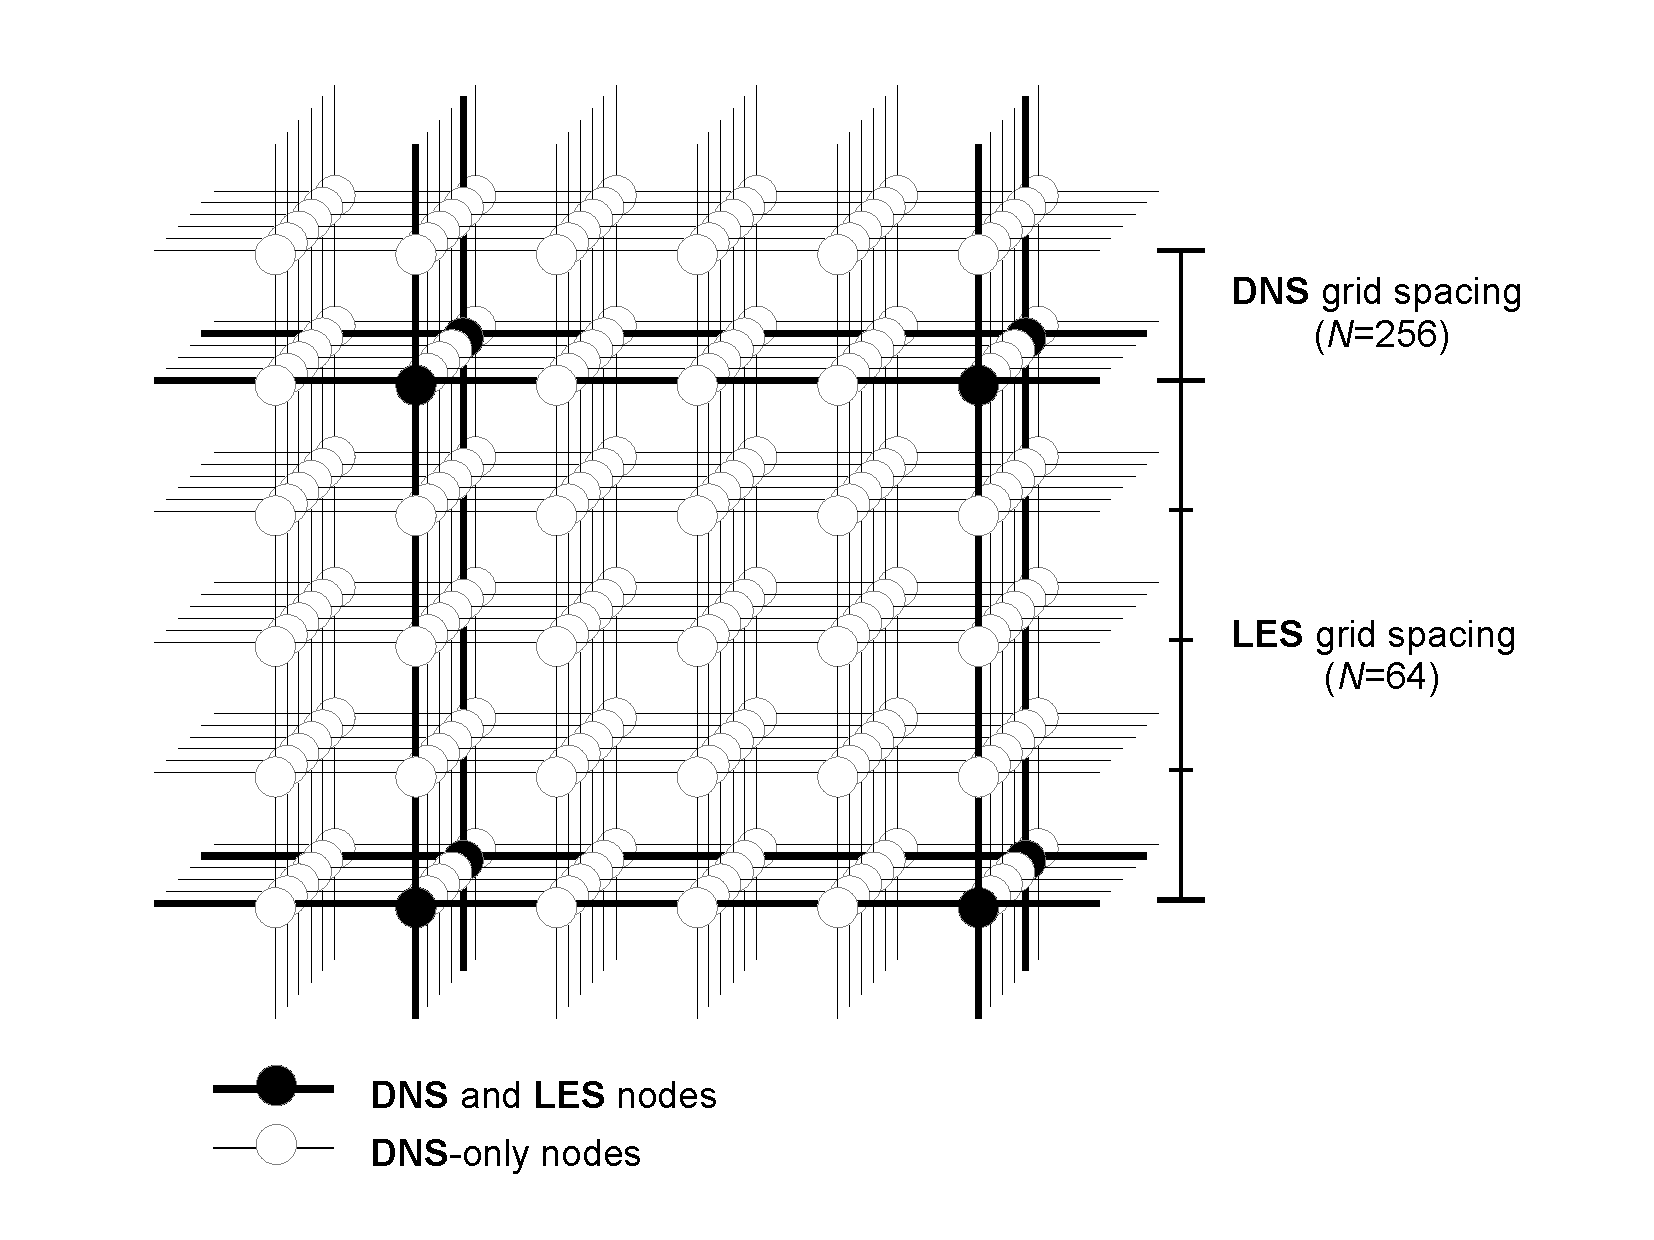
\includegraphics[width=17cm]{img/figs/dns-les-grids.pdf}
\caption{
Conceptual juxtaposition of computational grids for DNS and LES. In LES, the subgrid scale modelling parameterises small-scale turbulence that is directly resolved by $4 \times 4 \times 4$ block of cells in DNS.
}
\label{fig:dns-les-grids}
\end{figure}

In this study, that may be considered continuation of \textcite{Rosa2017}, very similar setup for LES method is employed \parencite[based on earlier work by ][]{Jin2010}.
In~particular, the closure of the subgrid term is based on the concept of the \emph{spectral eddy viscosity}, $\nu_{e}$.
In~spectral space, we consider filtered velocity field $\hat{\bar{\mathbf{U}}}(\mathbf{k}, t)$ that is governed by the following momentum equation \parencite{Pope2000}
\begin{equation}
\left\lbrace \frac{\partial}{\partial t} + [\nu + \nu_{e}(k|k_{c})]k^{2} \right\rbrace \hat{\bar{\mathbf{U}}}(\mathbf{k}, t) = \mathbf{P}(\mathbf{k}) \mathcal{F}(\bar{\mathbf{U}} \times \bar{\boldsymbol{\omega}}) + \hat{\mathbf{f}}(\mathbf{k}, t) ,
\label{eqn:les}
\end{equation}
where $\mathbf{P} \equiv \left\{ \mathbf{P}_{ij} \right\}$ is the projection tensor (see Equation \ref{eqn:proj-tensor}) and $\mathcal{F}$ -- Fourier transform.
By $k_{c}$ we denote cutoff wavenumber for filtering and its value is set using the same formula as maximal resolved wavenumber, $k_{\max}$, in DNS, i.e. $k_c = \left\lfloor \frac{N - 3}{2} \right\rfloor$ (for $N=64$, we have $k_c = 30$).
In this method of modelling turbulence sharp spectral filter is used to separate filtered (resolved) and residual (modelled) velocity fields which are strictly separated from each other in the spectral space with $| \mathbf{k} | = k_c$ as the boundary.
Hence, modelled modes for $| \mathbf{k} | > k_c$ have no bearing on turbulence model for larger wavenumbers and all necessary information on filtered velocity field $\mathbf{\hat{\bar{U}}}(\mathbf{k}, t)$ is contained in wavenumbers smaller than $k_c$.
Conversely, filtered velocity field contains no information on residual (small-scale) motions, thus they have to be entirely modelled \parencite[p. 615]{Pope2000}.

In equation \ref{eqn:les}, the term $\nu_{e}(k|k_{c})k^{2} \hat{\bar{\mathbf{U}}}(\mathbf{k}, t)$ represents specific the subgrid scale model used for parameterisation of small-scale turbulence.
Here, following \textcite{Rosa2017}, a~standard formula for the spectral eddy viscosity is used \parencite[see][]{Chollet1981}.
In~particular, the eddy viscosity is given by
\begin{equation}
\nu_{e}(k|k_{c}) = \nu_{e}^{+}(k|k_{c}) \sqrt{\frac{E(k_{c})}{k_c}} ,
\label{eqn:sgs-1}
\end{equation}
where total spectral energy for threshold wavenumber, $E(k_c)$, is dynamically evaluated at~each time step, while the remaining term depends on $k$ and is defined as follows
\begin{equation}
\nu_{e}^{+}(k|k_{c}) = C_{K}^{-3/2} [ 0.441 + 15.2 \exp( -3.03 k_{c} / k) ] ,
\label{eqn:sgs-2}
\end{equation}
where $C_{K}$ is the model constant (here, we set $C_{K} = 2.5$).

\medskip

LES is a well-established method in simulation of turbulent flows in many fields of research, and recently it is gaining more and more recognition as a tool for resolving carrier fluid flow in~particle-laden simulations.
The main issue with LES, i.e. unavailability of turbulent velocity field for small dissipative scales, may not be a huge concern for some experiments, mainly relating to some single-particle statistics, such as one-particle dispersion coefficient \parencite{Yang2008}.
Still, some single-particle statistics, such as average settling velocity, are affected by phenomena like preferential sweeping that depend on small-scale fluid motion, and thus are influenced by subgrid scale modelling \parencite{Rosa2017,Tom2019}.
Moreover, two-particle collision statistics are clearly influenced by small-scale velocity field, which is missing in LES \parencite{Jin2010}.
In most cases, studies show that elimination of directly resolved fine-scale turbulence may influence preferential concentration of inertial particles (in cases covered by this thesis it is usually reduced, but it may also be amplified, see \textcite{Fede2006} for more details).
Several studies established that such dependence on small turbulent scales is most prominent when Stokes number, $St$, of the system is close to $1$ \parencite{Wang2000,Pozorski2009,Jin2010}, and that is where most significant discrepancies between DNS and LES should manifest.
In contrast to the particle concentration (as measured by the radial distribution function), other collision statistics, such as the radial relative velocity (see Section \ref{ssc:ch2.coll.rdfrrv}) are to some extent governed by particle interactions with large-scale eddies \parencite{Wang2000}, and therefore their accuracy should be much less affected in LES. 
Determining the impact of LES parameterisation on such statistics is one of the main goals of this thesis.
This overview, however, shows that establishing relations between particle statistics, the ranges of turbulent scales that affect them, and possible impact of filtering out contribution of small eddies on particle behaviour is not a straightforward task.

\medskip

Note, that \textcite{Jin2010} and \textcite{Rosa2017} also consider intermediate method between DNS and LES, which is referred to as either \emph{filtered} DNS or LES \emph{a priori}.
It uses the same size grid as DNS and directly resolves turbulent flow for all scales, including the smallest.
Such velocity field, however, before it is used to calculate momentum transfer to particles (see Equation \ref{eqn:owc}), is filtered in spectral space by setting all values of $\hat{\mathbf{U}}(\mathbf{k}, t)$ to zero for large wavenumbers above filtering threshold (i.e. for $|\mathbf{k}| > k_c$).
Hence, particles are affected by filtered flow without directly resolved small-scale turbulence, as in LES.
On~the~other~hand, the flow itself is evolved with the same resolution as in DNS, providing more precise evolution of the fluid velocity field.
For the purpose of this study, filtered DNS is not of great interest, since it requires grids as large as for DNS, thus provide no viable improvement in method scalability and performance.
   

\section{Modelling Interactions between Fluid Flow and Particles}
\label{sc:ch1.part}

The population of particles contained within given system is modelled using Lagrangian approach, thus each (computational) particle is individually tracked.
Hence, given total number of particles, $N_{\text{part}}$, $k$-th particle, where $k \in \{ 1, \ldots , N_{\text{part}} \}$ is characterised by its position -- $\mathbf{Y}^{(k)}(t)$, velocity -- $\mathbf{V}^{(k)}(t)$, and other relevant properties, such as physical radius -- $a^{(k)}$.
In~case~of~this~study, not only radius of any single particle is constant throughout the entire simulation, but only \emph{monodisperse} systems are considered, i.e. systems where all particles have the same size (i.e. $a^{(k)} = a$ for all $k$).
Note, that since Lagrangian tracking is employed, particles may assume any positions within domain, not only at locations of grid points where values of fluid velocity field are directly available.
For that reason, proper interpolation techniques must be used when interactions between two phases are taken into account.

First, we consider advancement in time of velocity and position vectors of $k$-th particle affected by the carrier fluid with velocity field, $\mathbf{U}(\mathbf{x}, t)$.
For systems with large enough ratio between particle and fluid density, such as atmospheric clouds, we may apply simplified equations of motion \parencite{Maxey1983}.
For $k$-th particle we have
\begin{equation}
  \left\{
  \begin{array}{ll}
  \frac{d \mathbf{V}^{(k)}(t)}{d t} = - f (Re_p) \frac{ \mathbf{V}^{(k)}(t) - \mathbf{U}(\mathbf{Y}^{(k)}(t), t) }{\tau_{p}} + \mathbf{g} ,\\
  \frac{d \mathbf{Y}^{(k)}(t)}{d t} = \mathbf{V}^{(k)}(t) ,
  \end{array}
  \right.
  \label{eqn:owc}
\end{equation}
where $f$ is the drag correction factor (in this study $f = 1$), $Re_p = (2 a \rho V_{\text{rel}}) / \mu $ -- particle Reynolds number, $V_{\text{rel}}$ -- particle-fluid relative velocity, $\tau_{p} = (2 \rho_{p} a^{2}) / (9 \mu)$ -- Stokes inertial response time of a particle, $\rho_{p}$ -- particle density, $\mu$ -- dynamic viscosity of the fluid, and $\rho$ -- density of the fluid.
These equations, as stated before, hold when $\rho_p \gg \rho$ (in case of water droplets in air, $\rho_p / \rho \approx 10^3$). 
The gravitational acceleration is given as $\mathbf{g}$, which may be either zero (for simulations without gravity), or set to $980.67 \, \text{cm} / \text{s}^{2}$ and pointing vertically downwards. 
Furthermore, expression $\mathbf{U}(\mathbf{Y}^{(k)}(t), t)$ denotes contribution from the velocity field of the carrier fluid in the current location of $k$-th particle, and it is calculated using six-point Lagrangian interpolation in each spatial direction \parencite{Ayala2014}.
Effects due to the finite size of actual, spherical particles (as opposed to point-particle representation) may be neglected, since considered radii of water droplets ($20$~$\upmu\text{m}$ -- $60$~$\upmu\text{m}$) are significantly smaller than the Kolmogorov length scale of the turbulence, $\eta$. 
Equations \ref{eqn:owc} are integrated using fourth-order Adams-Moulton and fourth-order Adams-Bashforth methods, respectively.

The procedure described above incorporates calculation of the particle motion, as~well~as the influence of the carrier fluid on particles due to momentum transfer.
When simulations are limited to above description of fluid-particle interactions, they are said to involve \emph{one-way momentum coupling} (OWC).
These simulations require less computational resources and have been shown to effectively model dilute systems.
In general, we use particle mass loading, $\Phi_{m}$, as the global measure of relative amount particles in the system.
It is defined as the ratio of~total mass of particles to total mass of carrier fluid contained in the system, i.e.:
\begin{equation}
\Phi_m = \Phi_V \frac{\rho_p}{\rho} = \frac{(4/3) \pi a^3 N_{\text{part}}}{L^3} \frac{\rho_p}{\rho} ,
\label{eqn:phim}
\end{equation}
where $L$ denotes the side-length of simulation domain.
Here, $\Phi_V$ denotes particle volume fraction, which is used as an alternative measure of amount of particles in the system.
When particle content becomes larger (approximately, for $\Phi_m > 0.1$), OWC approach becomes insufficient, and other interactions should be considered as well.
Promising strategy, not discussed further in this study, is to account for interactions between particles through disturbance field that models aerodynamic interactions between particles, as in Hybrid DNS method \parencite[see e.g.][]{Ayala2014}.
Another remedy is to account for the transfer of momentum in the other way as well, i.e. from particles to the carrier fluid.
Such approach not only allows to~study influence of particles on the fluid flow characteristics and turbulence modulation, but also, indirectly, provides a limited way to include interactions between particles as mediated by~the~fluid flow that is disturbed by the presence of nearby, slowly approaching particles.
These simulations are said to involve \emph{two-way momentum coupling} (TWC).

In TWC approach, we assume that cumulative force per unit mass exerted by particles on~the~fluid, denoted by $\mathbf{f}^{(p)}$ in Equation \ref{eqn:n-s}, is non-zero.
Such contribution may be expressed as follows \parencite{Bosse2006,Monchaux2017,Rosa2022}:
\begin{equation}
\mathbf{f}^{(p)}(\mathbf{x}, t) = - \frac{M}{\rho_{p}} \sum_{k=1}^{N_{\text{part}}} m^{(k)}_{p} \left( \frac{ \mathbf{U}(\mathbf{Y}^{(k)}(t), t) - \mathbf{V}^{(k)}(t) }{\tau_{p}} \right) \delta \left( \mathbf{x} - \mathbf{Y}^{(k)}(t) \right) ,
\label{eqn:twc-th}
\end{equation}
where most of the notation follows that from Equation \ref{eqn:owc}, except $m^{(k)}_{p}$ which denotes individual mass of $k$-th particle.
Moreover, $M$ is the weighting (super-particle) factor, discussed later in this section.
This continuous description involves summation of contributions from all particles (terms that, according to Newton's third law, are equal in magnitude and opposite in direction to terms in Equation \ref{eqn:owc}), and localised in given spatial point $\mathbf{x}$ with Dirac delta distribution.
In practice, we need a convenient way to calculate $\mathbf{f}^{(p)}$ for positions $\mathbf{x}$ at grid points without need to iterate over all particles.
Due to mismatch between actual particle positions and discrete locations of grid points we use mollified Dirac delta, so that strict particle locality is relaxed and their contributions may be projected onto adjacent grid nodes.
Thus,~Equation \ref{eqn:twc-th} becomes
\begin{equation}
\mathbf{f}^{(p)}(\mathbf{x}, t) = - \phi_{m}(\mathbf{x}, t) \left( \frac{ \mathbf{U}(\mathbf{x}, t) - \mathbf{V}_{E}(\mathbf{x}, t)}{\tau_{p}} \right) ,
\label{eqn:twc-px}
\end{equation}  
where $\phi_{m}$ is local mass loading. 
The term $\mathbf{V}_{E}(\mathbf{x}, t)$, is referred to as Eulerian particle velocity at location $\mathbf{x}$, and may be computed as follows:
\begin{equation}
\mathbf{V}_{E}(\mathbf{x}, t) = \sum_{k=1}^{N_{\text{part}}} \mathbf{V}^{(k)}(t) \, \sigma(|| \mathbf{x} - \mathbf{Y}^{(k)}(t) ||) ,
\label{eqn:twc-ve}
\end{equation}
where $\sigma$ is the interpolation kernel used to determine effect of given particle, based on its location, $\mathbf{Y}^{(k)}(t)$, onto grid node located at $\mathbf{x}$.
There are several choices of such kernels and their practical implementations \parencite{Garg2007}, but in this study the \emph{projection onto neighbouring nodes} (PNN) is used exclusively.
Instead of summing all particle forces around a node, particle force contribution is projected onto $8$ neighbouring nodes based on some weighing scheme.
Such scheme, in general, is a standard bi- or tri-linear function, that depends on separation distance between particle and grid node.
Here, in particular, we~use calculations based on cell volume partition (see Figure \ref{fig:pnn}) introduced in \textcite{Squires1990}.
This interpolation procedure is justified when influence of particles on the fluid is~indeed highly localised and limited to the closest neighbouring nodes.
In practice, this takes form of requirements that size (radius, $a$) of a particle must be smaller than both spatial grid spacing, $\Delta x$, and smallest resolved turbulent scales, as measured by Kolmogorov length scale, $\eta$.
Both conditions are satisfied for all simulations in this study (see Section \ref{ssc:ch2.flow.part}).

Note, as well, that in systems with TWC, a mean flow must appear due to the net influence of all particles on the fluid (especially if gravity is concerned), which violates periodicity condition and leads to instability of computations.
For that reason, at every time step, the~Fourier mode corresponding to mean flow (i.e. for $|\mathbf{k}| = 0$) is zeroed, which is equivalent to applying a pressure gradient countering the mean flow, which does not affect validity of~the~statistical results.
Another numerical artefact of TWC may be the indirect effect of~$\textbf{f}^{(p)}$ on the continuity equation, causing the resulting velocity field to be not divergence-free.
This issue was addressed in \textcite{Rosa2020}, as this effect is not significant in simulations performed here, since the volume fraction of particles compared to fluid is relatively small (at~most of~order~$10^{-3}$).
Moreover, pseudo-spectral method computations enforce constraint from continuity equation by projecting the velocity vector onto plane normal to 3D wavenumber $\mathbf{k}$ (which also eliminates direct dependence on pressure, see Appendix \ref{app:psm} for more details).

\begin{figure}[h]
\centering
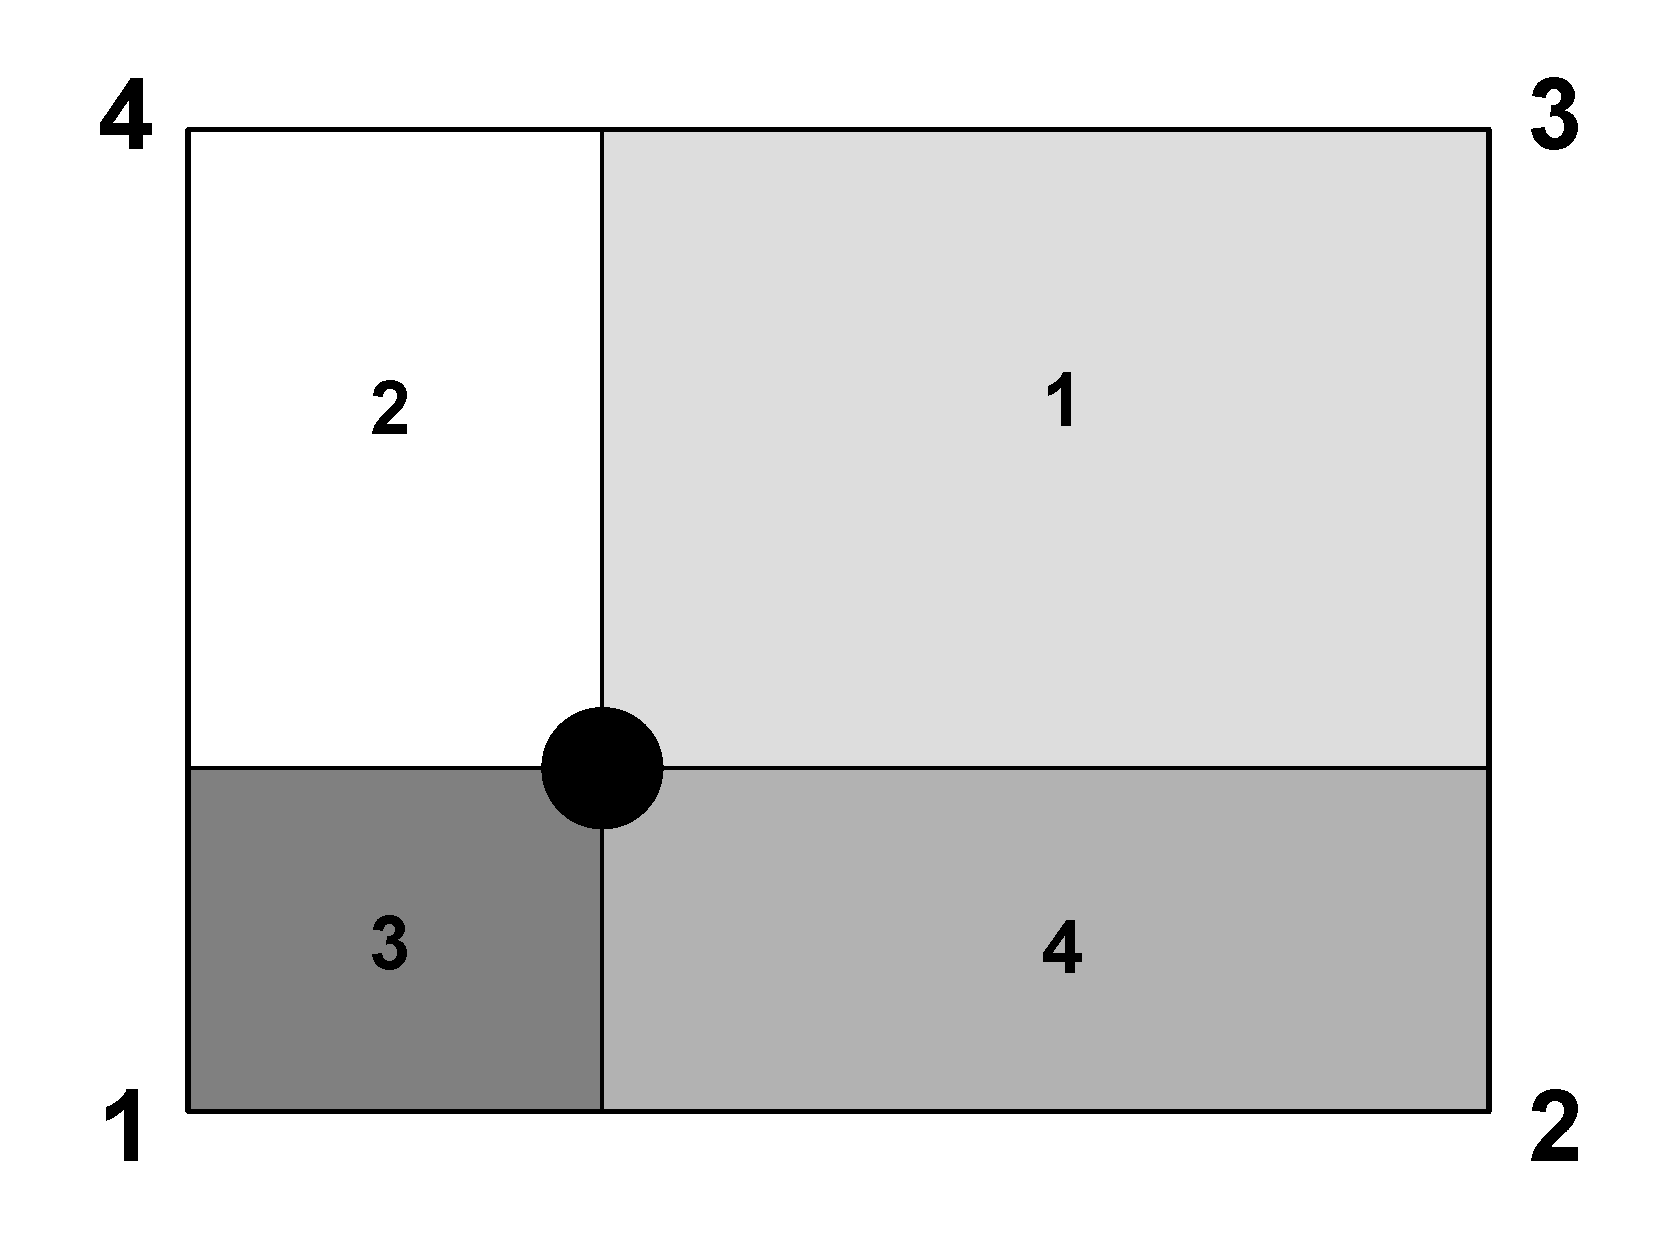
\includegraphics[width=8cm]{img/figs/pnn.pdf}
\caption{
Projection onto neighbouring nodes (PNN; simplified illustration for 2D case) -- contribution of the particle momentum to the fluid momentum at a grid node depends on the separation distance. For example, the particle force may be projected onto neighbouring nodes using weights which are proportional to cell areas or volumes in 3D. Here, the fluid flow at grid node 1 is affected by a fraction of the particle Stokes drag proportional to the area with marker 1, and so on. Based on~\textcite[Fig. 1]{Garg2007}.}
\label{fig:pnn}
\end{figure}

\medskip

The total number of particles, $N_{\text{part}}$, is another parameter, besides grid size $N$, that~mainly determines computational burden of simulations.
In this study, highest number of individually tracked particles was 20 million, and for droplets with smaller radii (and, consequently, mass) that was still not sufficient to achieve higher values of the mass loading.
Still, simulations with larger mass loading ($0.1 < \Phi_{m} < 1$) are necessary to clearly observe effects of~two-way momentum coupling on measured statistics.
For that reason, in some simulations, \emph{super-particle parameterisation} was used to increase $\Phi_m$ without adding new computational particles \parencite{Elghobashi1994}.
That parameterisation is applied by using \emph{weighting factor} $M$ in~Equation \ref{eqn:twc-th}.
For $M=1$, each computational particle represents exactly one droplet, hence no extra parameterisation is present.
For $M > 1$, however, every computational particle models a cluster of $M$ droplets (so-called \emph{super-particle}) that is tracked together as~a~single computational point-particle with inflated mass by the factor of $M$.

Such parameterisation was used in \textcite{Rosa2020} for similar reasons, and it was observed that it does not significantly affect measured collision statistics, as long as $M$ is not too large.
Moreover, it was observed that these discrepancies are relatively small when mass loading is large, probably this is due to stronger turbulence attenuation in simulations without gravity (turbulence is the main mechanism enforcing particle clustering).
On the other hand, in simulations with gravity, a larger mass loading results in the formation of new vortical structures, which cause the decorrelation of particle motion and consequently a more uniform spatial distribution.
More systematic analysis of the impact of this parameterisation was conducted in recent study by \textcite{Rosa2022}, where collision statistics from simulations with varying $M$ and fixed mass loading, $\Phi_m$, were analysed.
The clear tendency for that parameterisation to overestimate the radial relative velocity and underestimate the radial distribution function was reported.
For values of $M < 20$ the influence of the super-particle parameterisation may be acceptable, but otherwise discrepancies rapidly cumulate and render obtained results applicable for only qualitative analysis at best (in some cases, for $M = 100$, values of RDF were halved, and for RRV inflated by the factor of $3$).
Also, larger discrepancies were observed in simulations with gravity. 

Interestingly, some studies using more refined techniques of dealing with super-particles \parencite{Garg2009} have shown that errors arising from that parameterisation increase with~refinement of the grid.
This may be beneficial when considering LES method, as it works on~much~coarser grid than comparable DNS.
Still, cumulative effects and possible interactions between these two parameterisations may be quite complex and hard to follow in a systematic and quantitative manner.



\section{Notes on Implementation}
\label{sc:ch1.impl}

The effective implementation of the methods presented above is necessarily intended for massively parallel computation environments (supercomputers) due to large grids and particle populations required to produce physically meaningful results.
The solver code used in this study was long developed, tested, and improved upon to provide further capabilities \parencite[see~e.g.][]{Ayala2014,Parishani2015}, including modifications necessary to obtain results presented here.
It is implemented using Message Passing Interface (MPI) to facilitate communication between several processes executing the code.
The division of work is based on~the~concept of 2D domain decomposition, where each process is handling all computations associated with one part (subdomain) of the entire computational domain.
In this case, the~domain is divided along two out of three spatial axes into ''columns'' with equal number of~grid nodes (see Figure \ref{fig:2dd}).
By default, the two directions chosen for decomposition are~those orthogonal to the (vertical) direction of gravity, in order to minimise the number of~particles crossing the subdomain boundaries. 
This strategy is relatively simple to implement and quite efficient, if we assume that distribution of particles between subdomains is close to uniform (this assumption will be further analysed in Section \ref{sc:ch3.perfp}).
In this study, subdomains have dimensions $16 \times 16 \times N$ to provide large enough margin for convenient communication between processes.
In particular, for DNS and its grid with $256^{3}$ nodes we have $16^{2} = 256$ subdomains, and for LES, with $64^{3}$ grid -- $4^{2} = 16$ subdomains.
The number of processes used to execute solver code is equal to the number of subdomains used.

\begin{figure}[h]
\centering
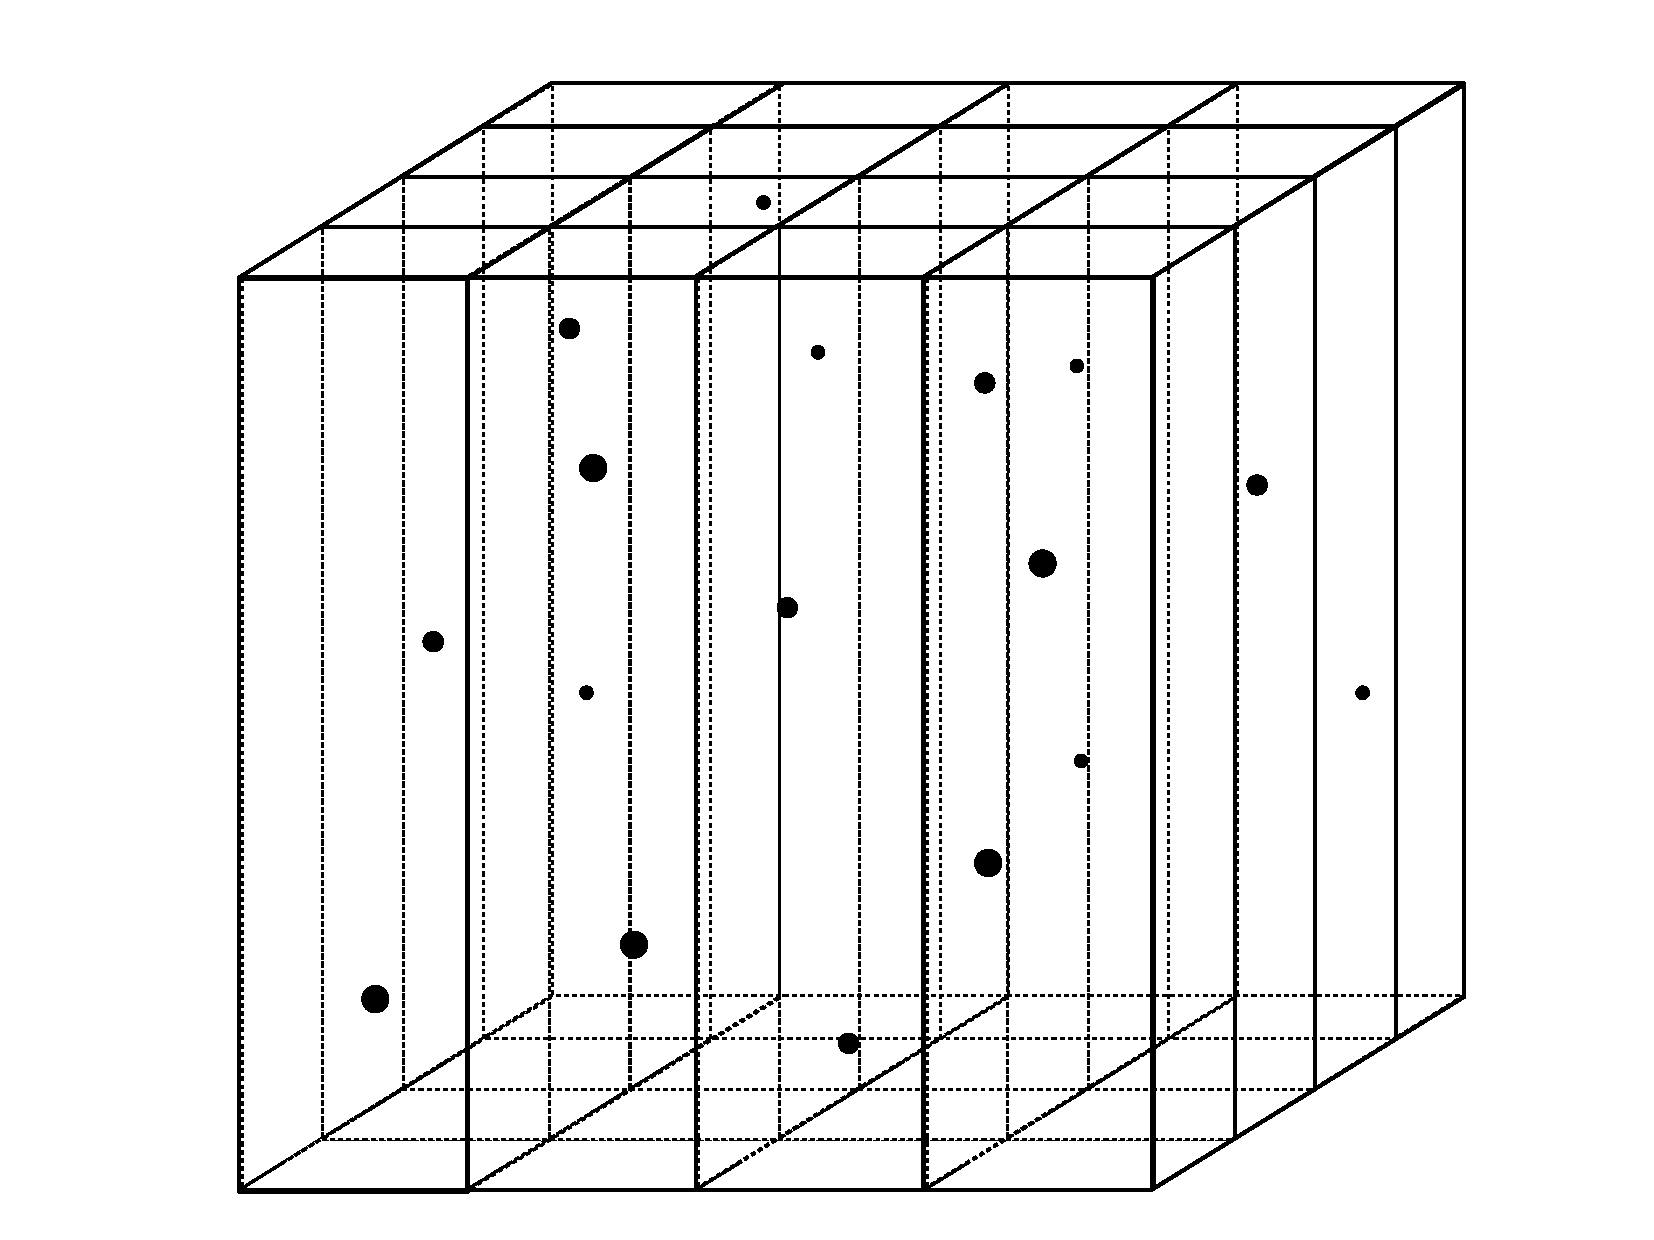
\includegraphics[width=10cm]{img/figs/2dd.pdf}
\caption{
Schematic representation of 2D domain decomposition. This image corresponds to actual decomposition of $64^{3}$ grid used for LES. Entire domain is divided into $4 \times 4 = 16$ subdomains, each~with~$16 \times 16 \times 64$ nodes.
}
\label{fig:2dd}
\end{figure}

Exact steps that constitute each iteration of both DNS and LES method are summarised in Table \ref{tab:code-steps}.
In general, entire code may be divided into parts that handle computations involving either fluid flow or particle motion, as well as parts used for data post-processing (i.e. to calculate and output interesting statistics of fluid flow and particles, not necessarily executed in every iteration).
The heart of pseudo-spectral code is the efficient implementation of the fast Fourier transform, as every iteration requires performing 3D FFT three times.
Parallel implementation of 3D FFT is used as proposed by \textcite{Ayala2013}, where it~is~decomposed into three separate calls to 1D FFT procedures provided by \texttt{fftw} library along with an original procedure for data transposition.
The choice of 2D domain decomposition was mainly driven by the fact that it was found to be optimal for such implementation of parallel 3D FFT.  
It was chosen above 1D decomposition that was initially proposed by \textcite{Dmitruk2001}, since it heavily restricted number of parallel processes allowed to execute the code, and above 3D decomposition, which introduced excessive costs of communication and data transfer between larger number of subdomains \parencite{Ayala2013}.   
The architecture used to store particle data and transfer it between processes is a key part of the implementation, as~detection of nearby particles is crucial for efficient calculation of two-point particle collision statistics.
For that reason the concept of linked lists together with the cell-index method was employed according to \textcite[p. 149--152]{Allen1987}.
In every run, statistics of~the~fluid flow and particles statistics are gathered only after the entire system has reached~the~statistically stationary state, which is not earlier than after approximately $10 T_e$ \parencite{Rosa2017}, where $T_e$ is turnover time for largest resolved eddies.  


\chapter{Physical Fidelity of DNS and LES Results}
\label{ch:ch2}

This Chapter focuses on ascertaining the physical fidelity of LES results in comparison with those provided by DNS.
Since LES partially replaces direct resolution of flow with subgrid scale parameterisation, some difference of results is expected.
This is also true for particle statistics at contact distance are concerned, as they are sensitive to the effects of turbulence, especially at smaller length scales.
In this chapter, basic statistics and energy spectra of background turbulent flow shall be presented for both methods, followed by statistics related to particles and the effects of turbulence modulation by particles in TWC simulations.
More importantly, broader analysis of key particle collision statistics -- radial distribution function, radial relative velocity, and collision kernels -- is provided, with results from both DNS and LES.
Simulations with both one- and two-way momentum coupling are considered, both with and without gravity.



\section{Turbulent Flow Statistics}
\label{sc:ch2.flow}

The standard procedure in simulations using the pseudo-spectral code introduced in Chapter \ref{ch:ch1} is to obtain statistically stationary fluid flow without introducing any particles into the~system and estimate its statistics as a reference.
These statistics shall be discussed in two following sections.
Later, such background flow is randomly seeded with particles, and entire system is simulated until stationary state is restored, and particle statistics may be collected, as detailed in Section \ref{ssc:ch2.flow.part}.
Such approach not only reduces time required by particle-laden simulations to achieve desired state, but also  -- in case of two-way coupling -- provides baseline for studying influence of particles on the statistics of underlying turbulence.



\subsection{Basic Statistics of Turbulent Flow}
\label{ssc:ch2.flow.bstat}

When no specific boundaries are defined, the model of homogeneous and isotropic turbulence is abstracted from any physical scale. 
More precisely, without introduction of reference objects with well defined physical dimensions (e.g. domain boundaries, or -- as in this study -- particles with well defined physical radii) the parameters of turbulence may be applied at arbitrary scales, from small cells of clouds to the global atmospheric circulation.
For that reason, parameters and statistics of turbulent flow presented below are expressed in nondimensional spectral (DNS) units, as the most important indicator is the range of turbulent scales being resolved and not physical size of the domain.
It should be added that the characteristic length scale results from the domain size. 
In turn, the time and velocity scales are determined by~the~rate~at~which the kinetic energy is supplied by the forcing scheme.

There are three main numeric parameters that influence the resulting turbulent flow and~its~statistics, which are -- for the most part -- fixed throughout all simulations in this study.
These include:
\begin{itemize}
\item the \emph{number of spatial grid nodes in each dimension}, $N$, which primarily determines range of turbulent scales that can be directly resolved in simulations (here $N=256$ for~DNS and $N=64$ for LES);
\item the \emph{numerical} (\emph{molecular}) \emph{kinematic viscosity of the fluid}, $\nu$, is an important parameter that is required to balance out the large-scale forcing with enough energy dissipation to obtain viable energy spectrum, and desired range of resolved scales of turbulence; in all simulations value of $1.5 \times 10^{-3}$ is used, as it ensures numerical stability and maximises obtained Reynolds number.
\item the \emph{time step}, $\Delta t$, is another parameter that ensures numerical stability of the simulation.
\end{itemize}
Note that for the particle-free flow time step must be set to a value that guarantees that Courant number is lower than $0.3$, which is established as a stability and accuracy threshold for pseudo-spectral method.
Recall, that \emph{Courant} (or \emph{Courant}--\emph{Friedrichs}--\emph{Lewy}, \emph{CFL}) \emph{number} is defined as follows:
$$ \text{CFL} = \max ( || \mathbf{U} ||_1 ) \frac{\Delta t}{\Delta x} , $$
where $|| \cdot ||_1$ is a 1-norm, maximum of which is taken over all nodes in the grid, and $\Delta x$ is spatial spacing, here equal to $(2 \pi) / N$. 
The default times step for most simulations was set to $9 \times 10^{4}$, but in some cases, due to complex interactions with particles, some adjustments were necessary (for more details, see discussion in Section \ref{ssc:ch2.flow.part}).

Beyond purely quantitative parameters, there are some more ''structural'' choices that implicitly affect simulations and their results.
One such important choice involves type of~forcing scheme being used (here we exclusively use deterministic scheme, see Section \ref{sc:ch1.pspec}).
Even more options come with LES method, where the choice of subgrid-scale model being used is crucial for the final outcome of simulations.
As discussed in Section \ref{sc:ch1.les}, this study employs spectral-eddy viscosity model that was already used in several previous studies \parencite{Yang2008, Jin2010, Rosa2017}.
Such model allows for some degree of~customisation, via model parameter $C_K$ (see Equation \ref{eqn:sgs-2}), which in this study was fixed at $2.5$.
Note, that all aforementioned studies used only stochastic forcing, and this one is the first -- according to author's knowledge -- where LES is used with deterministic forcing scheme (with pseudo-spectral solver).
For that reason, extra effort was made to validate proper choice of~$C_K$ parameter, as elaborated in Appendix \ref{app:sgs}. 

To gain some insight into properties of turbulence, we gather some standard flow statistics that are time- and volume-averaged over some period, in which statistically stationary state of the flow was attained.
Firstly, two basic statistics that are calculated directly from velocity field and energy spectrum of the flow are: 
\begin{itemize}
\item $u'$ -- \emph{root-mean-square (rms) of fluctuating velocity} -- standard deviation of the fluid velocity field with respect to the mean flow (which is ensured to be zero); physically, it~is~related to the intensity of turbulence; and
\item $\epsilon$ -- \emph{energy dissipation rate} -- rate at which turbulence kinetic energy is converted into thermal internal energy; it may be computed as follows:
\begin{equation}
\epsilon  = 2 \int_{k_{0}}^{k_{\max}} \nu k^{2} E(k) dk
\label{eqn:eps}
\end{equation}
where $E(k)$ denotes the turbulent kinetic energy associated with the wavenumber $k$ in spectral space, and $\nu$ is numerical kinematic viscosity.  
\end{itemize}
Furthermore, we provide some derived statistics that are commonly used to characterise different scales of turbulence. These include: $\eta$ -- the \emph{Kolmogorov length scale}, $\tau_{k}$ -- the \emph{Kolmogorov time scale}, $L_{s}$ -- the \emph{integral length scale}, $\lambda$ -- the \emph{transverse Taylor microscale}, $T_{e}$ -- the \emph{large-eddy turnover time}.
Finally, two important control and target statistics (besides CFL) are computed. These include:
\begin{itemize}
\item $R_{\lambda} = \frac{u' \lambda}{\nu}$ -- \emph{Taylor-microscale Reynolds number} -- Reynolds number associated with inertial subrange, used to measure the range of resolved turbulent scales (in this study, this value is meant to be maximised given fixed grid scale $N$); and
\item $k_{\max} \eta$ -- spatial resolution parameter that serves as an important control value in DNS; it should be minimised in order to maximise amount of resolved turbulence (i.e. $R_{\lambda}$), but its value must be greater than $1$ to ensure that fine scales of turbulence can be resolved.
\end{itemize}
Note, that for studies oriented towards maximising $R_{\lambda}$ (as this one is), it is customary to~aim for $1 < k_{\max} \eta < 2$, but in other studies resolution requirements may differ \parencite{Buaria2019}, as higher values of $k_{\max} \eta$ coincide with more numerical stability of simulations.
Also, in TWC simulations, it is argued that larger values of $k_{\max} \eta$ may be associated with more stability in inter-phase interpolation \parencite[see][]{Rosa2020}.   

Table \ref{tab:flow-stats} contains used parameters and gathered statistics of background turbulent flows for both DNS and LES.
The measurement uncertainties for these statistics were calculated as~in~\textcite{Rosa2013}, accounting for the autocorrelation of flow statistics in the statistically stationary state.
The parameters introduced above are calculated in a way specific for DNS simulations, and these may not directly translate to LES, however may serve as helpful indicators when comparing two methods (especially, $R_{\lambda}$).
There is no agreement between authors whether to present more \parencite{Rosa2017} or less \parencite{Yang2008} of such DNS statistics for LES as well.
This is mainly due to dependence of many statistics on numerical viscosity, $\nu$, which is modelled in subgrid-scale model, thus being dependent on wavenumber, $k$ (see Equation \ref{eqn:sgs-1}), and not constant as in DNS.
For that reason, most of statistics for LES in Table \ref{tab:flow-stats} (marked with asterisk) are listed with ''effective'' values, that are calculated in~a~way~that~includes influence of SGS modelling on viscosity (see Appendix \ref{app:sgs} for details). 

\begin{table}[h]
\centering
\begin{tabular}{llll}
 & & & \scriptsize{\textcite{Rosa2013}}  \\
 & \textbf{DNS} & \textbf{LES*} & \textbf{DNS}  \\ \hline
$N$ & $256$ & $64$ & $256$ \\
$\Delta t \cdot 10^{4}$ & $9.0$ & $9.0$ & $9.0$  \\
$\nu \cdot 10^{3}$ & $1.5$ & $1.5$ & $1.1$  \\

$u'$ & $0.871 \pm 0.001 $ & $0.861 \pm 0.001 $ & $0.868 \pm 0.002 $ \\
$\epsilon$ & $0.212 \pm 0.002 $ & $0.200 \pm 0.001$* & $0.200 \pm 0.003 $  \\

$\eta \cdot 10^{2}$ & $1.125 \pm 0.003$ & $2.078 \pm 0.007$* & $0.903 \pm 0.037$  \\
$\tau_{k} \cdot 10^{2}$ & $8.436 \pm 0.043$ & $15.755 \pm 0.122$* & $7.420 \pm 0.620$  \\
$L_{s}$ & $1.462 \pm 0.003$ & $1.501 \pm 0.004$ & $1.496 \pm 0.005$  \\
$\lambda \cdot 10$ & $2.851 \pm 0.011$ & $5.252 \pm 0.014$* & $2.494 \pm 0.015$  \\
$T_{e}$ & $3.616 \pm 0.028$ & $3.697 \pm 0.025$* & $3.774 \pm 0.045$  \\

$k_{\max} \eta$ & $1.423 \pm 0.004 $ & --- & $1.143 \pm 0.005 $  \\
$R_{\lambda}$ & $165.91 \pm 0.51 $ & $165.01 \pm 0.11$* & $196.87 \pm 0.78 $            
\end{tabular}
\caption{Parameters and statistics of background turbulent flows in spectral units simulated in this study (first two columns) and these by \textcite{Rosa2013}, shown for result validation (third column). All listed simulations used deterministic forcing scheme. (* -- in LES, statistics marked with * are ''effective'', i.e. calculated using viscosity adjusted by subgrid-scale model; for more details see Appendix \ref{app:sgs}.}
\label{tab:flow-stats}
\end{table}

First two columns refer to particle-free flows used for all simulations in this study, DNS and LES, respectively.
The remaining column is provided as a reference and for result validation.
DNS turbulent flow was simulated with similar parameters to the one used for numerical experiments with one-way momentum coupling in \textcite[Table 1, entry for $256^3$]{Rosa2013}, which are presented in third column of Table \ref{tab:flow-stats}.
Note, that slightly smaller value of viscosity used in that study resulted in smaller resolution parameter, and, consequently, $\sim 15\%$ larger Reynolds number.
Particularly interesting is the comparison between statistics for DNS and ''effective'' statistics for LES.
For statistics that are directly derived from either fluid velocity field ($u'$) or its energy spectrum ($\epsilon$), there is strong agreement.
The same is true for large scale parameters, $L_s$ and $T_e$.
What is most important, despite much smaller grid size, the~$R_{\lambda}$ in~both~cases is almost the same, due to the effects of the spectral eddy viscosity of subgrid-scale model.
Also $u'$, directly computed from fluid velocity field (independet from $\nu$), and associated with the magnitude of turbulence, assumes very close values for both DNS and LES.  
On the other hand, we can see increase (approximately by the factor of 2) in spatial and temporal scales (both small, $\eta$ and $\tau_k$) and intermediate ($\lambda$).
No statistics for LES are presented for comparison, such as, e.g. \textcite[Table 1]{Rosa2017}, since all other studies used stochastic forcing scheme, which makes obtained statistics not directly comparable.

\subsection{Energy and Dissipation Spectra}
\label{ssc:ch2.flow.spec}

The important insight and validation for any simulation of turbulent flow is the analysis of its energy and dissipation spectra.
Since the pseudo-spectral method naturally operates in Fourier space, the energy spectrum, $E(k)$, can be easily retrieved.
Such spectrum, for intermediate wavenumbers, may be compared with theoretical $(-5/3)$ Kolmogorov spectrum.
More specifically, for inertial subrange, we expect obtained spectra to closely coincide with:
\begin{equation}
E_{\text{Kolm}}(k) = C \epsilon^{2/3} k^{-5/3} ,
\label{eqn:kolm}
\end{equation}
where constant $C$ was experimentally determined to be $1.5$. 
Furthermore, the energy dissipation spectrum, $D(k)$, may be easily derived for $k \in \{ k_{0}, \ldots, k_{\max} \}$ using the following formula:
$$ D(k) = 2 \nu k^{2} E(k) . $$
Energy and dissipation spectra of turbulent flows obtained by DNS and LES are shown in Figures \ref{fig:spec} and \ref{fig:diss}, respectively.
For convenience, both spectra are shown in log-log plot with proper normalisation to ensure values are dimensionless.

\begin{figure}[h]
\centering
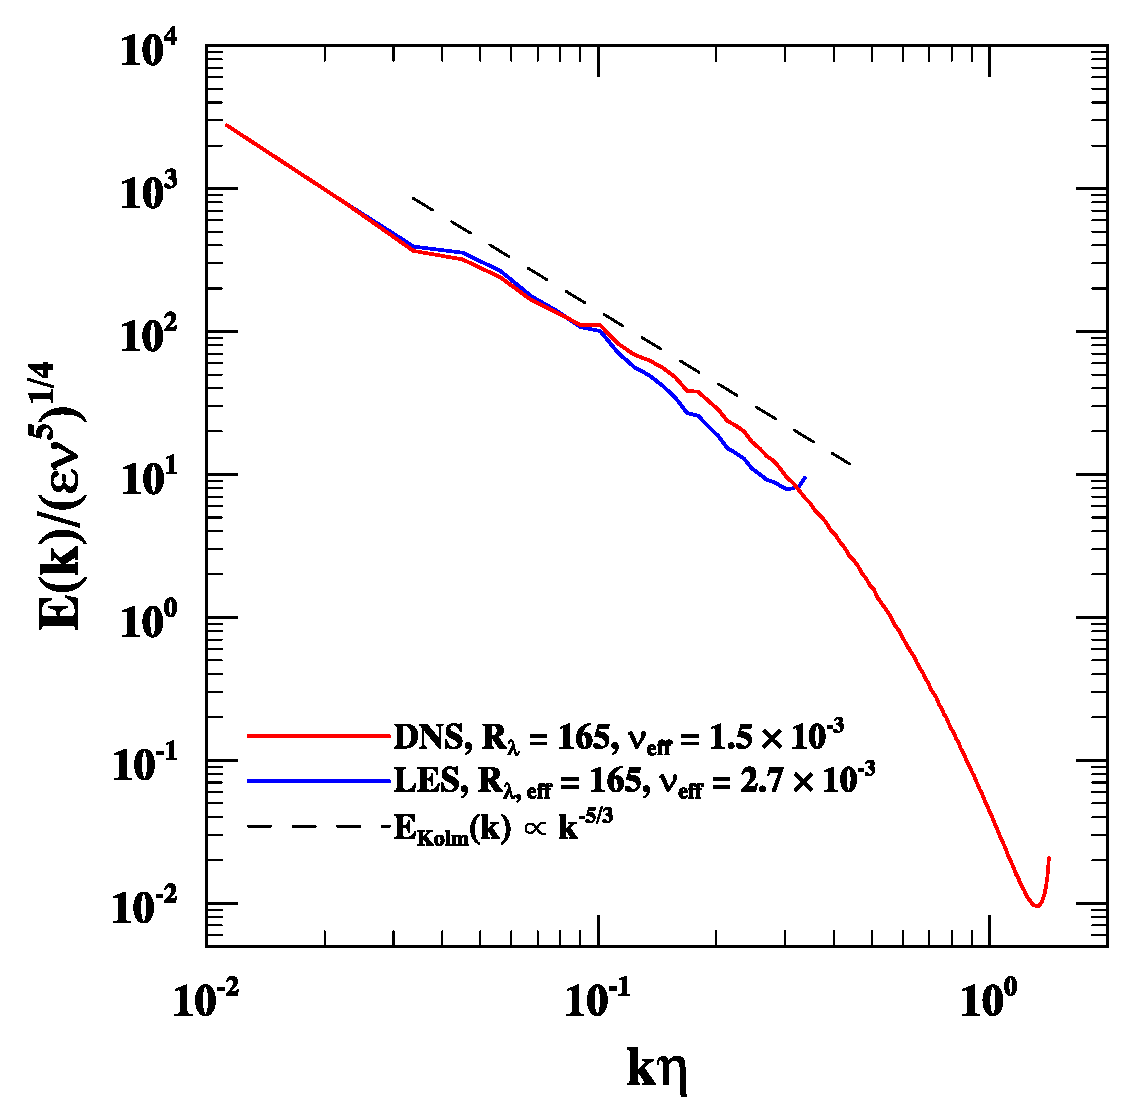
\includegraphics[width=8cm]{img/plots/2-1-2a-spec.pdf}
\caption{
The normalised energy spectra of background turbulent flows for both DNS and LES. Dashed line provides comparison with $k^{-5/3}$ curve of theoretical Kolmogorov spectrum (see Equation~\ref{eqn:kolm}) for inertial subrange.
}
\label{fig:spec}
\end{figure}

\begin{figure}[h]
\centering
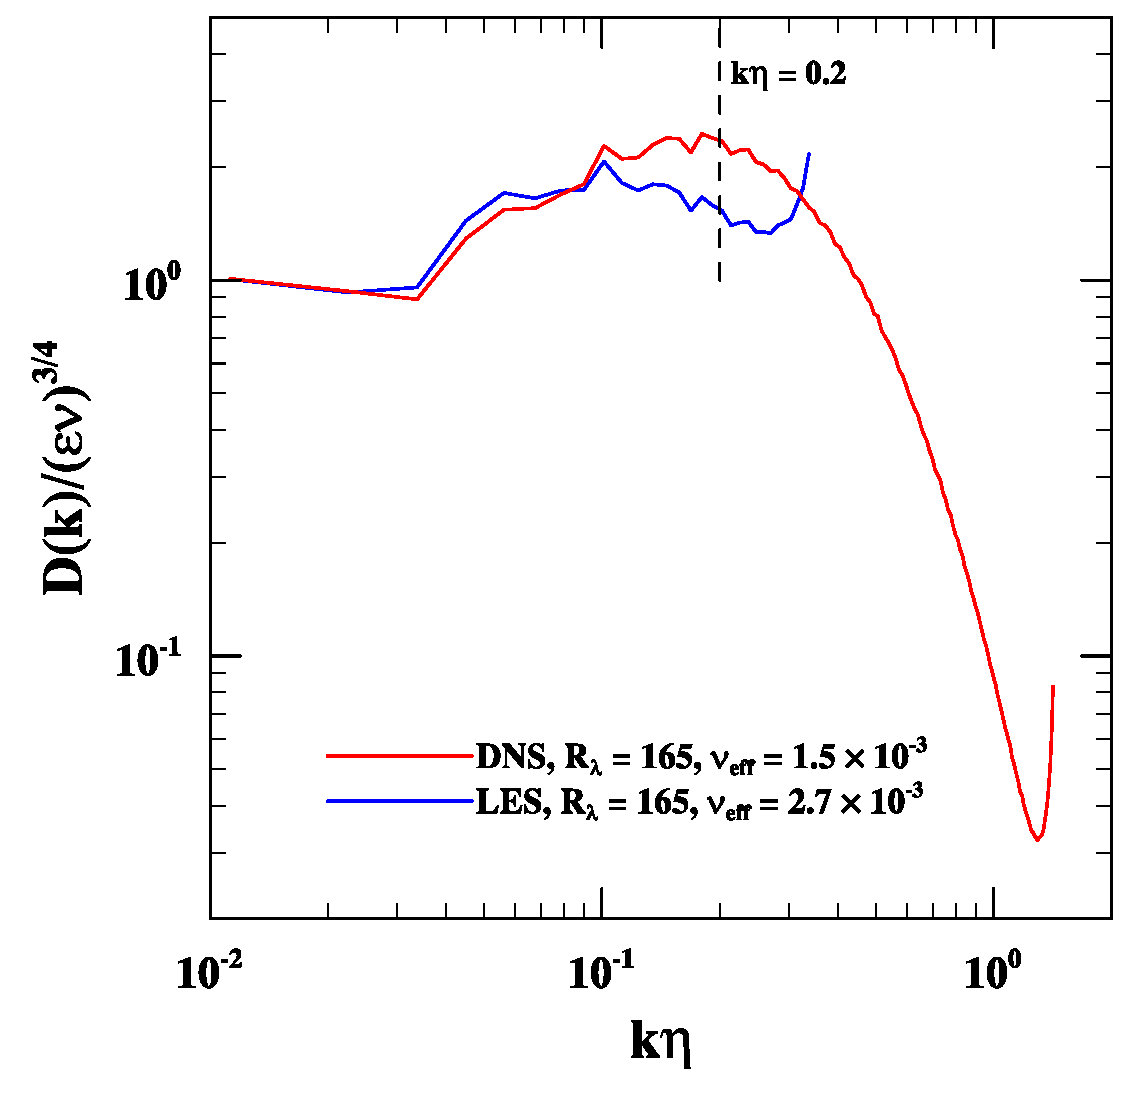
\includegraphics[width=8cm]{img/plots/2-1-2b-diss.pdf}
\caption{
The normalised energy dissipation spectra of background turbulent flows for both DNS and LES.
Point where $D(k)$ is expected to be maximal (for $k \eta = 0.2$) is marked by dashed line. 
}
\label{fig:diss}
\end{figure}

Figure \ref{fig:spec} clearly shows that both energy spectra follow theoretical Kolmogorov spectrum in the inertial subrange (reference line is shifted for clarity).
For LES, however, slight underestimation of the energy for intermediate wavenumbers may be observed.
This effect is~expected \parencite{Jin2010}, and it is attributed to the overdissipation of energy inherent in~the~spectral eddy viscosity model.
Such increase of dissipation rate for wavenumbers close to filtering threshold, $k_{c} = 30$, may be better observed on Figure \ref{fig:diss}, where respective dissipation spectra are shown.
It follows the region where $D(k)$ for LES is significantly smaller due to the smaller overall energy contained in these wavenumbers, since the energy is more strongly dissipated in larger modes (for $k \eta < 0.1$) due to contributions form the spectral viscosity.
This also leads to a shift in maximum of $D(k)$, which occurs for smaller wavenumbers than for DNS, where such peak occurs around $k \eta \approx 0.2$, that coincides with previous simulations and experimental results \parencite{Wang1993}.
Such discrepancies between DNS and LES in dissipation rates throughout inertial subrange may affect other properties of~turbulent flow, as well as particle collision statistics.
Another peculiar characteristic of~energy spectra is the sudden increase of energy for largest wavenumbers (close to $k_{\max}$ for DNS, or $k_{c}$ for LES).
\textcite{Rosa2017} observed similar artifacts, and suggested that they are due to accumulation of energy in the high-wavenumber modes, since the transport of energy is~limited there by the viscous suppression.



\subsection{Parameters of Particle-Laden Flows}
\label{ssc:ch2.flow.part}

When simulation of background turbulent flow reaches the statistically stationary state, as~described in Section \ref{ssc:ch2.flow.bstat}, individually tracked particles are introduced into the system with the uniform spatial distribution and inheriting velocity from the local fluid velocity.
In this study, we focus our interest on atmospheric clouds, where particles represent small water droplets (of radii ranging from $20$~$\upmu\text{m}$ to $60$~$\upmu\text{m}$) and the carrier fluid is atmospheric air.
These particles confine simulations to specific physical dimensions, where entire domain encompasses box with side length of approximately 33 cm.
Such conversion of spectral DNS units to physical units is based on matching the Kolmogorov scales.
In this study, we set: $\nu_{\text{air}} = 0.17 \, \text{cm}^{2} / \text{s} $ and $\epsilon_{\text{cloud}} = 400 \, \text{cm}^{2} / \text{s}^{3}$, which correspond to conditions observed in clouds with moderate to strong convection.
Note, that for the remainder of the thesis terms \emph{particles} and \emph{droplets} shall be used interchangeably.

For particle-laden flows, in general, the particle statistics are mainly functions of three independent nondimensional parameters.
Firstly, the particle inertia can be expressed in~terms of the \emph{Stokes number}, $St = \tau_p / \tau_k$, defined as the ratio of the inertial response time to the
Kolmogorov time scale.
Furthermore, the range of scales of turbulence in the system which affects particle behaviour is measured by \emph{Taylor-microscale Reynolds number}, $R_{\lambda}$, as defined in Section \ref{ssc:ch2.flow.bstat}, which (in OWC simulations) remains similar throughout all simulations (both DNS and LES) at approximately 165.
Finally, when settling particles are considered, we use \emph{normalised terminal velocity}, $S_V = V_T / v_k$, that is the particle still-fluid terminal velocity, $V_T$, normalised by the Kolmogorov velocity scale ($v_k = \eta / \tau_k$).
Note, that independence of~these parameters is true under simulations with one-way momentum coupling.
This picture becomes more complex with two-way coupling.
When effects of particles on the flow are taken into account, these parameters become indirectly dependent, e.g. large settling particles (with larger $St$ and $S_V$) are known to create additional vortex structures in flow, affecting $R_{\lambda}$, which -- in turn -- may alter settling velocity of particles (and, thus, $S_V$).

\begin{table}[h]
\centering
\small
\begin{tabular}{lrrrrrrrrr}
$\mathbf{a}$ [$\upmu\text{m}$] & 20 & 25 & 30 & 35 & 40 & 45 & 50 & 55 & 60  \\ \hline
$St$ & 0.254 & 0.396 & 0.571 & 0.777 & 1.015 & 1.284 & 1.585 & 1.918 & 2.283 \\
$S_V$ & 1.789 & 2.790 & 4.018 & 5.468 & 7.143 & 9.040 & 11.160 & 13.504 & 16.071 \\
$Fr$ & 0.81 & 3.08 & 9.21 & 23.23 & 51.76 & 104.93 & 197.44 & 349.77 & 589.54 \\
$\eta / a$ & 29.60 & 23.69 & 19.73 & 16.91 & 14.80 & 13.16 & 11.84 & 10.76 & 9.87 \\
$\Delta x_{\text{DNS}} / a$ & 64.58 & 51.67 & 43.06 & 36.90 & 32.29 & 28.70 & 25.83 & 23.48 & 21.53 \\
$\Delta x_{\text{LES}} / a$ & 219.62 & 175.70 & 146.42 & 125.50 & 109.81 & 97.61 & 87.85 & 79.86 & 73.21 \\
$\Delta t / \tau_p \times 10^2$ & 17.21 & 11.02 & 7.65 & 5.62 & 4.30 & 3.40 & 2.75 & 2.28 & 1.91 \\ \hline
\end{tabular}
\caption{Basic parameters for particle-laden flows corresponding to radii of particles (in $\upmu\text{m}$) used in this study.
$S_V$ and $Fr$ are only applicable to simulations with gravity.
For details of listed parameters, see text.
Note, that values of $\Delta x / a$ ratio are listed separately for DNS and LES, since their spatial step $\Delta x$ differ significantly due to much smaller density of grid points in LES without changing domain size. }
\label{tab:part-stats}
\end{table}

Such parameters for simulations in this study, depending on droplet radius, are presented in Table \ref{tab:part-stats}.
In addition, the Froude number, $Fr$, is defined as the ratio of particle response time to the residence time of the particles in a Kolmogorov eddy.
Its value, however, may be expressed in terms of basic parameters introduced above, since $Fr = St \cdot S_V^2$.
Properties of~general particle laden-flows are often dependent on density ratio of two phases, but due to~focus of this study on atmospheric phenomena, such ratio remains constant, as
$$
\frac{\rho_p}{\rho} 
= \frac{\rho_{\text{water}}}{\rho_{\text{air}}} 
= \frac{1 \, \text{g} / \text{cm}^3}{0.001 \, \text{g} / \text{cm}^3} 
= 10^3 .
$$
For a broader picture, an extended analysis concerning the influence of particle–fluid density ratio on the dynamics of finite-size particles in homogeneous
isotropic turbulent flows can be found in \textcite{Shen2021}.
Since the density ratio is fixed in this study, particle mass loading, $\Phi_m$, is exclusively used as a measure of relative amount of particles in a system as it is directly related to the volume fraction by $\Phi_V = \Phi_m \cdot 10^{-3}$ (see Section \ref{ssc:ch2.flow.part}).
On that note, also recall that in some cases, to obtain systems with larger mass loading, superparticle parameterisation was used, where single computational particle represents several physical particles.
For more information in which simulations superparticles were applied, see Appendix \ref{app:spp}. 

Table \ref{tab:part-stats} also includes some spatial and temporal ratios used as control parameters.
Relatively large values of $\eta / a$ and $\Delta x / a$ indicate that indeed particles used in these simulations are very small compared to both computational grid cells and smallest scales of turbulent eddies.
This second observation is paramount, as it not only makes the point-particle approximation justified, but also is of importance for simulations under two-way momentum coupling. 
All computations of the interphase momentum transfer use a simplified model under assumption that indeed $a \ll \eta$, and additional corrections are not necessary \parencite{Horwitz2016}.

\smallskip

Due to the influence of momentum transfer from particles to the fluid, some simulations under two-way momentum coupling required reduction of time step to preserve numerical stability of the simulation.
The base value used ($\Delta t = 9 \times 10^{-4}$) accounts for presence of~particles \parencite{Zhou2001}, adjusted to partially account for interactions between particles (as modelled by their hydrodynamic interactions), satisfying relation $\Delta t / \tau_p < 0.15$, where $\tau_p$ denotes particle response time, that was recommended by \textcite{Ayala2007}.
Only slight exceptions are simulations with the smallest droplets ($20$~$\upmu\text{m}$) where this ratio is $0.17$. 
Despite that, for some simulations $\Delta t$ needed to be further reduced, in same cases by a factor of $4$.
This was most common for simulations with settling particles and high super-particle factor, $M$, that often coincided with high particle mass loading.
These problems with stability seem to be caused by spikes in values of velocity field gradient that are inflated by momentum transfer from particles (i.e. $\mathbf{f}^{(p)}$ term in Equation \ref{eqn:n-s}), that locally saturates capabilities of~the~pseudo-spectral method (makes ''effective'' CFL much higher than required threshold of $0.3$) and destabilises entire simulation.

These issues require a separate, systematic treatment, but based on the experimental data obtained in this study (i.e. observation of cases where $\Delta t$ required adjustment) some initial observations may be put forward.
First of all, clearly, the risk of such oversaturation depends on the average number of particles per grid node, which clearly depends on total amount of~particles and their masses (radii), but also, in this case, used simulation method.
As outlined before, we employ LES to model turbulence with similar parameters as with DNS using higher grid resolution, but still populating it with the same number of particles.
On average, with grid sizes used here, it means that $64$ times more particles influence single node in LES than in DNS.
Moreover, this is exacerbated by preferential particle concentration (as measured by radial distribution function, see Section \ref{ssc:ch2.coll.rdfrrv}) that makes some nodes more saturated by particles than others.
For the same reason, using super-particle parameterisation (i.e. when $M > 1$) may introduce non-physical clustering, as single computational particle carries $M$ times more momentum.

This effect may be even more pronounced, as projection of particle momentum onto nearest neighbouring node depends on its distance to the position of that node.
For large values~of~$M$, much larger mass is concentrated at a single point, which may happen to be located very close to an actual node and impart its huge momentum contribution, causing affected node it to be oversaturated.
For smaller $M$ (or, preferably, $M=1$) particle mass should be more evenly distributed around node locations, making such occurrence statistically much less likely.
Finally, when the motion of particles is statistically anisotropic, and their velocity, on average, is larger in one particular direction, their contributions to the fluid motion are less likely to cancel each other and more likely to be amplified in that direction.
This is exactly the case of settling particles where gravity introduces such anisotropy, and it seems to explain why instabilities discussed here (and necessary reductions in $\Delta t$) were observed much more frequently for simulations with gravity.
These observations are purely qualitative, as deeper analysis of these issues were beyond the scope of this thesis.
Even though further study is~encouraged, due to complex nature of interactions between two phases in TWC simulations, it is difficult to predict whether simple criterion depending solely on $\tau_p$ can be established here, especially when additional parameterisations (LES, super-particles) are considered.



\subsection{Effects of Particles on Turbulence Modulation}
\label{ssc:ch2.flow.twc}

When statistics of turbulent flow (see Section \ref{ssc:ch2.flow.bstat}) are concerned, they remain unaffected by the presence of particles in the system, unless two-way momentum coupling is included.
In~case of TWC simulations, such effects are observed, and are usually referred to as \emph{turbulence~modulation} due to particles.
Such effects were systematically studied for DNS in \textcite{Rosa2020}.
In this section, similar range of results is presented, this time including also these obtained using LES.
The comparison of LES and DNS results may be particularly illuminating, since most of momentum transfer from the fluid to particles is usually attributed to~the~smallest scales of vortical structures, and these depend on the quality of subgrid-scale model parameterisation in LES.
This is especially true for smaller particles, since their dynamics is mainly governed by fine turbulent structures. 
For more involved discussion on the physical interpretation of these results, see \textcite{Rosa2020}.
Here, the focus is on the comparison of already established results from DNS with those obtained in this study using LES method.

\begin{figure}[h]
\centering
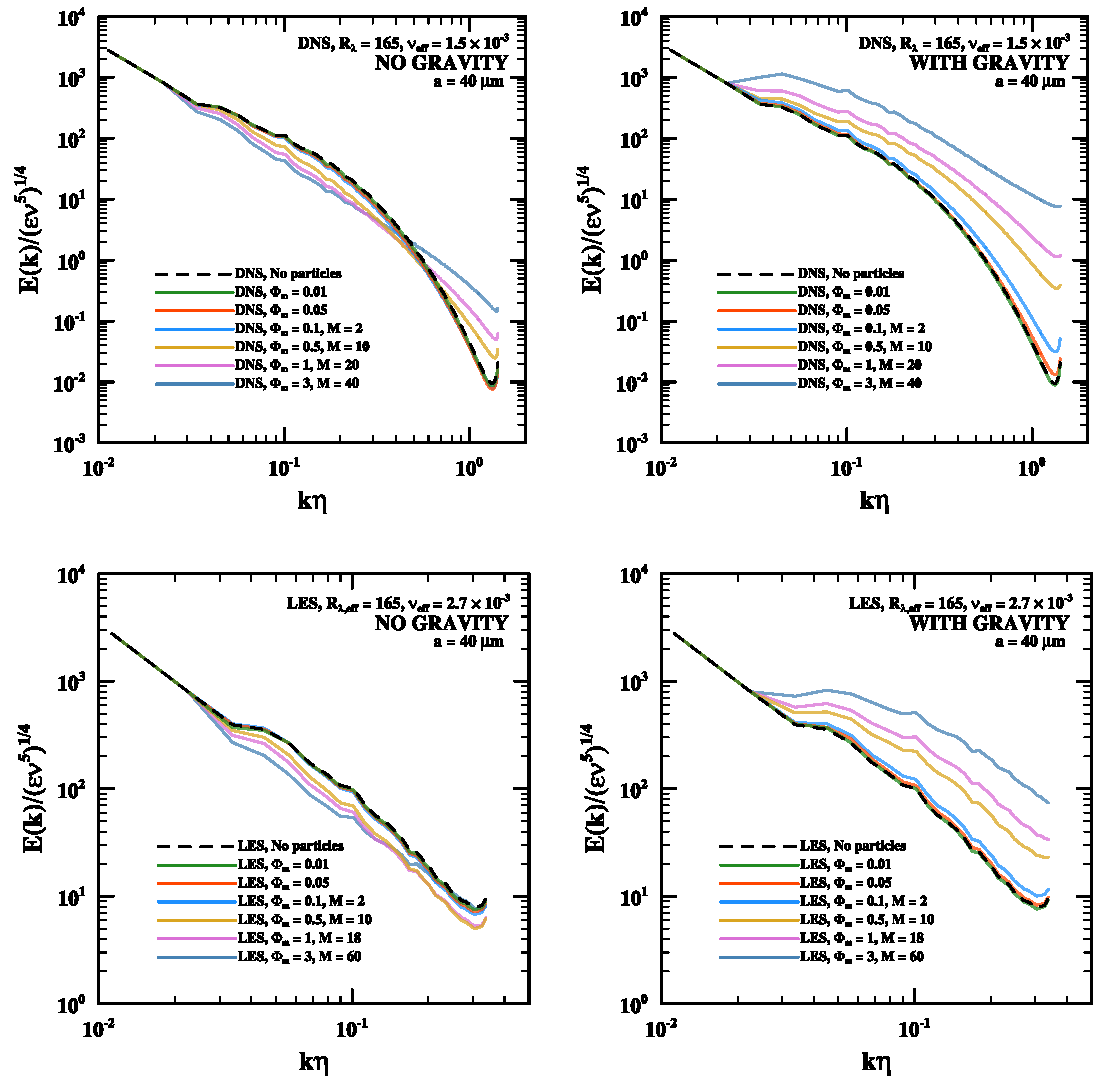
\includegraphics[width=13.5cm]{img/plots/2-1-4a-modspec.pdf}
\caption{
The normalised energy spectra of turbulent flows with droplets of radii $40$~$\upmu\text{m}$, with and without gravity, as obtained using both DNS and LES with two-way momentum coupling and different particle mass loadings.
Dashed lines represent spectra without turbulence modulation by particles (see Figure \ref{fig:spec}). For comparison (with DNS results only), see \textcite[Figure 4]{Rosa2020}.
}
\label{fig:modspec}
\end{figure}

\begin{figure}[h]
\centering
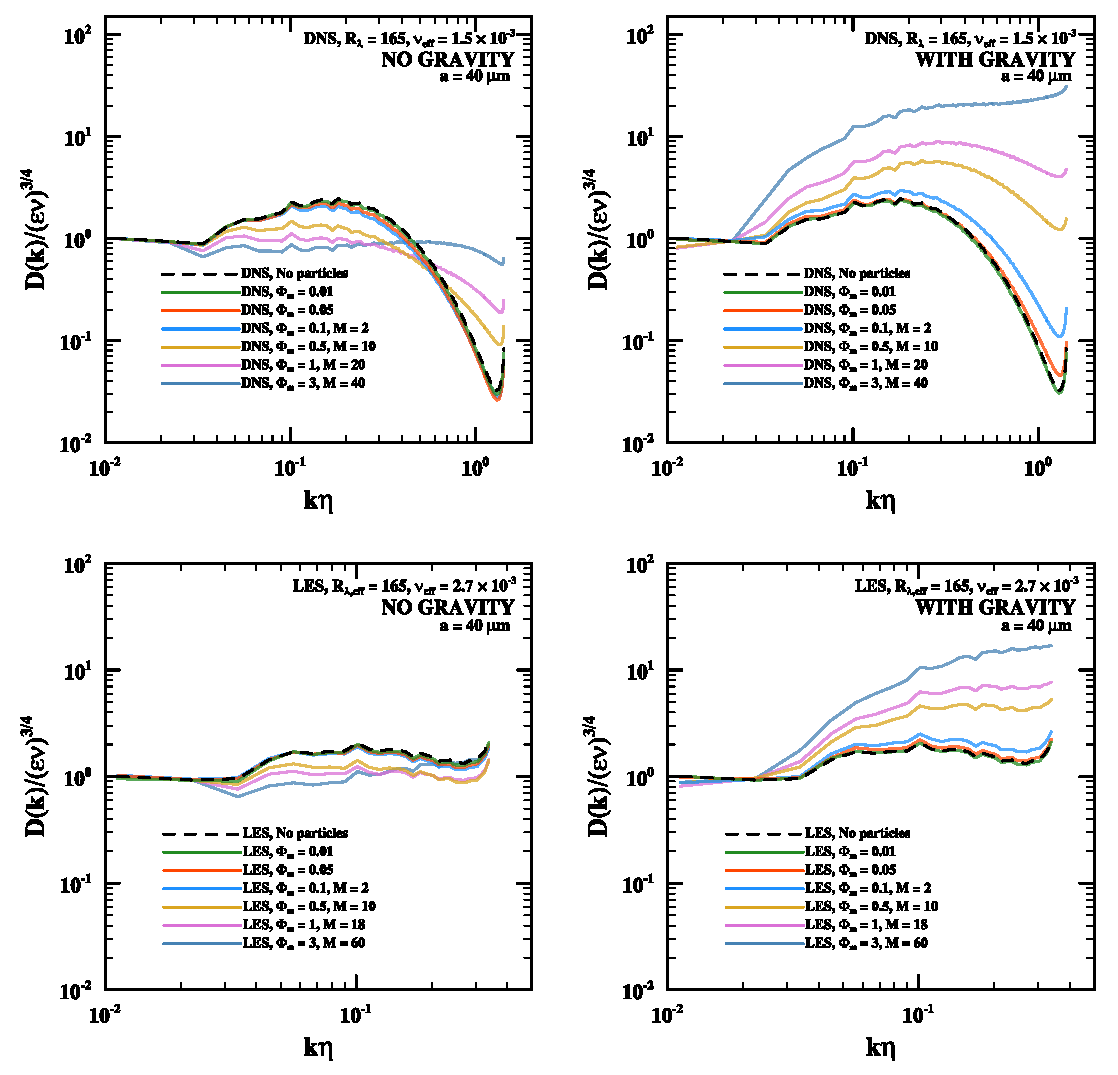
\includegraphics[width=13.5cm]{img/plots/2-1-4b-moddiss.pdf}
\caption{
The normalised energy dissipation spectra of turbulent flows with droplets of radii $40$~$\upmu\text{m}$, with and without gravity, as obtained using both DNS and LES performed under two-way momentum coupling with different particle mass loadings.
Dashed lines represent dissipation spectra~without turbulence modulation by particles (see Figure \ref{fig:diss}). For comparison (DNS only), see Figure 5 in \textcite{Rosa2020}.
}
\label{fig:moddiss}
\end{figure}


Figures \ref{fig:modspec} and \ref{fig:moddiss} show effects of particles in TWC simulations on energy and dissipation spectra of the underlying turbulent flow.
All simulations were performed with particles with radius of $40$~$\upmu\text{m}$, and with varying mass loadings, $\Phi_{m}$, that measure the amount of particles present in the system.
Reference spectra from simulations without two-way coupling were provided with dashed black lines.
Results for DNS (top plots) show agreement with corresponding results in \textcite[Fig.4 and 5]{Rosa2020}.
Moreover, in this study data from simulations with higher mass loading is presented (there, it was limited to $\Phi_m = 0.747$), and~in~all~cases trends that were already observed continue further with increase in $\Phi_m$.

Results of LES show promising alignment with those from DNS.
It is important to recall that energy and dissipation spectra are directly available for smaller range of wavenumbers in LES, which coincides with part of DNS spectrum for approximately $k \eta < 0.25$.
For non-settling particles, this is the part of energy and dissipation spectra in DNS that decrease with increasing mass loading, and it is also reflected in results for LES.
Similarly, when effects of gravity are included, sharp increase in both spectra throughout all modes (for $|\mathbf{k}| > 2$) is~witnessed, as expected.

The dual influence of TWC on energy spectrum for non-settling particles is known as ''pivoting'' \parencite{Squires1990,Bosse2006,Rosa2020}.
The kinetic energy of fluid is suppressed for intermediate wavenumbers due to increased energy dissipation, while it is increased for high wavenumbers due to combined effects of larger viscous dissipation and transfer of momentum from the particles to the fluid.
The increase of energy for small turbulent scales cannot be adequately represented in LES, in part due to the fact that used subgrid-scale model is agnostic to any momentum transfer form particles. 
Similar remarks are valid for the settling particles, but here increase due to transfer of momentum from particles is larger and present throughout wide range of wavenumbers, and such transfer affects even intermediate turbulent scales that are directly resolved in LES.

\begin{figure}[h]
\centering
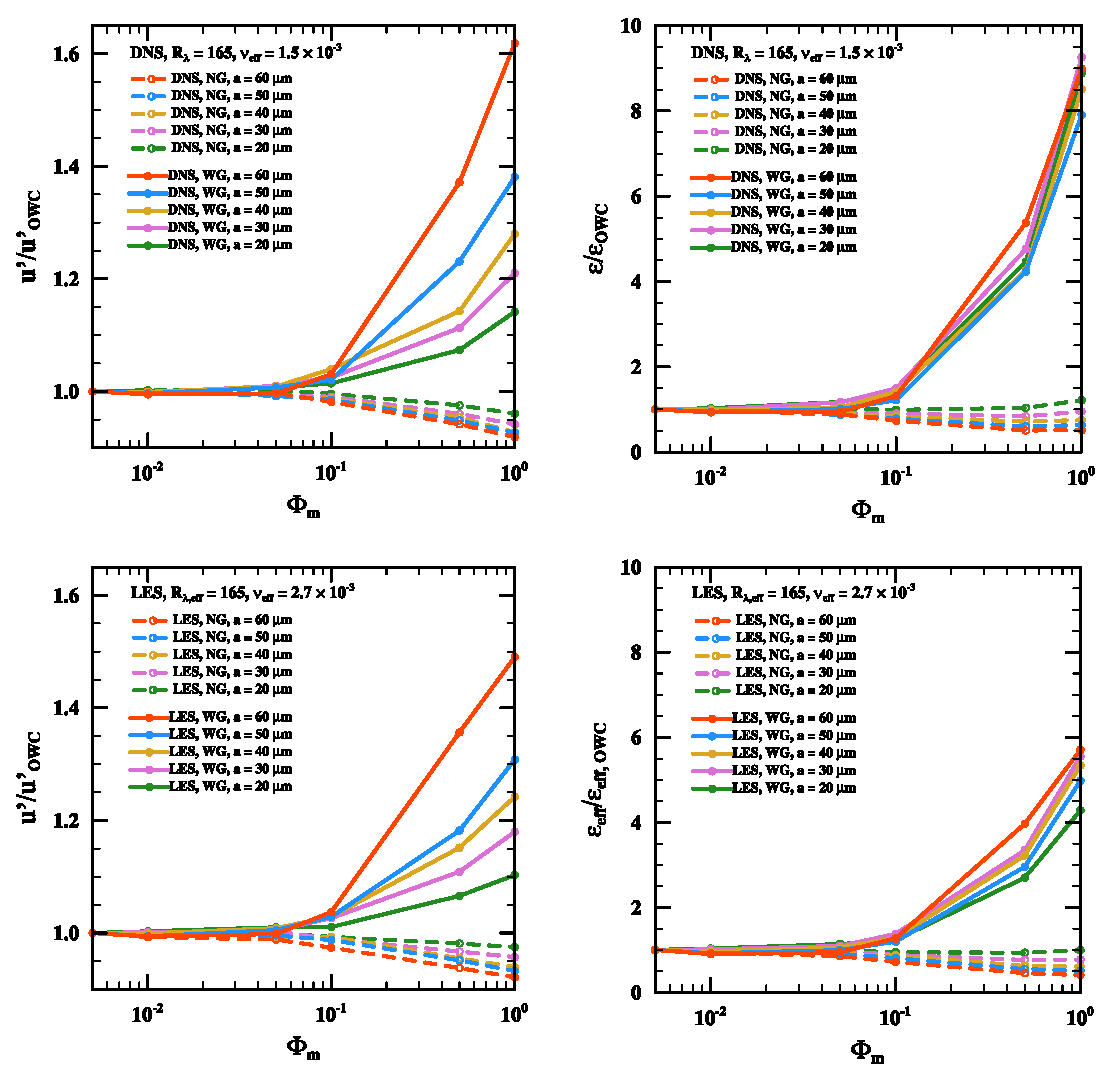
\includegraphics[width=13.5cm]{img/plots/2-1-4c-modstat.pdf}
\caption{
Time averaged statistics of turbulent flows as obtained by DNS and LES under two-way momentum coupling, normalised by the corresponding statistics from simulations without turbulence modulation (OWC).
Plotted statistics include, the effective energy dissipation rate, $\epsilon_{\text{eff}}$ (top figures for DNS and LES, respectively), and the rms fluctuating velocity, $u'$ (bottom figures, likewise).
WG denotes simulations with gravity (continuous lines); NG -- without gravity (dashed lines).
For comparison (DNS only), see Figure 11 in \textcite{Rosa2020}.
}
\label{fig:modstat}
\end{figure}

In addition to aforemontioned spectra, Figure \ref{fig:modstat} shows impact of turbulence modulation on two specific statistics, i.e. rms fluctuating velocity and energy dissipation.
Results are normalised using respective statistic for simulations without two-way coupling, and plotted depending on the particle mass loading and for five different droplet radii, both with and~without effects of gravity.
These results may be compared with those presented in \textcite[Fig. 11]{Rosa2020}, although mind difference in setup and scaling of x-axis, that is responsible for different outlook of plotted data.

We can easily see that both statistics are increasing with $\Phi_m$ for settling particles, while in the absence of gravity the effect is opposite.
Also trends in $u'$ and $\epsilon$ are somewhat expected, as both of these statistics are related to the total kinetic energy of turbulence ($u' \propto \sqrt{E}$).
In particular, for settling particles, the steep increase of both statistics with particle mass loading may be explained by larger fluid velocity gradients caused by the fast settling particles.
Also note, that due to different way of plotting results (relative to $\Phi_m$ and not number of particles), we may also observe that $u'$ is much more dependent on radii of individual droplets, while $\epsilon$ is much less sensitive to that, and seems to be mainly driven by the particle mass loading in the system.
This difference may be seen in results for both DNS and LES.

On that note, again, we can observe qualitative agreement of statistics for both DNS and~LES.
Same trends can be seen in both cases.
When actual magnitudes are concerned, values of $u'$ are surprisingly close for both methods, although slightly underestimated in case of LES.
This effect may be due to smaller sensitivity of coarser LES grid to the creation of vortical structures by large inertial particles with high settling velocity, that is responsible for increase in magnitude of turbulence, as measured by $u'$.
These vortices are more likely to be induced on smaller scales, and subgrid-scale model has no knowledge of such preferable conditions. 
 
Much more significant discrepancies can be observed in case of energy dissipation.
For~LES, effective value was taken, but still they were approximately two times lower than those obtained by LES.
These differences may be partly explained by the fact that $u'$ is independent from numerical viscosity, while $\epsilon$ is not, and it may be affected in estimating ``effective'' viscosity including contribution of the modelled spectral viscosity.
Also inspection of dissipation spectra (and $\epsilon$ is defined as its integral) shows that, even though it is consistently adjusted in LES for modes that are directly resolved, 
dissipation for settling particles is still significantly boosted even for the largest wavenumbers.
This increase cannot be fully accounted for in LES and contributions of subgrid-scale model (which is agnostic of any momentum transfer from particles) are not enough to make up for that unresolved modes.

Taking all above observations into considerations, LES shows initial promise in properly representing statistics of background turbulent flow, even when influence of two-way momentum coupling is present.
Still, it is important to be aware of its limitations, and lack of directly resolved smaller scales that may impact some properties of turbulent flow more than another.
Also, it introduces discussion of the quality of chosen subgrid-scale model, and whether development of a model that would be sensitive to momentum transfer form particles is viable to alleviate some of observed limitations of LES in this context.



\section{Kinematic and Dynamic Collision Statistics of Particles}
\label{sc:ch2.coll}

In many cases the effects of turbulent flow on certain statistics of particles are more important than properties and statistic of the underlying flow itself, whether inherent or modulated by~the~presence of particles.
In atmospheric sciences, for example, modelling of the behaviour of cloud droplets is of paramount importance to better understand mechanisms that are involved in formation of precipitation or other phenomena.
We may consider single-particle statistics, which describe properties of particles that are not directly dependent on other particles in its vicinity, such as its settling velocity under the effects of gravity.
Here, however, we focus our attention on two-point particle statistics, which measure behaviour of~particles in relation with each other.
More precisely, we shall explore collisional statistics, i.e. ones that involve particles at contact distance, i.e. when their distance is no larger than sum of~their radii.
First two of these, i.e. the RDF and the RRV introduced in the next section, are used to describe relative concentration and motion of particles, thus are commonly referred to as~\emph{kinematic} statistics. 

\smallskip

\subsection{Radial Distribution Function and Radial Relative Velocity}
\label{ssc:ch2.coll.rdfrrv}

The \emph{radial distribution function} (RDF) may serve as a measure of preferential concentration of particles.
The \emph{radial relative velocity} (RRV) is a way to quantify average relative velocity of particles.
Both of these statistics are important, as they may serve to evaluate collision rate of particles in given system.
They both were introduced for that very purpose by \textcite{Sundaram1997}, based on related concepts developed in statistical mechanics.

We assume that we are dealing with monodisperse system, with particles of radius $a$.
For~bi- or poly-disperse systems the RDF at contact is close to unity.
This is because droplets of different inertia occupy different regions of the turbulent flows.

The RDF at contact distance (i.e. for $r = R = 2a$) may be effectively computed during simulation using its definition as proposed by \textcite{Wang2000,Zhou2001}.
In~general, for any distance $r$ from each particle, we consider spherical shell with inner and outer radii equal to $r - \delta r$ and $r + \delta r$, respectively, where $\delta$ is a small fraction ($\sim 0.01$) of~contact distance $R$.
Its volume may be expressed by $V_s = 4 \pi [(r + \delta)^3 - (r - \delta)^3)] / 3$.
Also, by $N$ we shall denote the total number of particle pairs, which is equal to $N_{\text{part}}(N_{\text{part}} - 1) / 2$, and by $N_s$ the total number of particle pairs detected with their separation distance, $r$, that falls into spherical shell defined as above.
Then, the RDF for distance $r$ at given time $t$ is defined as: 
\begin{equation}
g_{11}(r; t) = \frac{N_s / V_s}{N / V} ,
\label{eqn:rdf}
\end{equation}
where $V$ is the volume of entire computational domain.
It may be further averaged over time to obtain estimate of $g_{11}(r)$.

To compute the RDF at contact distance, the simplest way would be to just evaluate it~for~$r = R$.
This method, however, was found to be highly susceptible to numerical uncertainties, especially when particle concentration is relatively low.
Alternatively, we may use well established fact that for small separation distances ($r < \eta$) function $g_{11}(r)$ follows a power-law dependence with respect to $r$, with exponent that depends on $St$ and $S_V$ \parencite[Equation 11]{Rosa2013}.
Thus, we may calculate RDF using Equation \ref{eqn:rdf} for a range of distances, and then fit results into exponential function, in order to obtain more accurate estimate of $g_{11}(r = R)$.
In practice, similar procedure as in \textcite{Rosa2013} was employed, where distances from range between $R$ and $10R$ were divided into 180 discrete bins (shells) used for function fitting using least-squares method.
In general, for all collision statistics presented in this chapter, the estimates show that statistical uncertainties do not exceed $3 \%$.

\begin{figure}[h]
\centering
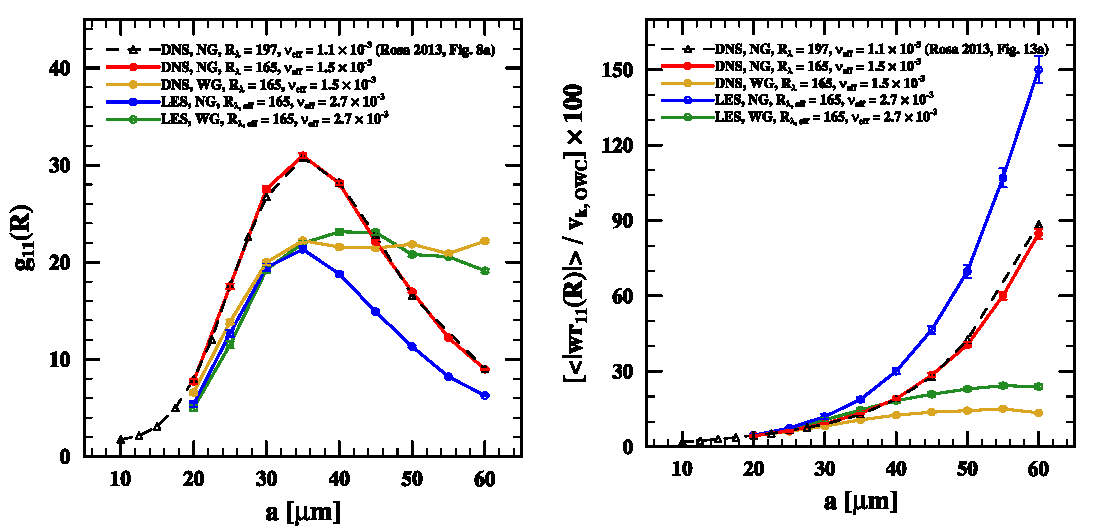
\includegraphics[width=13.5cm]{img/plots/2-2-1-owcrdfrrv.pdf}
\caption{
The values of the radial distribution function (RDF, left) and the radial relative velocity (RRV, right) at contact distance for simulations with one-way momentum coupling.
Results include data from both DNS and LES simulations, without (NG) and with gravity (WG).
}
\label{fig:owcrdfrrv}
\end{figure}

In figure \ref{fig:owcrdfrrv} (left), values of the RDF at contact distance obtained from simulations under one-way momentum coupling are shown for both DNS and LES, with and without gravity.
For comparison, results for DNS without gravity from \textcite{Rosa2013} are shown, and are perfectly matched to results obtained in this study.
Also previous observations are confirmed, where clustering of non-settling droplets (as measured by the RDF) is strongest for radii of $30-40$~$\upmu\text{m}$, i.e. in cases where the Stokes number is closest to $1$.
For smaller and larger particles values of the RDF fall off quite rapidly.
For much smaller $St$ particle behave more and more as fluid elements, while for much larger $St$ they become massive enough to be barely impacted by fluid, which manifests in much less turbulent clustering, thus the RDF is expected to approach $1$ in those two limits.
In case of settling particles, relatively smaller values of the RDF are attained, but the influence of gravity causes the RDF to not drop rapidly for larger particles, but remain at the same peak level attained for particles with $a \approx 35$~$\upmu\text{m}$. 
This effect is attributed to tendency of heavier particles to accumulate in the downward flow regions, forming elongated (filament-like) structures \parencite{Rosa2015}. 

When gravity is not considered, the results of LES significantly underestimate the RDF, including peak values around $St=1$ being reduced by approximately $60 \%$ \parencite{Fede2006,Yang2008,Marchioli2008}.
This difference may be attributed to filtering of~small-scale turbulence which has significant impact on concentration of particles of that size.
On the other hand, LES is confirmed \parencite[see][]{Rosa2017} to be much more accurate in predicting the RDF of settling particles.
In general, it is argued that heavy settling particles due to increased velocity in the direction of gravity vector spend less time interacting with turbulent eddies and more uniformly sample the flow \parencite{Ireland2016}.
This manifests, in general, in reduced clustering due to turbulence (lower RDF) for settling particles, irrespective of method used.
This also explains why LES is much more accurate in~this~case, as filtered scales of turbulence have much more limited impact on particles, then in case of no gravity.

\smallskip

In case of the relative radial velocity, methodology used in its computation is similar to~the~RDF, since comparable power-law relation also exists \parencite[Equation 13]{Rosa2013}.
For any two particles with separation vector $\mathbf{r}$ and relative velocity $\mathbf{w}$ we define their \emph{radial relative velocity} as:
\begin{equation}
w_r = \mathbf{w} \cdot \frac{\mathbf{r}}{|\mathbf{r}|} ,
\label{eqn:rrv}
\end{equation} 
i.e. dot product of relative velocity with direction vector of their separation.
Note, that $w_r$ is largest for two particles speeding towards each other.
Relative velocities are averaged within shells and fitted into exponential function in a similar fashion as with the RDF.
Then, they are averaged over time, to obtain $\langle|w_{r, 11}(r = R)|\rangle$, and finally normalised using the Kolmogorov velocity scale, $v_k$, to make resulting value dimensionless.

Corresponding results of the RRV for simulations with one-way momentum coupling are presented in Figure \ref{fig:owcrdfrrv}.
When effects of gravity are not considered, the RRV monotonically increases with particle radius and such increase is close to exponential.
This is due to increasing contributions from large-scale turbulent motion and other non-local contributions.
The~picture becomes more complicated for settling particles.
We may distinguish regime of~light particles, up to $30$~$\upmu\text{m}$, where the RRV is independent of effects gravity and assumes very similar values to these obtained without accounting for gravity (\emph{gravity-independent interaction}).
This changes for heavier particles, whose settling velocity is larger which reduces residence time of particles in large-scale turbulent eddies, and similar accumulation of large-scale motion cannot happen, as for non-settling particles (\emph{gravity-modulated interaction}).
Also, as previously mentioned, heavier particles tend to arrange into downward-flowing filament-like structures, which are characterised by much more velocity correlation, thus reducing the RRV.
This reduction gets stronger with increasing radius of particles, slowing increase of the RRV until it reaches maximum, location of which is dependent of $R_{\lambda}$ \parencite{Rosa2013}, which happens here around $a = 50$~$\upmu\text{m}$.
Then, further reduction causes the RRV to decrease with particle size, as heavy particles become fast enough to neglect most of the influence of~turbulence on their relative velocities.

The results of LES show reverse tendency than for the RDF, and they are consistently overestimated by approximately $60 \%$ in comparison with DNS.
This effect may be attributed to the lack of filtered small-eddies that introduce more variance in particle motion.
In the absence of such disturbances, particles align more with large-scale eddies, and effects that cause rapid growth of the RRV with particle size are not only present in LES but are magnified, resulting in the increased RRV.
This is still valid for settling particles, yet similar effects are present as in DNS that reduce the RRV.
For that reason, even though overblown in~absolute value, the RRV for LES follow the same trends and the ratio of corresponding values, surprisingly, remains close to constant, especially for $a > 40$~$\upmu\text{m}$.     


\subsection{Dynamic and Kinematic Collision Kernels}
\label{ssc:ch2.coll.gamma}

The final particle-pair statistic introduced here is the \emph{collision kernel}, which is the ratio of~the~number of occurrences of particle collisions to the total number of particle pairs.
In~general, such kernel is expressed as a symmetric matrix, $\mathbf{\Gamma}(t)$, where entries correspond to ratios of collisions between particles with different properties (usually sizes, radii).
Here, we consider systems that are monodisperse, hence it reduces to single scalar quantity $\Gamma_{11}(t)$.
This~statistic is of utmost importance, especially when atmospheric sciences is concerned, as ratio of droplet collision is important for many processes in cloud microphysics, such as droplet collisional growth and coalescence, which is the driving factor in formation of precipitation.   

The collision kernel may be arduously computed by tracking all collision events in the system and normalising it by the number of all possible particle pairs.
Such value is referred to as the \emph{dynamic collision kernel} and denoted by $\Gamma^D_{11}(t)$, or just $\Gamma^D_{11}$ when averaged over~time.
Statistical uncertainty of such process is calculated as in \textcite[Equation 17]{Rosa2013}.
An~alternative formulation is the so-called \emph{kinematic collision kernel}, $\Gamma^K_{11}{t}$, based on \textcite{Sundaram1997}, where it is defined as a function of kinematic statistics computed in~previous section, and expressed by:
\begin{equation}
\Gamma^K_{11} = 2 \pi R^{2} \langle | w_{r, 11}(r = R) | \rangle g_{11}(r = R),
\label{eqn:gamma-k}
\end{equation}
where $r$ is the separation distance between particles and $R = 2a$.
Note that values or both kernels are expected to be in almost perfect agreement (up to statistical uncertainties), and presented simulation result confirm that expectation.

\begin{figure}[h]
\centering
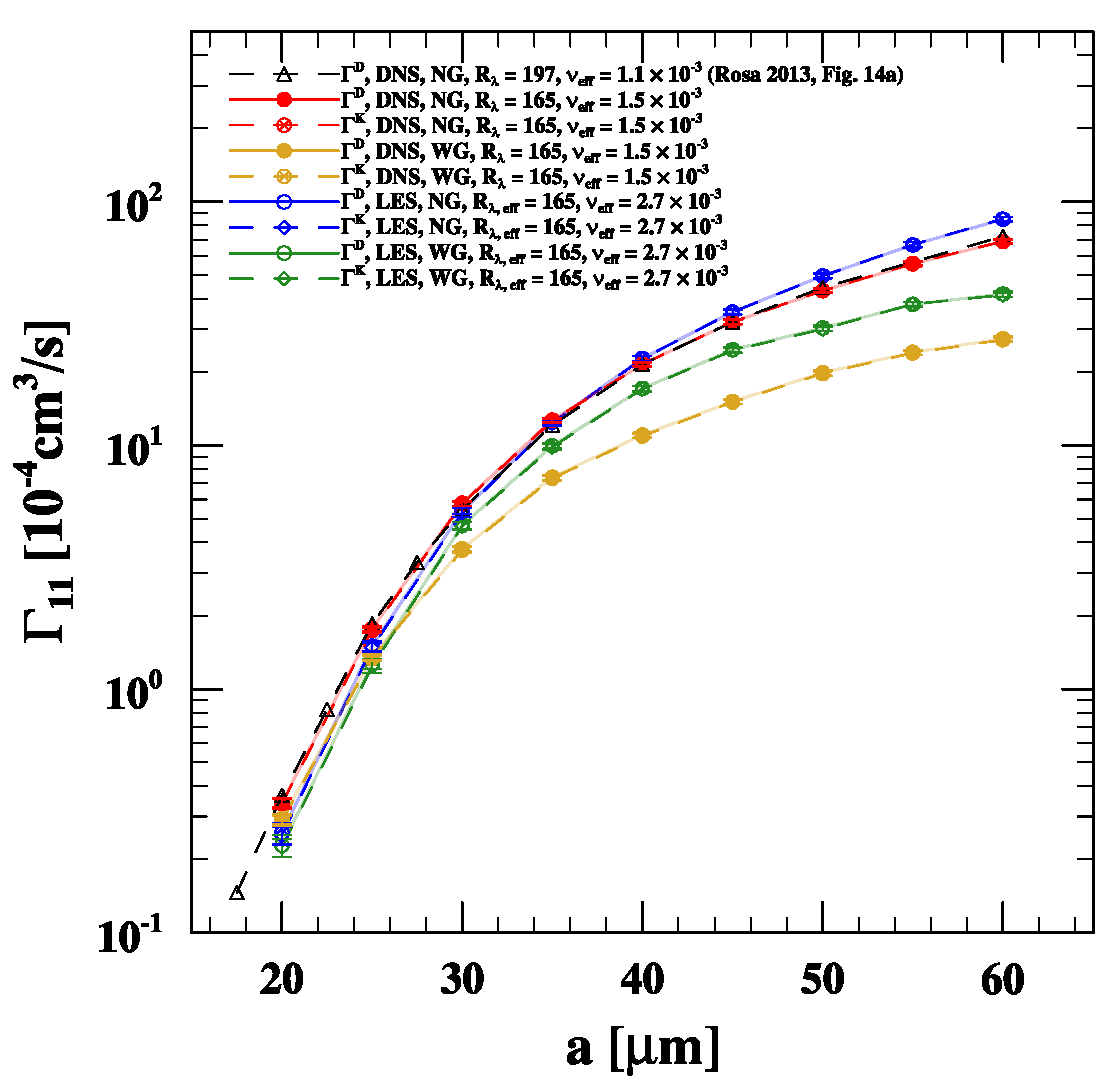
\includegraphics[width=10cm]{img/plots/2-2-2-owcgamma.pdf}
\caption{
The values of both dynamic and kinematic collision kernels for simulations with one-way momentum coupling.
Results include data from both DNS and LES simulations, without (NG) and with gravity (WG).
Continuous lines represent values for dynamic kernel ($\Gamma_{11}^D$), and dashed ones (almost overlaid on continuous ones due to their agreement) -- for kinematic kernel ($\Gamma_{11}^K$). 
}
\label{fig:owcgamma}
\end{figure}

The values of collision kernels for simulations under one-way momentum coupling are shown in Figure~\ref{fig:owcgamma}.
The results for dynamic kernel are plotted using continuous lines, and for the kinematic kernel dashed lines are used.
The data obtained for the RDF confirms previous observations that gravity leads to reduction of collision kernel by the factor of $2$ to $3$ \parencite{Rosa2013}.
Based on kinematic formulation, we may attribute that difference to the lower RDF for smaller settling particles ($a  < 40$~$\upmu\text{m}$), and for larger particles ($a  > 40$~$\upmu\text{m}$) rapid growth of the RRV for non-settling particles, as compared to reduced relative velocity in gravity-modulated interaction regime.
Nonetheless, discrepancies between collision kernels for settling and non-settling particles quickly diminish with smaller radii, and for small enough particles ($a < 40$~$\upmu\text{m}$) effects of gravity on $\Gamma_{11}$ may be considered negligible.

When results of LES are concerned, they compare very differently with DNS depending on whether we include gravity.
When gravity is not considered, collision kernels provided by DNS and LES are in quantitative agreement.
This may be explained by the values of the RDF and the RRV, which are, respectively, underestimated or overestimated by approximately the same relative amount.
This is due to filtering of small-scales eddies that increase turbulent concentration but also make large-scale flow motion of fluid more prominent increasing the RRV.
These two effects seem to cancel each other, when the particle collision rate is concerned, bringing both values close.
Different picture presents itself for settling particles.
For smaller particles ($a < 30$~$\upmu\text{m}$) differences in collision kernels are in quite good agreement.
For smallest radii concerned, LES even tends to overestimate the collision kernel, as the RDF is similar and the RRV is slightly overestimated in LES.
Nonetheless, absolute differences of $\Gamma_{11}$ are rather negligible for such low inertia particles.

On the other hand, for particles with radii larger than $30$~$\upmu\text{m}$ the difference between DNS and LES grow significantly.
This may be explained by the fact that LES correctly predicts the RDF of more massive particles, while still overestimating the RRV as for smaller ones.
This~leads to similar difference in $\Gamma_{11}$ as in the RRV, and no cancellation as in case of non-settling particles occurs.
The closer inspection of the RDF for LES with gravity shows that it may consistently decrease for particles with $a > 50$~$\upmu\text{m}$, but it cannot be confirmed by available data, and previous studies \parencite{Rosa2017} show that it may not be likely.
But if that is so, such reduction of LES error may eventually happen for particles massive enough.
Moreover, it may be observed that difference between LES and DNS starts to diminish when $a = 60$~$\upmu\text{m}$.
Still, such discrepancy in prediction of collision rate of larger settling particles between DNS and LES is considerable and should be further investigated.


\subsection{Collision Statistics in Simulations under Two-Way Momentum Coupling}
\label{ssc:ch2.coll.twc}

In previous sections, basic notions of collisional particle statistics were introduced, as well as methods of their computation with reproduction and short discussion of results obtained in~simulations under one-way momentum coupling.
Here, we shall present estimates of these statistics using simulations with two-way momentum coupling.
Similar results for DNS were recently presented and systematically analysed by \textcite{Rosa2020,Rosa2022}, but no such study were performed with LES.
For that reason it shall focus on comparison between results obtained by DNS and LES.

The results are presented for both kinematic statistics (RDF, RRV) and collision kernels.
Note that values of both dynamic and kinematic kernels were confirmed to be in quantitative agreement within statistical uncertainty, hence only data for dynamic kernel is shown.
Three types of plots are used to showcase influence of two-way momentum coupling on these statistics.
Firstly, they are plotted for selected fixed values of $\Phi_m$ depending on particle radii (see Figures \ref{fig:twcrdf}, \ref{fig:twcrrv}, and \ref{fig:twcgamma}; top row).
These may be considered an extension of plots from Sections \ref{ssc:ch2.coll.rdfrrv} and \ref{ssc:ch2.coll.gamma}, since they also contain similar curves shown for OWC simulations, extended by additional ones that involve TWC with increasing mass loading.
Remaining plots show droplet statistics for two radii ($30$~$\upmu\text{m}$ and $40$~$\upmu\text{m}$), chosen to represent particles most affected by turbulence (i.e. with $St \sim 1$), depending on the amount of particles in the system.
Plots in the bottom row of Figures \ref{fig:twcrdf}, \ref{fig:twcrrv}, and \ref{fig:twcgamma} are limited to relatively small particle content (up to 20 million; equivalent to $\Phi_m \approx 0.15$ for $a = 40$~$\upmu\text{m}$).
The values obtained from OWC simulations are included for reference on the leftmost edge of the plot (i.e.~$0$~on~the~$X$-axis). 
Results from simulations with broader range of mass loadings are shown in Figures \ref{fig:twcrdf}, \ref{fig:twcrrv}, and \ref{fig:twcgamma}.
Simulations where super-particle parameterisation was used (i.e. $M>1$) are explicitly marked by dashed line.
For more information pertaining to simulations with super-particle parameterisation and what exact values of $M$ were used, see Appendix \ref{app:spp}.
Results without effects of gravity are shown on the left, and those for settling particles - on the right. 

\medskip

\emph{Radial Distribution Function (RDF)}

Figures \ref{fig:twcrdf} and \ref{fig:twcrdfext} show results for the RDF.
The RDF for non-settling particles clearly exhibits similar dependence on particle size as in case of OWC, but its absolute value is~reduced with the increase of mass loading.
When effects of gravity are considered, the RDF is generally boosted in TWC for the smallest range of particles ($\sim 20$~$\upmu\text{m}$), while it becomes smaller with increasing particle radius and mass loading, reaching plateau for heavier particles.
These results for DNS are confirmed by \textcite[Fig. 19]{Rosa2020}, where dependence on particle size is more clear due to more results obtained for different droplet radii.
Furthermore, they are extended for larger mass loadings (0.5, 1) not present in previous studies.

\begin{figure}[h]
\centering
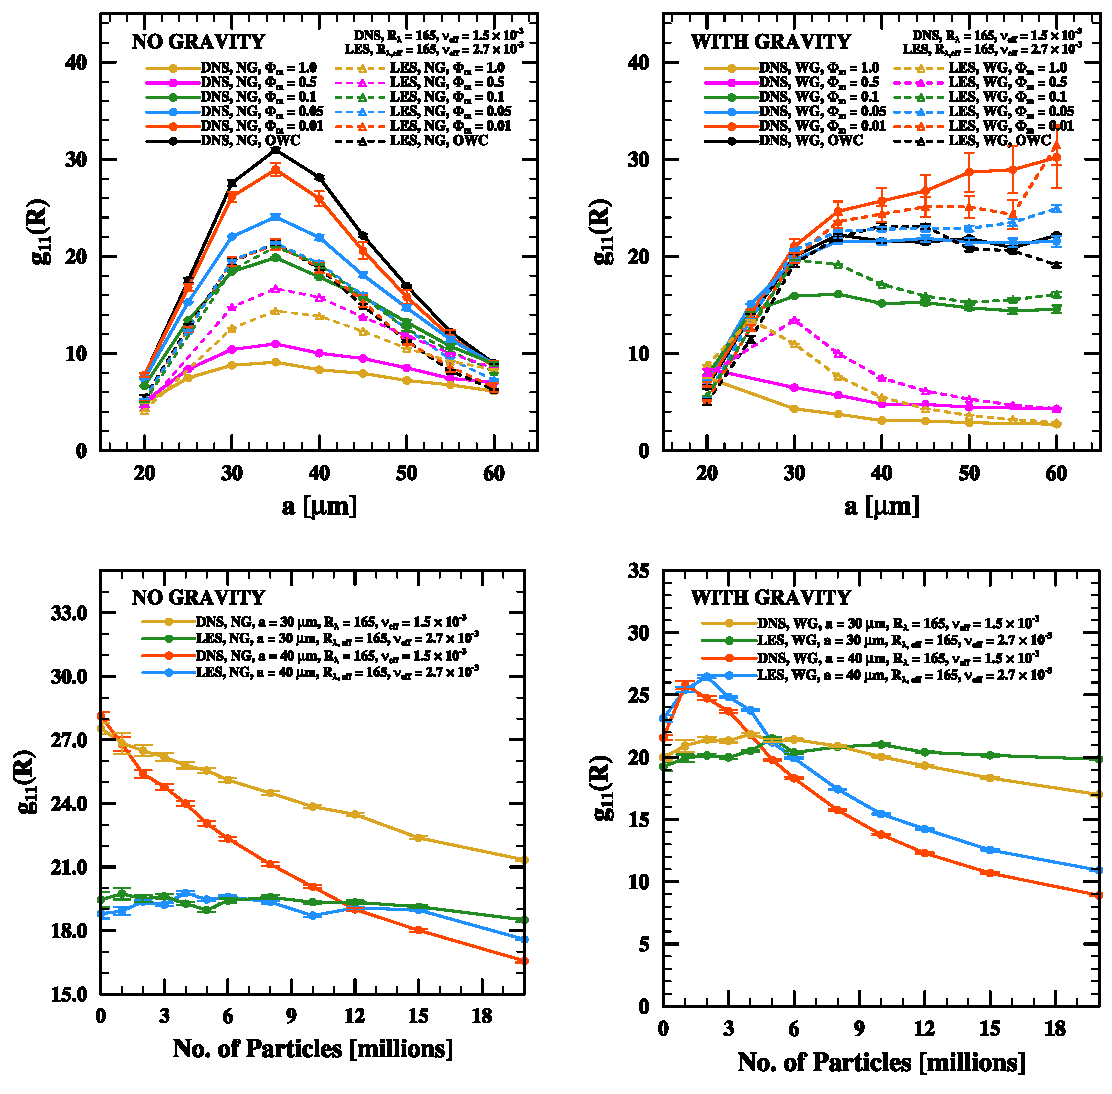
\includegraphics[width=13.5cm]{img/plots/2-2-3a-twcrdf.pdf}
\caption{
The values of radial distribution function (RDF) at contact distance for simulations with two-way momentum coupling using both DNS and LES.
Top plots show relation of RDF on particle radius for several fixed values of mass loading, $\Phi_m$ (also compared with results for OWC).
Bottom ones show relation of RDF on number of particles (in millions) for particles with radii $30$~$\upmu\text{m}$ and $40$~$\upmu\text{m}$.
Plots on the left show results without effects of gravity (NG), and those on the right consider settling particles (WG).
}
\label{fig:twcrdf}
\end{figure}


The results of LES for non-settling particles are consistent with those of DNS in terms of~general trends and significant reduction of the RDF as observed in simulations with OWC.
As observed in \textcite{Rosa2020} the RDF is barely sensitive to TWC and larger mass loadings (even as large as $\Phi_m = 1$, shown here) for both very small ($20$~$\upmu\text{m}$) and very large particles ($60$~$\upmu\text{m}$).
It is so, because small inertia particles have little impact on turbulence modulation and their behaviour in dominated by the fluid flow, while heavy particles are not very sensitive to influence of turbulence in general, and turbulence modulated by other particles in particular.
The same conclusion is valid for results from LES.
One interesting difference is the fact that results of LES are much less influenced by increasing mass loading.
For $\Phi_m \le 0.1$ mass loading seems to have very little effect on the RDF, and it can be seen for very large number of particles ($\Phi_m = 0.5, \, 1$), but still it remains larger that for DNS with corresponding mass loadings.
As shown before, see Section \ref{ssc:ch2.flow.twc}, large amount of heavy particles (when gravity is neglected) has tendency to weaken turbulence, which may result in reduced particle clustering.
In LES, smallest turbulent scales are parameterised by subgrid-scale model which is agnostic to any momentum transfer from particles to fluid, hence such dampening of smallest fluctuations cannot happen.
This may explain where, up to some point, LES is not sensitive to increasing mass loadings in TWC.
Still, large enough $\Phi_m$ are able to affect even larger turbulent scales that are directly resolved in LES, but this reduction is still not as dramatic as for DNS.

\begin{figure}[h]
\centering
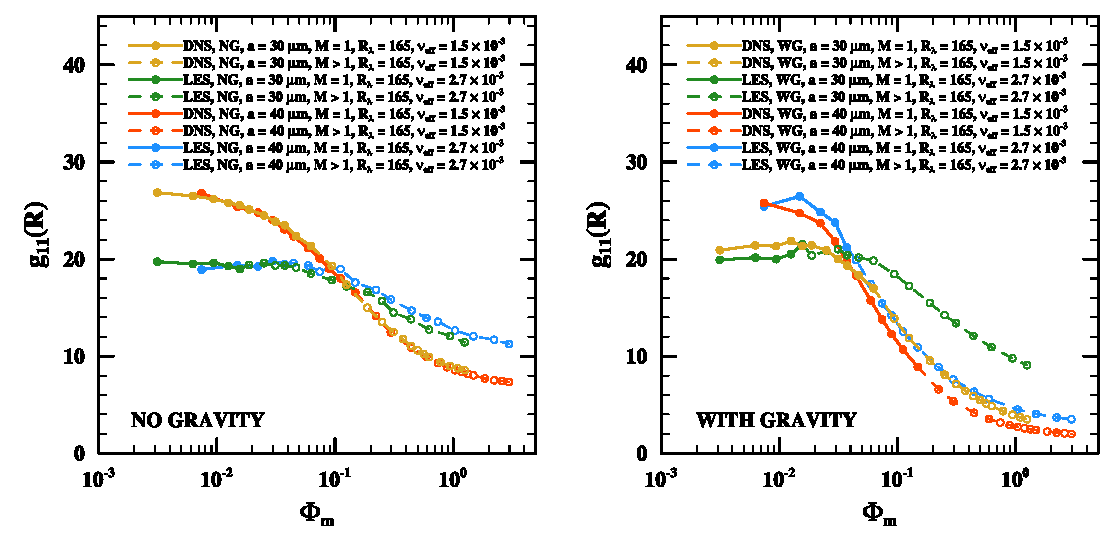
\includegraphics[width=13.5cm]{img/plots/2-2-3b-twcrdfext.pdf}
\caption{
Values of RDF for wider range of mass loadings.
It may be considered as extension of bottom plots from Figure \ref{fig:twcrdf}, where scope is limited to $20$ million particles, that give mass loadings of approximately $0.1$, depending on particle radii.
Here, results include range of mass loadings where TWC should be most prominent (i.e. around $0.1$ to $1$), and where may be insufficient (i.e. four-way coupling regime, for $\Phi_m > 1$).
Continuous lines represent simulations without superparticle parameterisation ($M=1$), while dashed ones show where it was necessary to obtain larger mass loadings.
For precise information of values of $M$ for each simulation, see Appendix \ref{app:spp}. 
}
\label{fig:twcrdfext}
\end{figure}


When settling particles are considered, results for LES do not follow those for DNS as closely as was in case of OWC simulations.
Still, results for LES follow similar pattern of initial ($a = 20$~$\upmu\text{m}$) strengthening of clustering (compared to OWC) then followed by gradual increase ending in plateau for heavier particles.
Moreover, we observe that for heavier particles ($60$~$\upmu\text{m}$) results of DNS and LES tend to converge.
Also, similarly to DNS, in TWC simulations with small mass loading ($\Phi_m \sim 0.01$), the RDF  in LES is also larger than obtained by OWC for the entire considered range of radii.

When we analyse the dependence of the RDF on the number of particles, we see clear differences between settling and non-settling particles.
When gravity is neglected, the RDF decreases monotonically with mass loading.
In simulations with gravity, however, initial increase and peak is observed, and then turns into monotonic decrease for larger mass loadings.
The prominence and position of such peak depends on the particle radius.

Interestingly, as in the case of OWC (see Figure \ref{fig:owcrdfrrv}), the results obtained by LES are much more aligned with DNS for settling particles.
When gravity is not considered, the RDF remains close to constant and almost completely insensitive to the increase in mass loading.
We have to look at larger picture (Figure \ref{fig:twcrdfext}) to notice that results from LES become sensitive to $\Phi_m$ at higher loadings ($\sim 0.3$), where they start to gradually decrease.
This is consistent with previous observations and its explanation.
When settling particles are considered, the results of LES seem to follow those from DNS more closely.
In general, there is small overestimation on part of LES, but for the most part it remains within acceptable range.
These discrepancies seem to be more significant for lighter particles, as they are more susceptible to TWC-agnostic turbulence from subgrid-scale model, as well as less capable of~turbulence modulation due to filtering of small-scale turbulence.
For heavier particles ($40$~$\upmu\text{m}$) these differences are smaller in absolute value and show consistent overprediction.
Moreover, based on data from Figure \ref{fig:twcrdf} (top right), it is expected that for larger particles results for DNS and LES should be more and more aligned.

As a side note, Figure \ref{fig:twcrdfext} is a great opportunity to showcase different regimes that depend on the amount of particles in the system.
Firstly, we have the \emph{one-way coupling regime}, which is approximately defined for mass loadings smaller than $0.1$, and where TWC is considered unnecessary to accurately model the system.
As pointed out by \textcite{Rosa2020}, even in this regime inclusion of TWC may provide physically significant adjustments.
This may be clearly seen in the plot, as the RDF is influenced by mass loading and starts decreasing much earlier than for $\Phi_m=0.1$.
Note, that this threshold is affected here by LES, due to filtering of small-scale structures, and effects of TWC start showing for $\Phi_m \sim 0.2$.
Then, for $0.1 < \Phi_m < 1$ we have \emph{two-way coupling regime}, where effects of TWC are most visible and necessary for physical fidelity.
This range of mass loadings is characterised by the steepest decrease in the RDF, as it is most sensitive to additional effects resolved due to two-way momentum coupling.
Finally, when $\Phi_m$ exceeds $1$ we say that such systems belong to the \emph{four-way coupling regime}, where TWC becomes insufficient and to provide its correct representation   it is necessary to~directly resolve interaction between particles.
It may be seen on the plot as the values of~RDF for this range of mass loadings start to plateau, signifying that TWC is not enough to entirely grasp complexity of system that is such densely packed with dispersed phase.

\medskip

\emph{The Radial Relative Velocity (RRV)}

Figures \ref{fig:twcrrv} and \ref{fig:twcrrvext} show radial relative velocities obtained from two-way coupled DNS and LES.
When DNS is considered, for smaller values of $\Phi_m$, not exceeding $0.1$, dependence of the RRV on particle sizes confirms results of \textcite[Fig. 22]{Rosa2020}.
For non-settling particles we observe only slight increase in the relative velocities with growing $\Phi_m$ for particles of intermediate radii ($30-50$~$\upmu\text{m}$).
This effect is direct consequence of two-way momentum coupling and is attributed to the transfer of momentum from particles to fluid that increases its local velocity, and, in turn affects neighbouring particles, further decorrelating their motion.
For settling particles, as expected, relatively large increase in the RRV is observed with growing particle inertia and mass loadings.
It is caused by strong modulation of turbulent flow by fast settling particles that create small-scale vortical structures with high angular momentum that highly impact relative motion of all particles.
The results for larger mass loadings not included in \textcite{Rosa2020}, i.e. $0.5$ and larger, are showing even stronger increase in the RRV for both settling and non-settling particles.
In Figure \ref{fig:twcrrv} (top right) lines for $\Phi_m=1$ were not included, as for $a = 60$~$\upmu\text{m}$ the RRV reaches normalised values of~$5.19 \, v_{k, \, \text{OWC}}$ for DNS and $4.86 \, v_{k, \, \text{OWC}}$ for LES.
This shows that effects described above are very strongly amplified as $\Phi_m$ rises.

\begin{figure}[h]
\centering
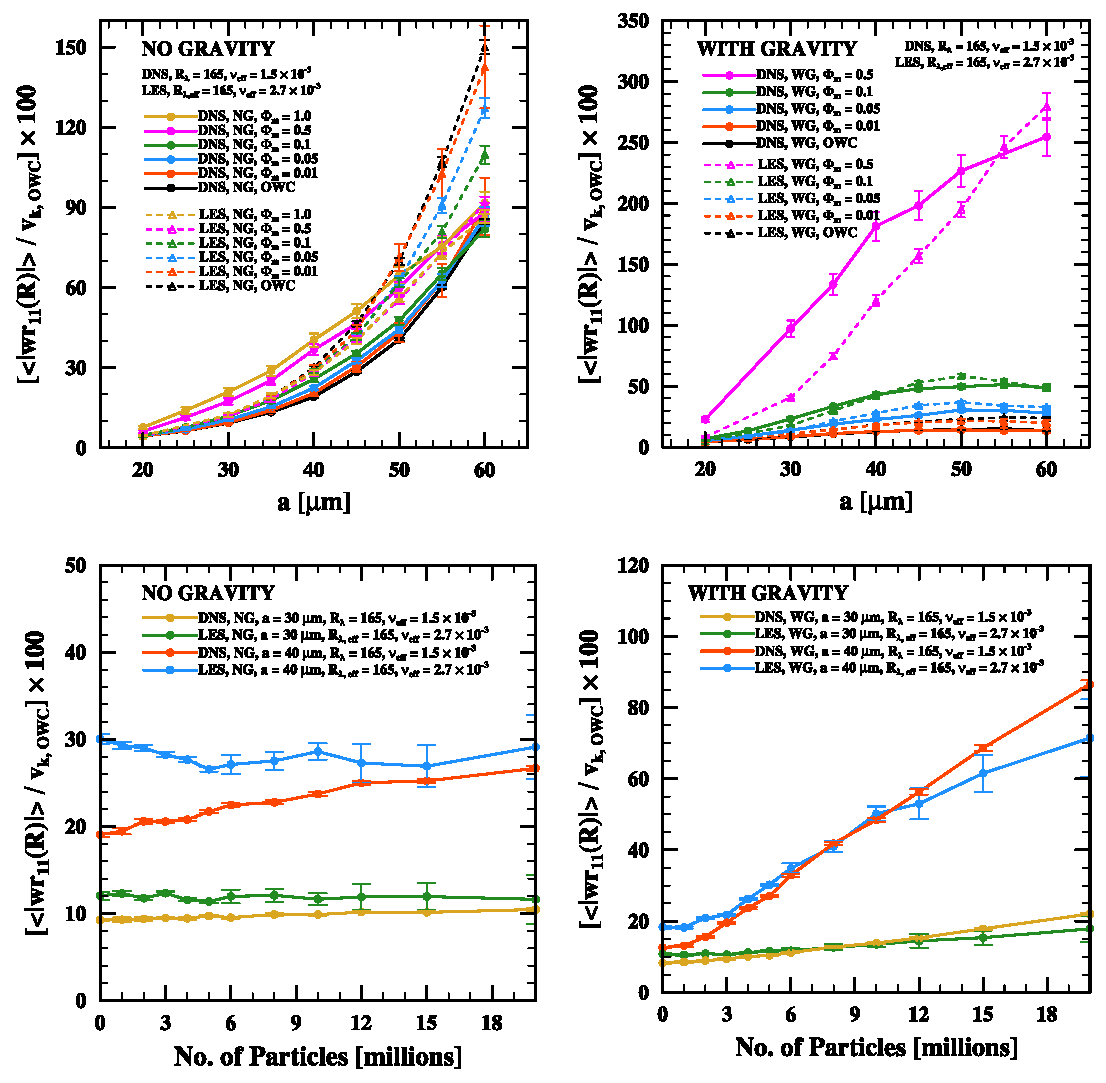
\includegraphics[width=13.5cm]{img/plots/2-2-3c-twcrrv.pdf}
\caption{
The values of radial relative velocity (RRV) at contact distance for simulations with two-way momentum coupling using both DNS and LES.
Consistent with Figure \ref{fig:twcrdf}.
}
\label{fig:twcrrv}
\end{figure}

The results of LES for non-settling particles show an important inversion of trend, as the effect of TWC (getting stronger with $\Phi_m$) is the relative decline in values of the RRV compared to OWC.
Also effects of TWC are still visible and getting more pronounced for high inertia particles ($60$~$\upmu\text{m}$), while in DNS particles of sizes around $55$~$\upmu\text{m}$ \parencite[Fig. 22a]{Rosa2020} are unaffected by TWC.
In Section \ref{ssc:ch2.coll.rdfrrv}, relatively high overestimation of the RRV in LES (OWC) was explained by filtering of small-scales of turbulence, thus eliminating decorrelating effects at these scales.
Inclusion of TWC cannot affect this directly, as subgrid-scale model is~agnostic to any momentum transfer from particles to fluid.
This influence of~TWC on~results for LES needs further investigation to explain this complex mechanism.

In case of particles affected by gravity the results are much more familiar (except already observed peculiar behaviour of the RRV for high mass loadings, $\Phi_m  \ge 0.5$).
We can observe that relative velocities from LES follow similar trend as for DNS.
Here, increase of the RRV is not only attributable to extra turbulent structures induced by fast settling particles but also to filtering of small-scale turbulence.
Thus, LES has tendency to overestimate DNS results, especially for heavy droplets ($40$~$\upmu\text{m}$ and larger).
With the increase of mass loading such overestimation becomes smaller, and for some range of smaller particles (depending on $\Phi_m$) the RRV in LES becomes underestimated.
This is because larger number of particles escalates turbulence modulation due to TWC effects which becomes dominant.
This influence, however, is stronger in DNS as also small scale turbulence is induced this way and not filtered as in LES.
For that reason such overestimation happens for lighter particles, as they are more susceptible to induced turbulence at smaller scales.

\begin{figure}[h]
\centering
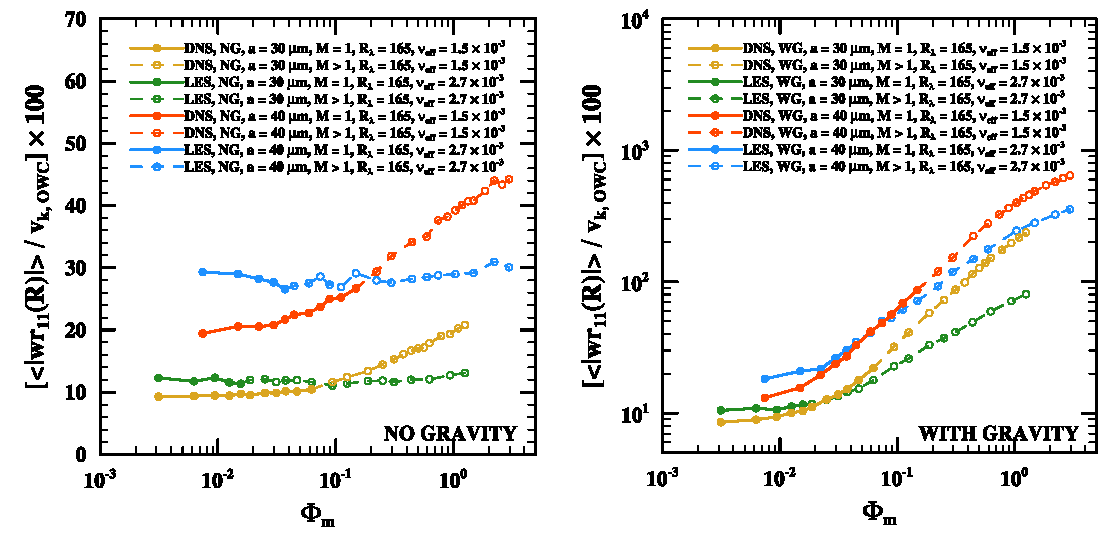
\includegraphics[width=13.5cm]{img/plots/2-2-3d-twcrrvext.pdf}
\caption{
Values of RRV for wider range of mass loadings.
Consistent with Figure \ref{fig:twcrdfext}.
}
\label{fig:twcrrvext}
\end{figure}

The effects of increasing mass loading on the RRV are opposite to those for the RDF, and relative velocities increase with larger numbers of particles in the system \parencite[Fig. 23 and 24]{Rosa2020}.
This increase is only slight or none without gravity, but for settling~particles it is much more dramatic, and explained by heavy turbulence modulation due to settling particles.
When LES is considered, we recognise similar pattern as in the case of RDF.
For non-settling particles and small enough mass loadings ($< 0.2$) the RRV is virtually constant and shows no signs of being affected by number of particles in the system.
Again, this is due to filtering of small-scale turbulence, limiting effects of turbulence modulation in TWC.
This effects become significant only for larger mass loadings, when intermediate scales can be affected due to larger concentration of particles.
In general, statistics obtained by LES quite closely follow those obtained by DNS, especially in the case of settling particles, and -- as with the RDF -- the quality of prediction improves for larger particles.  
 
\medskip

\emph{Collision Kernel}

Finally, we come to results concerning (dynamic) collision kernel (Figures \ref{fig:twcgamma} and \ref{fig:twcgammaext}).
In simulations without gravity, collision kernels show very little sensitivity to the effects of~TWC.
Still, we can observe slight decrease of $\Gamma^D_{11}$ with increasing mass loading.
This may be attributed to the fact that with growing number of particles the RDF is getting smaller, or -- equivalently -- distribution of particles in the system becomes more uniform.
Results obtained by LES are quite aligned with those from DNS, and similar trends are visible as for OWC (see Section \ref{ssc:ch2.coll.gamma}).
LES underestimates collision rate for smaller particles (up to $30$~$\upmu\text{m}$), but overestimates for those with larger radii.
The latter is mainly due to higher values of the RRV in LES, but with TWC this discrepancy is reduced as the overestimation of radial velocity by LES becomes smaller with increasing $\Phi_m$.
On the other hand, for larger mass loadings the RDF is much smaller in DNS than in LES, which makes drop in $\Gamma^D_{11}$ between OWC and high-$\Phi_m$ TWC larger.
Thus, for larger particles ($50-60$~$\upmu\text{m}$) the overprediction of~collision kernel by LES becomes larger.
Furthermore, since both the RDF and the RRV are unaffected by changes in mass loading until it reaches certain threshold ($\Phi_m \sim 0.2$, but should depend on particle size), the same is true for collision kernel.
Nonetheless, very crowded lines in Figure \ref{fig:twcgamma} (top left) are sign of very limited sensitivity of collision rate on effects of TWC and varying mass loading, as well as method used to obtain results (DNS or LES).
 
\begin{figure}[h]
\centering
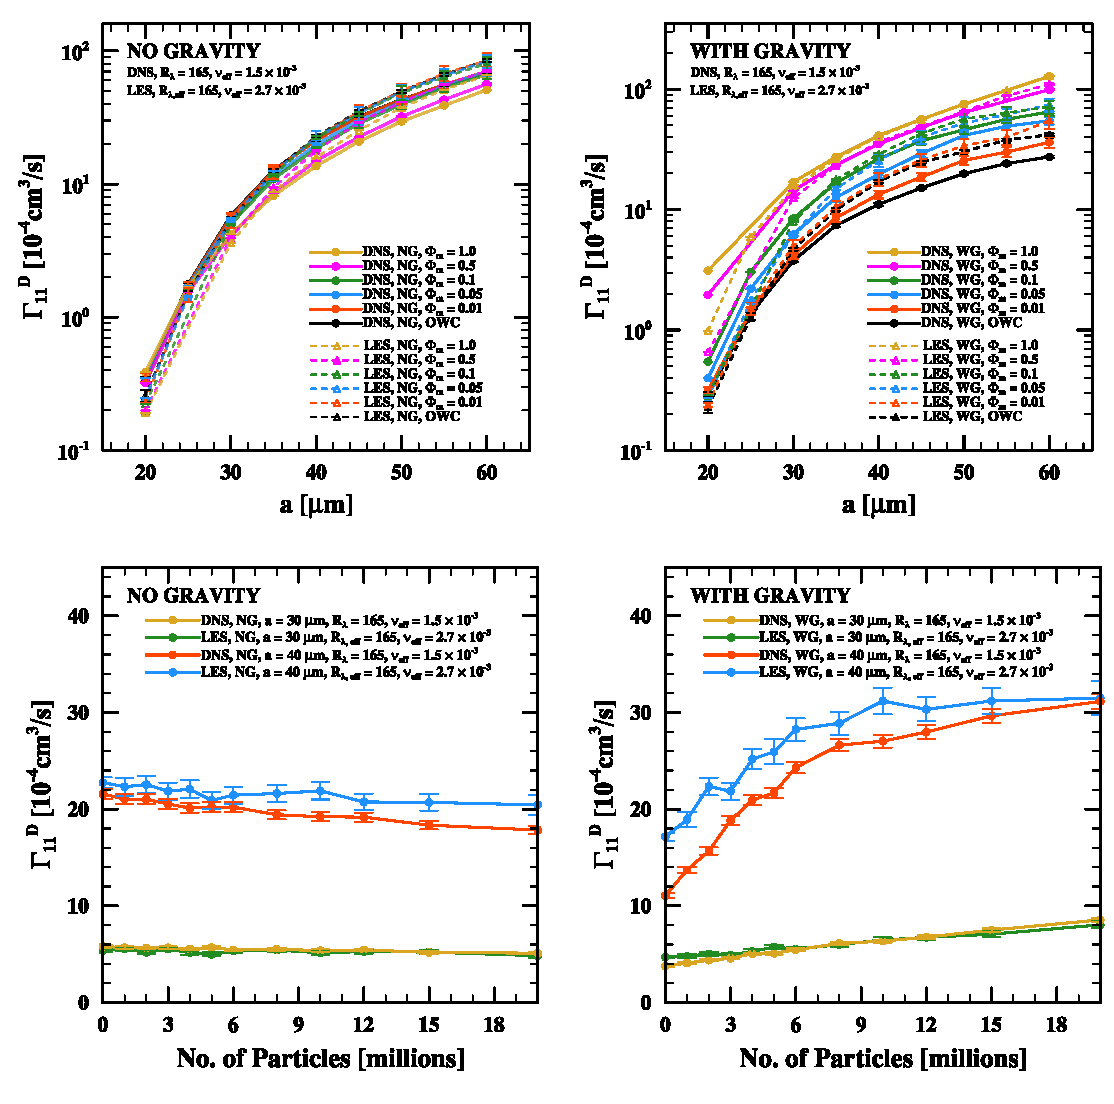
\includegraphics[width=13.5cm]{img/plots/2-2-3e-twcgamma.pdf}
\caption{
The values of dynamic collision kernel ($\Gamma_{11}^D$) for simulations with two-way momentum coupling using both DNS and LES.
Consistent with Figure \ref{fig:twcrdf}.
}
\label{fig:twcgamma}
\end{figure}

Results for settling particles show much more spread that indicates greater impact of TWC on collision rate in that case.
First of all, the general trend is opposite to that observed for particles unaffected by gravity.
The collision kernel is monotonically increasing with particle mass loading, due to stronger effects of turbulence modulation that lead to more clustering and higher relative velocities.
For LES, we observe similar phenomenon as for non-settling particles, where LES underpredicts collision kernel for smaller particles and overpredicts it for larger ones.
Also, as particles become heavier, the magnitude of such overshot decreases.
More importantly, we can observe that difference between DNS and LES becomes smaller and smaller as $\Phi_m$ increases.
In edge case, for $\Phi_m = 1$ and particles with radius $40$~$\upmu\text{m}$ or larger, results from DNS and LES are in perfect agreement.
On the flip side, the worst discrepancies between two methods also happen for large mass loadings ($\Phi_m \ge 0.5$), but for particles on the smaller side of the range considered (especially for $a = 20$~$\upmu\text{m}$).
This is effect of underprediction of the RRV by LES for simulations with large amounts of lighter particles, that are susceptible to small-scale turbulence induced in DNS that cannot be reproduced by~LES due to filtering of smallest scales of turbulence.

\begin{figure}[h]
\centering
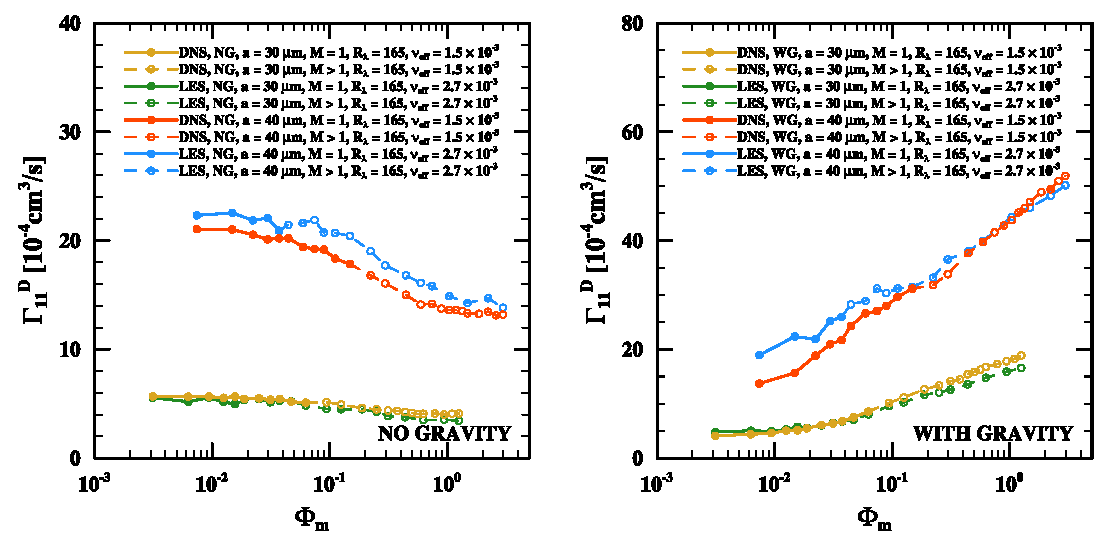
\includegraphics[width=13.5cm]{img/plots/2-2-3f-twcgammaext.pdf}
\caption{
Values of dynamic collision kernel for wider range of mass loadings.
Consistent with Figure \ref{fig:twcrdfext}.
}
\label{fig:twcgammaext}
\end{figure}

When we analyse dependence of $\Gamma^D_{11}$ on the amount of particles, again we can see that behaviour is different for non-settling and settling particles.
For the former, the collision kernel slightly decreases, while for the latter we can observe more definite increase in collision rate with increasing mass loading.
The collision kernel estimated by LES is in relatively good agreement with results obtained by DNS, and discrepancies seem to diminish with increasing mass loading of the dispersed phase.
What is interesting, even though kinematic statistics obtaied by DNS and LES were more aligned for particles of larger radius, $40$~$\upmu\text{m}$ in particular, for collision kernel we see the reverse.
Results for $a = 40$~$\upmu\text{m}$ are well aligned, in case of $a = 30$~$\upmu\text{m}$ we observe almost perfect agreement between two methods, both for small and large mass loadings.
This may be attributed to cancellations of certain effects specific to LES on kinematic statistics, that arise from filtering of small scales of turbulence, which cause underestimation of the RDF and overestimation of the RRV.





\chapter{Comparison of DNS and LES Performance}
\label{ch:ch3}

In this Chapter, the focus is on the issues of computational performance and comparison of DNS and LES on that field.
As introduced before, the main advantage of LES is its supposed edge in numerical efficiency, due to the reduction of grid size to which the turbulent flow is directly assigned.
This is the benefit that may outweigh, at least in some contexts, inaccuracies reported in Chapter \ref{ch:ch2} that are inherent to LES due to its parameterisation of small-scale turbulence.

In the following sections a more detailed analysis of the solver code is presented, especially in the context of its massively parallel execution.
Also, some previous results concerning its scaling with respect to the grid size and number of CPU cores used in execution shall be mentioned.
The core of following chapter, however, is the presentation of experimental measurements of code performance (in terms of wall clock time of its execution per time step) with respect to several parameters of interest.
In addition, more in-depth results, such as time spent on different stages of code, time used for communication between processes, and impact of the particle distribution on execution time, are analysed to validate and expand previous observations.


\section{Structure of Massively Parallel Simulation Code. Notes on Scaling}
\label{sc:ch3.perf}

First, we shall expand on Section \ref{sc:ch1.impl}, and provide more details on the architecture of the pseudo-spectral solver used in this study.
As stated before, it uses 2D decomposition to divide entire computational domain into column-like sections, or \emph{subdomains} (sometimes also referred to as ``pencils''), that are handled in parallel by individual processes with exclusively attributed blocks of memory.
This makes issue of communication and data transfer between subdomains critical in terms of performance.
For simulations used to obtain data in Chapter~\ref{ch:ch2}, as well as most data in this chapter (unless otherwise noted), most important execution parameters are gathered in Table \ref{tab:perfs-params}.

\begin{table}[h]
\centering
\scriptsize
\begin{tabular}{lrccrcrr}
 & $N$ & $N^3$ & Subdomain size & $\#\text{SD}$ & $N / \text{SD}$ & $N_{\text{proc}}$ & $\# \text{Nodes}$ \\ \hline
\textbf{DNS} & $256$ & $2^{24} \; (\sim 16.8 \, \text{M})$ & $16 \times 16 \times 256$ & $256$ & $2^{16}$ & $256$ & $11$ \\
\textbf{LES} & $64$ & $2^{18} \; (\sim 262 \, \text{k})$ & $8 \times 8 \times 64$ & $64$ & $2^{12}$ & $64$ & $3$ \\   
\end{tabular}
\caption{Standard execution parameters for DNS and LES code. $N$ - number of grid nodes in one direction; $N^3$ - total number of grid nodes; $\#\text{SD}$ - number of subdomains; $N / \text{SD}$ - number of grid nodes per subdomain; $N_{\text{proc}}$ - number of parallel processes used ($= \#\text{SD}$); $\# \text{Nodes}$ - number of \emph{Okeanos} supercomputer nodes (24 CPU cores per node) to fully saturate supported number of processes.
}
\label{tab:perfs-params}
\end{table}

It is notable that LES provides immense reduction on all axes of theoretical parameters that influence the complexity of fluid flow simulation.
Not only it requires resolution of fluid velocity field for $2^6 = 64$ times less nodes in total, but also every subdomain (handled by separate process) has $2^4 = 16$ times less nodes to compute.
Furthermore, the overall number of subdomains (and, equivalently, separate processes used) is smaller for LES by the factor of~$4$.
For supercomputer \emph{Okeanos} (ICM UW), where each computational node comprises of $24$ CPU cores, this leads to significant reduction of occupied computational nodes at one time from $11$ to $3$.

These parameters, however, are only related to the fluid flow computations and do not impact the effort that is necessary to resolve particles and particle-fluid interactions in the system.
This is especially vital in simulations with two-way momentum coupling, where particle-to-fluid ratio is of great importance, thus necessitating simulation of large numbers of computational particles to be tracked.
This issue has been already hinted at previously, as this is main reason for introduction of the super-particle parameterisation to achieve systems with considerably larger mass loadings.
Furthermore, it must be observed that codes used for DNS and LES are almost identical, barring additional LES code for computation of viscosity contribution from subgrid-scale model (see Table \ref{tab:code-steps}).
This has some clear advantages, as it provides better method comparability and code maintainability.
On the other hand, the parallel implementation of DNS is focused on splitting computations that become much less burdensome in LES as computations pertaining to particles tend to quickly dominate computational costs, as will be shown in the following sections.

\medskip

To achieve better understanding of the solver, Table \ref{tab:code-steps} provides the outline of the single time step being executed, divided into ten stages.
These stages are grouped into ones that are associated with \emph{fluid} (marked by ``F'' and greenish colours; Stages 1 and 7--10) and \emph{particles} (marked by ``P'' and brownish colours; Stages 2--6).
In addition, we distinguish stages that are not directly involved in simulation, but perform necessary post-processing of fluid and particle statistics (marked by ``d''; Stages 5 and 7).
Note, that fluid statistics are computed and stored only in certain intervals (here every $50$ steps when particles are involved, and every $10$ steps for particle-free simulations; in general, the frequency of data dumps can be adapted to the specific case).
Finally, there are Stages 3 and 9, that are enabled only for simulations with TWC or LES, respectively.

\begin{table}[!htbp]
\centering
\scriptsize
\begin{tabular}{p{10mm}p{75mm}p{25mm}p{27mm}}
\textbf{No.} \newline (Cat.) & \textbf{Name} \newline \emph{Description} & \textbf{Interdomain \newline communication} & \textbf{Notes} \\ \hline \hline
\rowcolor[RGB]{190,240,220} \textbf{1} \newline (F) & 
\textbf{Transform $\mathbf{\hat{u}}$ and $\boldsymbol{\hat{\omega}}$ to physical space} \newline \emph{Uses inverse 3D FFT twice; first two steps of pseudo-spectral method procedure.} & FFT & Eqn. \ref{eqn:psproc-1} and \ref{eqn:psproc-2}. \\ 
\rowcolor[RGB]{240,220,190} \textbf{2} \newline (P) & 
\textbf{Calc. momentum transfer from fluid to particles} \newline \emph{Finds closest grid points to particles, and calculates momentum transfer using six-point Lagrange interpolation scheme (OWC).} & Local & --- \\ 
\rowcolor[RGB]{240,190,150} \textbf{3} \newline (P) &
\textbf{Calc. momentum transfer from particles to fluid} \newline \emph{Uses PNN kernel to apply momentum transfer projected from particles onto fluid at neighbouring grid points (TWC).} & Local & Eqn. \ref{eqn:twc-px}. \newline \textbf{(TWC only)} \\ 
\rowcolor[RGB]{240,220,190} \textbf{4} \newline (P) &
\textbf{Calc. new particle velocities and positions} \newline \emph{Integrate equations of motion for particles to obtain their new velocities and positions; update data structures used to keep track of neighbouring particles.} & Local & Eqn. \ref{eqn:owc}. \\ 
\rowcolor[RGB]{240,240,170} \textbf{5} \newline (Pd) &
\textbf{Calculate and write particle collision statistics} \newline \emph{Detection a counting of particle collision ($\Gamma^D_{11}$) and relative particle pair data within radial shells necessary to~compute RDF and RRV.}  & Global (only to \newline write data), Local & Sec. \ref{ssc:ch2.coll.rdfrrv} and \ref{ssc:ch2.coll.gamma}; \newline every step;  for steps \newline $> 30 000$ (after \newline system relaxation). \\ 
\rowcolor[RGB]{240,220,190} \textbf{6} \newline (P) &
\textbf{Update particle velocities and positions} \newline \emph{Change the state of particles as calculated in step 4; transfer data for particles crossing subdomain boundaries.} & Global, Local & --- \\ 
\rowcolor[RGB]{150,240,150} \textbf{7} \newline (Fd) &
\textbf{Calculate and write flow statistics and spectra} \newline \emph{Energy and dissipation spectra are obtained and stored; other base flow statistics ($u'$ and $\epsilon$) and derived statistics are calculated.} & Global, FFT, Local & Sec. \ref{ssc:ch2.flow.bstat} and \ref{ssc:ch2.flow.spec}; \newline every 50 steps*. \\ 
\rowcolor[RGB]{190,240,220} \textbf{8} \newline (F) & 
\textbf{Transform $\mathbf{u} \times \boldsymbol{\omega}$ to spectral space} \newline \emph{Uses 3D FFT to perform third step of pseudo-spectral method procedure; performs post-transform dealiasing.} & FFT & Eqn. \ref{eqn:psproc-3}. \\
\rowcolor[RGB]{150,190,240} \textbf{9} \newline (F) & 
\textbf{Calc. effective viscosity using subgrid-scale model} \newline \emph{Uses fluid energy spectrum and subgrid-scale model formulation to adjust kinematic viscosity with spectral-eddy viscosity, i.e. $\nu + \nu_e(k|k_c)$.} & Global & Eqn. \ref{eqn:sgs-1} and \ref{eqn:sgs-2}. \newline \textbf{(LES only)} \\ 
\rowcolor[RGB]{190,240,220} \textbf{10} \newline (F) &
\textbf{Integrate fluid flow equations} \newline \emph{Fourth step of pseudo-spectral method; integrates 3D Navier-Stokes equation using Crank-Nicholson scheme; incorporates deterministic forcing and other external forces; performs necessary dealiasing and symmetrisation.} & Global, Local & Eqn. \ref{eqn:psproc-4} \\ \hline \hline
\end{tabular}
\caption{
The outline of a single time step of the pseudo-spectral solver used in this study divided into ten stages.
Labels in the first column indicate whether given stage is related to solving fluid flow (''F'') or particles (''P''), and whether it is concerned with gathering and postprocessing data (''d'').
The~third column characterises the level of interdomain communication required at given stage. \newline
* -- for simulations without particles flow statistics are gathered more frequently (here, every 20 steps).
}
\label{tab:code-steps}
\end{table}

The second column of Table \ref{tab:code-steps} provides general name and overview of computations performed at given stage.
For more information on general procedure of pseudo-spectral method, see Appendix \ref{app:psm}.
The outline of strategy used to calculate particle-pair statistics (Stage 5) was described in Sections \ref{ssc:ch2.coll.rdfrrv} and \ref{ssc:ch2.coll.gamma}.
More information on detailed implementation, involving linked lists and call-index method may be found in \textcite{Allen1987} and \textcite{Onishi2013}.
As for LES- and TWC-specific stages, these computations are outlined in Sections \ref{sc:ch1.les} and \ref{sc:ch1.part}, respectively.
See ''Notes'' column for additional references.

\begin{figure}[h]
\centering
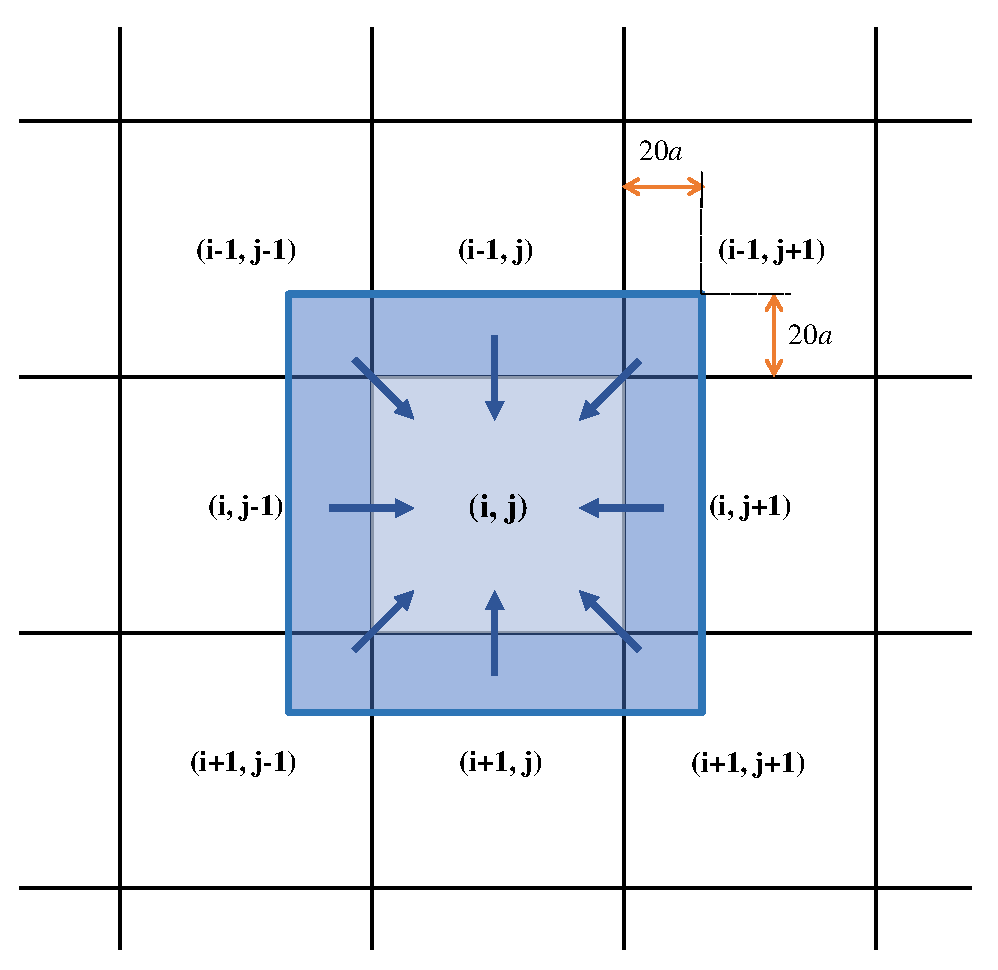
\includegraphics[width=9cm]{img/figs/halo.pdf}
\caption{
The halo region of a host process that overlaps with eight neighbouring subdomains in~2D~decomposition.
The range of overlap is $10R = 20a$, which is the largest possible outer radius of~spherical shells used to calculate kinematic statistics of particles for particle located at the subdomain boundary.
Arrows indicate the direction of data transfer.
Illustration based on Figure 3 in \textcite{Ayala2014}. 
}
\label{fig:halo}
\end{figure}

Finally, Table \ref{tab:code-steps} contains distilled information on the severity of communication between processes required in given stage.
Stages marked with ``Local'' involve only communication between eight neighbouring subdomains in the physical space.
This communication is for the most part due to necessary exchange of fluid velocity field data for grid nodes on the subdomain boundary, or transfer of particle data when they pass through such boundaries, as in Stage 6.
This communication is performed using MPI functions: \texttt{MPI\_SEND}, \texttt{MPI\_RECV}, and \texttt{MPI\_SENDRECV}.
This is also an important part of the data exchange when postprocessing particle data within Stage 5, as counting of kinematic statistics involves detection of particle pairs in spherical shells of radii related to particle radii.
These shells may overlap subdomain boundaries, hence it is necessary to transfer states of particles from regions of surrounding subdomains that may be affected \parencite{Ayala2014}.
These extra regions are referred to~as~the~\emph{halo regions}.
For illustration, see Figure \ref{fig:halo}.

The label ``Global'' refers to data exchange between multiple, and often all, processes and requires large degree of synchronisation between processes.
It is associated with MPI functions: \texttt{MPI\_BCAST}, \texttt{MPI\_REDUCE}, and \texttt{MPI\_ALLREDUCE}.
It is often involved in stages used in computation of statistics.
The postprocessing of turbulence statistics (Stage 7) requires global data of the entire fluid velocity field.
On the other hand, gathering of particle-pair statistics (Stage 5) is mostly local, requiring only information on neighbouring particles in halo regions.
The only global aspect of its interprocess communication comes into play at the end, when all data is transferred to the one process that is responsible for disk I/O~operations.
The~\texttt{MPI\_ALLREDUCE} calls in Stages 9 and 10 cover necessary summations over fluid energy spectrum in the Fourier space.
In the former case, it is necessary to calculate and~redistribute to all processes the spectral-eddy viscosity in LES.
For the last stage, such global synchronisation is necessary due to application of large-scale forcing, which is implemented in a sequential manner.
Also, to a limited degree, the data reduction along single axis is necessary in the symmetrisation of fluid velocity after Fourier transform \parencite{Ayala2014}. 
Thus, we may observe that such synchronisation in LES-specific code should not negatively impact entire execution flow, as another global communication is imposed soon after for DNS as well. 

The very particular category of communication involves performing 3D fast Fourier transforms over the entire domain, as part of the pseudo-spectral solver in Stages 1 and 8 (also, less frequently, when gathering flow statistics).
It is marked by ``FFT''.
As previously mentioned, this code utilises effective implementation of 3D FFT for distributed domains introduced in~\textcite{Dmitruk2001}, adjusted for 2D domain decomposition \parencite{Ayala2013}.
It uses strategy known as the \emph{transpose method} that exploits the fact that multidimensional FFT may be decomposed into sequence of nested 1D FFTs.
Three consecutive 1D FFTs are performed in the direction of subdomain columns, or ''pencils'', where domain is not subdivided, to avoid interprocess communication during computation of the transform.
Of course, to obtain result equivalent to 3D FFT, it is necessary to transpose entire domain between and after 1D FFT calls, so they are effectively computed along all three axes.
This approach has been shown to be scalable with number of CPU cores used \parencite{Dmitruk2001,Ayala2013}.
Still, this transposition incurs relatively high cost due to necessary data transfer involving all processes.

\smallskip

Note, that this study focuses on single grid size for DNS and LES.
Thus, we are not equipped with data suitable for a broader analysis of code scalability with respect to $N$, as~well~as the~number of~CPU cores used, $N_{\text{proc}}$, in a systematic manner.
Some analyses of code performance when number of CPU cores available is limited, i.e. when execution is starved for resources, is presented in the following section, but it cannot be taken as a~replacement for proper scalability study.
Fortunately, this implementation of the pseudo-spectral method has already been thoroughly studied in this respect.
The study by \textcite{Ayala2014} stands out with in-depth analysis of scaling for simulations without TWC (but with modelling of~hydrodynamic interactions between particles), as well as development of interesting tools and concepts for more analytical, hardware-independent investigation of the code scalability. 

This thesis is more focused the impact of simulating particles on the overall performance.
This is crucial, since it appears to be the dominating factor for LES.
Moreover, the influence of TWC on computational complexity was not thoroughly surveyed yet.
\textcite[Fig. 1]{Rosa2022} shows simple scalability study of TWC simulations with respect to~particle~radius and mass loading, to show difficulty of effectively attaining high $\Phi_m$ in simulations with smaller particles.
Thus, some broader analysis on these subjects is presented in the following sections.



\section{Results of Basic Performance Measurements}
\label{sc:ch3.perfs}

To analyse impact of particles on the performance in the pseudo-spectral code, the time of~execution (so-called \emph{wallclock time}, WCT) of individual steps were measured.
These measurements were taken for a single process, as global data transfer between processes at the end of each time step (Stage 10) has synchronising effect on all processes, so impact of such simplification is minimal.
For the remainder of this chapter these timings, averaged over the entire run of simulation, shall be denoted by $T$.
All uncertainties listed and marked on plots in this and following sections are standard deviations of these measurements.
Such deviations are relatively large, but this is expected, as measurements involve a certain degree ``natural'' variability between time steps, e.g. longer processing times  whenever flow statistics are computed (i.e. every 10 or 50 time steps).
In addition, when comparison between DNS and LES is~of~interest, we present results in abstract unit of workload, $(T \times N_{\text{proc}})$, obtained by multiplying average WCT per step by the number of CPU cores used at the same time in the parallel execution (expressed in ``CPU-seconds'').
This measurement may serve as~an~approximation of the average amount of work, or used computational resources, per time step.

\begin{figure}[h]
\centering
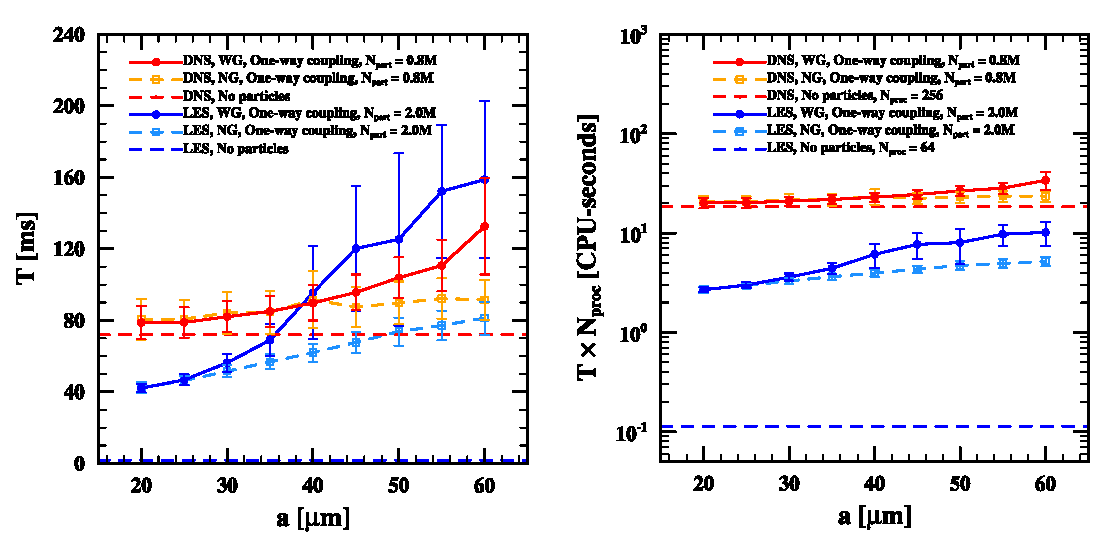
\includegraphics[width=13.5cm]{img/plots/3-2a-pfsowc.pdf}
\caption{
Time-averaged wallclock times per step by itself (left) and multiplied by number of~parallel processes used to execute code (right, in log scale) for simulations under one-way momentum coupling (OWC), depending on particle radii. Both results for DNS and LES are presented, with and without gravity (WG and NG, respectively). Horizontal dashed lines represent values for simulations without particles.
}
\label{fig:pfsowc}
\end{figure}

Figure \ref{fig:pfsowc} shows the dependence of execution time on particle radius for simulations under one-way momentum coupling, as well as without particles.
We observe that WCT per time step increases monotonically with particle radius, both in DNS and LES, when gravity is considered and without it.
Moreover, in case of simulations with settling particles, the~impact of larger droplet radii is much stronger.
In part, these results may be explained by the fact that size of the halo region used to compute two-point particle statistics becomes larger with particle radii.
This means that more data related to the state of neighbouring particles needs to be transferred to the host process.
This implementation detail may explain slight increase in computational cost, as in case of results without gravity, but hardly such increase as is observed when gravity is considered.
More importantly, the clear difference between performance of simulations with and without gravity, predominantly for high inertia droplets ($a > 40$~$\upmu\text{m}$), cannot be explained in simple terms, as enabling gravity in the solver code should have no direct bearing on its computational complexity.
This effect shall be further examined in following sections.

Note, that some attention was given to the effects of droplet radii on simulation performance, but other aspects have been emphasised.
In \textcite[Fig. 8c]{Ayala2014} the theoretical scaling analysis of Hybrid DNS code with respect to the sizes of droplets was conducted.
The~comparison was made between simulations where liquid water content (LWC) was held constant, which is comparable to $\Phi_m$ in this study.
Thus, simulations with smaller droplets required more individual particles to be tracked, increasing execution time.
It should be mentioned that simulations in \parencite{Ayala2014} were carried out under OWC, but with consideration of aerodynamic interactions between droplets. 
Similar results were shown in \textcite[Fig. 1b]{Rosa2022}, with respect to TWC.
More interestingly, in the same paper (see Fig. 1a therein) it was argued that when the same number of particles is used, the execution time is broadly independent of particle radii.
These results, however, were performed only for non-settling particles.

Furthermore, the comparison of results obtained for DNS and LES confirms expectations that were previously anticipated.
Firstly, when only particle-free fluid simulation is concerned, LES is much faster due to reduced grid size.
This is even more pronounced for~$(T \times N_{\text{proc}})$, where LES consumes two orders of magnitude less resources.
On the other hand, results for~LES exhibit much larger difference in execution times between flow-only simulations and~those with particles.
For DNS the extra computational cost of simulating 2 million particles (on average $\sim 7.8\text{k}$ per subdomain) is barely noticeable, while for LES processing of~800k particles ($12.5\text{k}$ per CPU core) seems to be dominating the execution time. 

\begin{figure}[h]
\centering
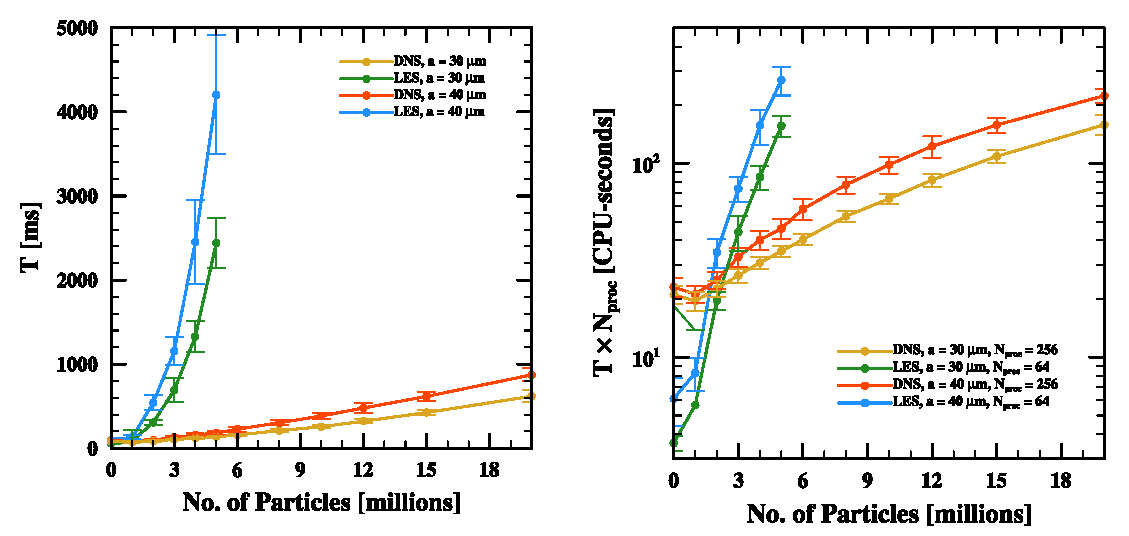
\includegraphics[width=13.5cm]{img/plots/3-2b-pfstwc.pdf}
\caption{
Time-averaged wallclock times per step by itself (left) and multiplied by number of~parallel processes used to execute code (right, in log scale) for simulations under two-way momentum coupling (TWC, with gravity), depending on number of computational particles. Both results for~DNS and LES are presented.
}
\label{fig:pfstwc}
\end{figure}

The above observation is thoroughly confirmed by similar measurements made for simulations under two-way momentum coupling with varying number of particles (considering gravity).
These results are shown in Figure \ref{fig:pfstwc}.
When the number of particles is increased, execution times per step quickly become prohibitively large.
That is the reason behind very limited range (up to 5 million) of particle counts in LES simulations, and any larger mass loadings had to be achieved via superparticle parameterisation.
This is in stark contrast with DNS, where simulations with 20 million computational particles could be easily performed.
For illustration, on the hardware used to run these simulations (\emph{Okeanos}), the total running time of LES with more than 5 million particles would easily exceed 2 days (i.e. maximal time of a single job), while DNS with 20 million particles (largest used) would be able to compute almost $2.5$ times more time steps in the same amount of wallclock time.
Longer simulation times are beneficial, as they result in lower statistical uncertainty of the modelled parameters.

This result, even though expected, is much more severe than anticipated, and -- given this code and parallelisation architecture -- makes LES completely untenable for TWC simulations with even moderate mass loading.
One simple remedy for this issue is the use of super-particle model, as in this study, but it combines two types of parameterisations, i.e.~superparticles and subgrid-scale model, whose interaction is not well known, thus rendering veracity of~such~results fragile at best.
In the long run, the best solution would be establishing the parallelisation strategy for LES that relies not only on decomposition of grid used to compute fluid flow (as~with~current implementation, tailored for DNS) but also for particles, which clearly are the bottleneck.

On another note, results shown in Figure \ref{fig:pfstwc} corroborate claims of \textcite{Rosa2022} that scaling of TWC DNS with respect to the number of particles is close to linear.
Furthermore, the measurements for TWC (both DNS and LES) confirm that the computational effort increases with growing particle sizes.

\medskip

It was already mentioned that since this study is confined to one specified grid size, $N$, proper scaling analysis in relation to $N$ and $N_\text{proc}$ is not feasible.
Instead, figure \ref{fig:pfspfn} shows wallclock times for a range of DNS simulations in relation to maximal number of computational nodes on supercomputer \emph{Okeanos} (24 CPU cores per node) that were set as a~hard limit for the running code to utilise.
It is important to point out that these simulations still exhibit standard grid size and division into subdomains (see Table \ref{tab:perfs-params}).
Thus, optimal number of~parallel processes executing the code remained unchanged.
These results, therefore, provide information on the performance of simulations when it is starved for resources, i.e.~the ratio of executing processes and available CPU cores is more than $1$.

\begin{figure}[h]
\centering
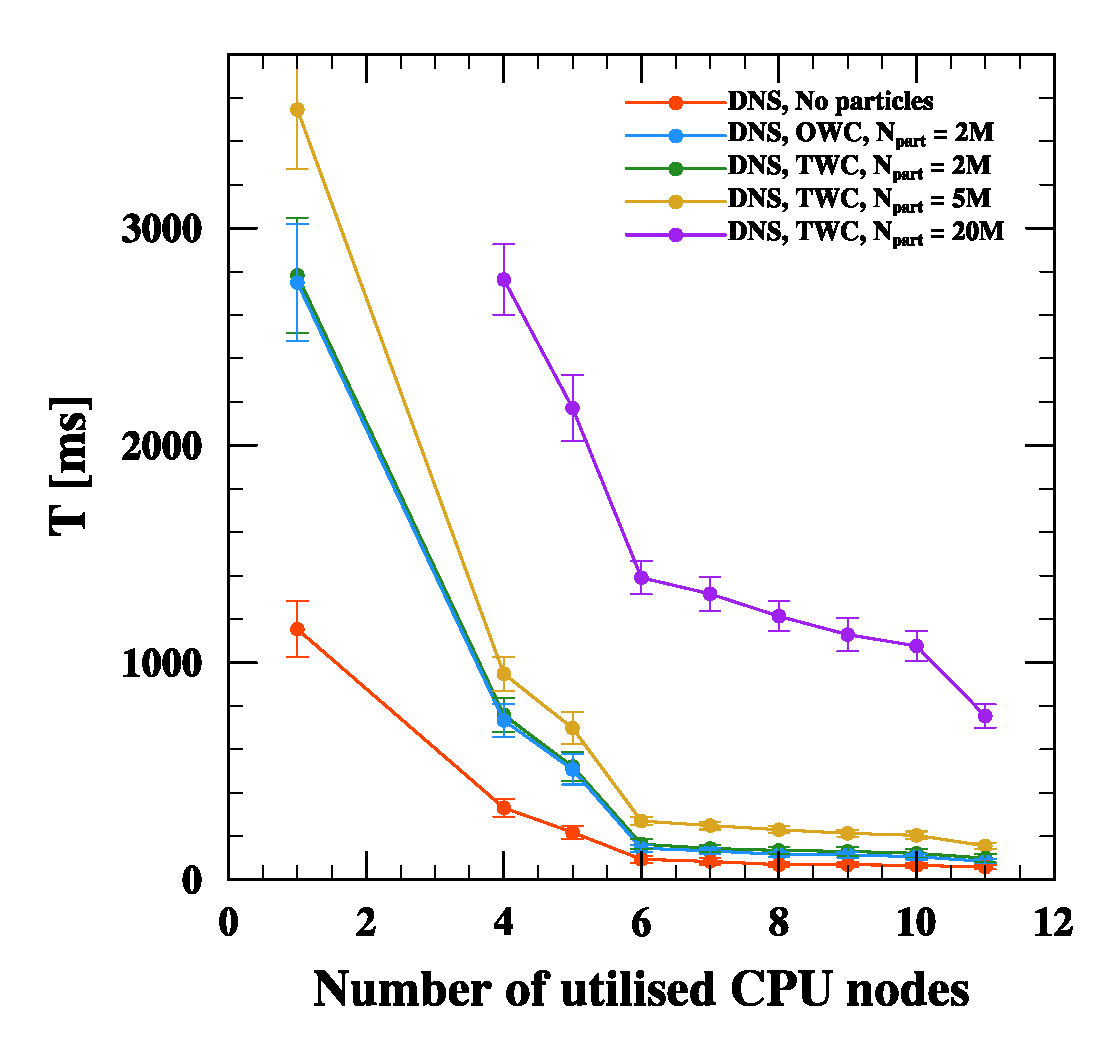
\includegraphics[width=8cm]{img/plots/3-2d-pfspfn.pdf}
\caption{
Time-averaged wallclock times per step for DNS, depending on limited number of~computational nodes on \emph{Okeanos} supercomputer (24 CPU cores per node).
DNS code supports up to $256$ parallel processes in execution, hence value of $11$ represents optimal saturation of processes with available CPU cores.
}
\label{fig:pfspfn}
\end{figure}

The number of nodes enough to saturate all processes for ``standard'' DNS is $11$ (see Table~\ref{tab:perfs-params}).
When the number of available nodes is limited, we observe interesting behaviour where execution time increases linearly within certain intervals that are separated by radical drops in the computational performance.
These drops, somewhat expectedly, coincide with thresholds where the ratio of the number of processes, $N_{\text{proc}}$, to the number of available CPU cores, $N_{\text{CPU}} = 24 \times \#\text{Nodes}$, becomes larger than consequent whole numbers.
For example, for $6$ Nodes such ratio is approximately $1.78$, which indicates that, in simple terms, each CPU core serves one process, and than another, with some CPU cores to spare.
For $5$ Nodes, however, $N_{\text{proc}} / N_{\text{CPU}} \approx 2.13$, thus every CPU has to serve two processes, and then there are still some remaining to be executed.
This code, as outlined in Table \ref{tab:code-steps}, requires significant degree of local and global synchronisation between processes, hence such remaining processes, even if few, put free CPU cores on hold waiting for all processes to complete. 
In addition, certain time overhead must be accounted for queuing software and operational systems of~nodes to handle more frequent preemptions and context switches between processes.

\begin{table}[h]
\centering
\scriptsize
\begin{tabular}{lrrrr}
\textbf{LES} & \multicolumn{4}{c}{Wallclock time per step [ms]} \\
& No particles & OWC, $N_{\text{part}} = 2 \text{M}$ & TWC, $N_{\text{part}} = 2 \text{M}$ & TWC, $N_{\text{part}} = 5 \text{M}$ \\ \hline
1 node utilised             & $112.90 \pm 22.71$ & $1250.07 \pm 81.70$ & $1281.39 \pm 80.65$ & $6407.73 \pm 303.50$ \\
2 node utilised             & $2.22 \pm 0.33$ & $462.62 \pm 30.51$ & $488.70 \pm 35.98$ & $3348.79 \pm 118.54$ \\
3 node utilised (saturated) & $1.77 \pm 0.34$ & $249.76 \pm 17.41$ & $260.68 \pm 19.34$ & $1914.37 \pm 90.85$ \\
\end{tabular}
\caption{Time-averaged wallclock times per step for LES, depending on limited number of computational nodes on \emph{Okeanos} supercomputer (24 CPU cores per node).
Consistent with Figure \ref{fig:pfspfn}.
}
\label{tab:perfs-pfnles}
\end{table}

For completeness, results of similar measurements for LES are shown in Table \ref{tab:perfs-pfnles}.
These results show similar pattern, although it is harder to discern due to limited range of nodes that can be utilised due to limited number of subdomains.
The only outlier is the exorbitantly high value for simulation without particles when limited to only single node.
This, however, may be at least in part explained by aforementioned overhead due to process switching that seems to dominate otherwise very fast flow-only computations with LES.

In addition, both OWC and TWC simulations with the same number of particles (2~million) are considered.
These results clearly show that additional computations due to TWC (Stage 3) have barely noticeable influence on the execution times.
Thus, it is not TWC itself that makes simulations slower, but the necessity of increasing the number of particles in the system to obtain physically significant results.

\begin{table}[h]
\centering
\scriptsize
\begin{tabular}{lrrrrrr}
\multicolumn{7}{c}{\textbf{Wallclock time per step [ms]}} \\
 & & No particles & OWC & TWC & TWC & TWC \\ 
Subdomain size & $N / \text{SD}$ &  & $N_{\text{part}} = 2 \text{M}$ & $N_{\text{part}} = 2 \text{M}$ & $N_{\text{part}} = 5 \text{M}$ & $N_{\text{part}} = 20 \text{M}$ \\ \hline

DNS, $8 \times 8$ & $2^{14}$ & $24.6 \pm 7.4$ & $39.2 \pm 8.1$ & $41.9 \pm 7.7$ & $60.0 \pm 11.0$ & $2015.2 \pm 29.4$ \\
\textbf{DNS}, $\mathbf{16 \times 16}$ & $2^{16}$ & $58.3 \pm 10.2$ & $89.7 \pm 9.8$ & $97.6 \pm 9.4$ & $180.0 \pm 20.8$ & $872.5 \pm 76.2$ \\
DNS, $32 \times 32$ & $2^{18}$ & $192.0 \pm 43.2$ & $310.6 \pm 45.0$ & $317.8 \pm 44.0$ & $551.8 \pm 45.9$ & $3046.2 \pm 139.4$ \\ \hline
\textbf{LES}, $\mathbf{8 \times 8}$ & $2^{12}$ & $1.8 \pm 0.3$ & --- & $338.4 \pm 29.5$ & $2539.7 \pm 246.5$ & --- \\
LES, $16 \times 16$ & $2^{14}$ & $4.1 \pm 0.5$ & $1359.4 \pm 49.1$ & $1425.9 \pm 52.4$ & $9142.4 \pm 290.8$ & --- \\ \hline \hline
 & & & & & & \\
\multicolumn{7}{c}{$\mathbf{(}$\textbf{WCT [s]} $\mathbf{\times N_{\text{proc}})}$ \textbf{per step}} \\
 & & No particles & OWC & TWC & TWC & TWC \\ 
Subdomain size & $N_{\text{proc}}$ &  & $N_{\text{part}} = 2 \text{M}$ & $N_{\text{part}} = 2 \text{M}$ & $N_{\text{part}} = 5 \text{M}$ & $N_{\text{part}} = 20 \text{M}$ \\ \hline

DNS, $8 \times 8$ & 1024 & $25.2 \pm 7.5$ & $40.01 \pm 8.2$ & $42.9 \pm 7.8$ & $61.4 \pm 11.3$ & $220.4 \pm 30.1$ \\
\textbf{DNS}, $\mathbf{16 \times 16}$ & 256 & $14.9 \pm 2.6$ & $23.0 \pm 2.5$ & $25.0 \pm 2.4$ & $46.1 \pm 5.3$ & $223.4 \pm 19.5$ \\
DNS, $32 \times 32$ & 64 & $12.3 \pm 2.8$ & $19.9 \pm 2.9$ & $20.3 \pm 2.8$ & $35.3 \pm 2.9$ & $195.0 \pm 8.9$ \\ \hline
\textbf{LES}, $\mathbf{8 \times 8}$ & 64 & $0.113 \pm 0.022$ & --- & $21.7 \pm 1.9$ & $162.5 \pm 246.5$ & --- \\
LES, $16 \times 16$ & 16 & $0.066 \pm 0.008$ & $21.8 \pm 0.8$ & $22.8 \pm 0.8$ & $146.3 \pm 4.7$ & --- \\ \hline \hline
\end{tabular}
\caption{Time-averaged wallclock times per step by itself (top) and multiplied by the number of~parallel processes used to execute code (bottom) for DNS and LES simulations with different sizes of computational subdomains.
Entries in bold represent ``standard'' (see Table \ref{tab:perfs-params}) sizes used in this study.
}
\label{tab:perfs-pfg}
\end{table}

For another, slightly different set of the performance data, see Table \ref{tab:perfs-pfg}.
It shows how $T$ and $(T \times$ $N_{\text{proc}})$ are affected by changes in sizes of computational subdomains.
Rows marked in bold represent standard sizes used throughout this study (see Table \ref{tab:perfs-params}).
These results, limited they are, show some aspects of code scaling and certain tradeoff that has to be taken into account when choosing appropriate level of domain subdivision.

This is quite well exemplified by the results for DNS.
On one hand, obviously, the execution time per iteration (and, thus, total time taken by simulation) decreases when such subdivision becomes finer, as the number of grid nodes (and particles) per process is smaller.
Conversely, when WCT per step is amortised by the value of $N_{\text{proc}}$ we can see that such finer subdivision leads to larger consumption of computational resources.
This is caused by rising overhead of communication between more numerous processes executing in parallel.
The opposite is true when subdivision becomes coarser.
For example, changing subdomain size of DNS to $8 \times 8 \times 256$ (finer) increases the number of subdomains, and also $N_{\text{proc}}$, by the factor of $4$ (to $1024$; requiring $43$ nodes on \emph{Okeanos}).
In return, the total simulation time is expected to be approximately $2.4$ times shorter.
Whether such deal is desirable or profitable depends on specific circumstances.
Also, note that such relation is not always straightforward, as~coarsening of subdivision to $32 \times 32 \times 256$ saves only a fraction of resources, while extending the simulation time around $3-4$ times.

\medskip

\begin{figure}[h]
\centering
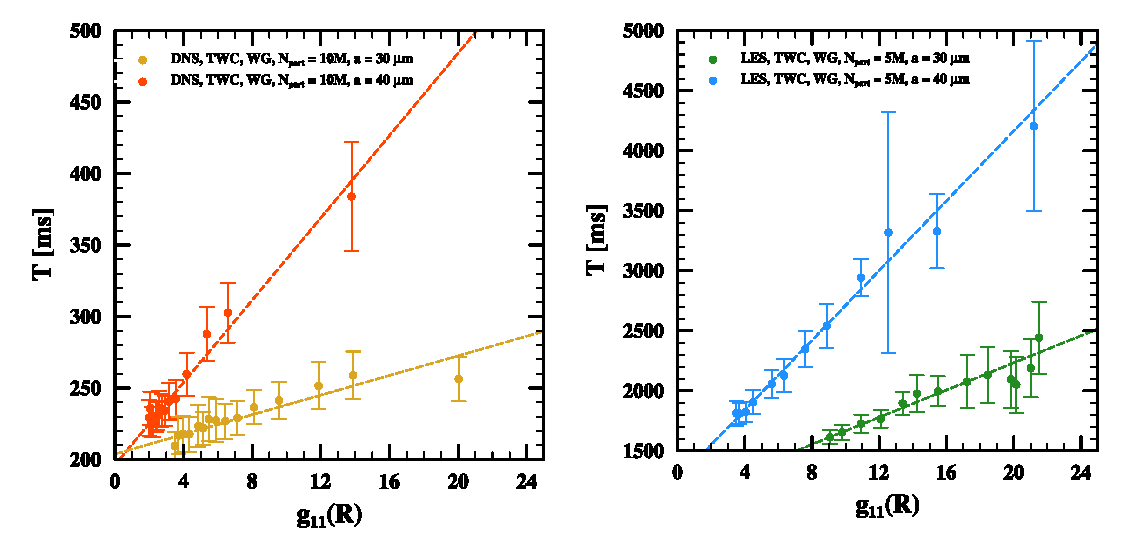
\includegraphics[width=13.5cm]{img/plots/3-2c-pfsrdf.pdf}
\caption{
Time-averaged wallclock times per step for DNS (left) and LES (right) simulations under two-way momentum coupling (TWC) with fixed number of computational particles (10M for DNS, 5M for LES) and radii ($30$, $40$~$\upmu\text{m}$), depending on the estimated values of the radial distribution function at contact range (RDF at $r=R$).
Dashed lines represent linear fit of included results weighted by~the~inverse variance of respective data points.
}
\label{fig:pfsrdf}
\end{figure}

Finally, the performance measurements that depend on less obvious parameter are presented, and that is the radial distribution function.
As outlined in Section \ref{ssc:ch2.coll.rdfrrv}, the RDF is meant as a statistical measure of preferential clustering of particles within the domain.
Statistically speaking, system with $g_{11}(r) = 1$ should exhibit almost uniform distribution of~particles, while higher values indicate increasing deviations from it, i.e. presence of more regions with high particle concentration (clusters) and emptier regions between them.
In the context of performance measurements and domain decomposition for parallel computation, this raises a question, whether such nonuniformity in particle distribution may affect simulation performance.
The broad analytical and experimental study of \textcite{Ayala2014} was performed under the assumption that simulated systems, on average, exhibit ``a reasonable computational load balance using a static domain decomposition parallelisation scheme''.
We~shall examine whether such hypothesis is admissible, especially for smaller grids used in this study, which may be more prone to nonuniformities in the particle distribution.

It was previously noted that there are stages during the processing of every time step that require global data synchronisation.
For that reason, the overall computational cost may be tied to the subdomain with the greatest number of particles being processed, as other processes eventually become idle waiting for such synchronisation.
As an initial hypothesis, we may expect more variance in distribution of particles among subdomains in simulations with higher RDF, resulting in worse performance.

Interestingly enough, the results presented in Figure \ref{fig:pfsrdf} seem to support such conjecture.
The WCT per step are plotted against estimated values of the RDF for DNS (left) and LES (right).
The timings for these plots were obtained from TWC simulations with the same number of computational particles and compared only within same particle radii, to eliminate influence on any other already observed dependencies.
The range of different values of the RDF were obtained by varying the super-particle parameterisation factor, $M$, which should have no direct bearing on computation times, while affecting the RDF via turbulence modulation (see~Figure~\ref{fig:twcrdfext}). 
Note that only simulations with gravity were used, and it might strengthen shown dependence.
This can be explained by the creation of elongated, column-like clusters of settling particles that are arranged in the same direction as subdomain ``pencils''.

It is apparent that execution times increase with rising values of the RDF. 
This is further clarified by dashed lines that represent linear fit of respective data points (weighted by their inverse variances). 
Furthermore, it seems that the slowdown rate may be related to the radius of particles being simulated, but more data for other radii would be required to unequivocally confirm such claim.

In general, these results show that some relation between the RDF and the distribution of particles in computational subdomains is present.
These two concepts, however, come from two different domains: the RDF is a continuous, statistical measure of certain physical properties of the system, while particle distribution is more technical measure, that depends on implementation details and discrete subdivision of computational domain.
Moreover, the~RDF is direction-agnostic while the distribution of particles in subdomains is anisotropic due to employed 2D domain decomposition scheme.
The relation between these two notions shall be~further explored in Section \ref{sc:ch3.perfp}.




\section{In-depth Code Performance Profile}
\label{sc:ch3.pprof}

In this section, the results of more detailed profiling of the code shall be presented.
For that purpose, each stage described in Table \ref{tab:code-steps} was separately timed in each parallel process and respective data was collected throughout 5 000 consequent iterations in the middle of the execution.
These results (per step), averaged over all processes and time steps considered, are denoted by  $T_i$, where $i \in \{ 1, \cdots, 10 \}$ refers to the specific stage that was timed (according to numbering introduced in Table \ref{tab:code-steps}).
Note, in particular, that $T_3 = T_{\text{TWC}}$ is the time spent on TWC-only computations, while $T_9 = T_{\text{LES}}$ -- for calculations of subgrid-scale model specific to LES.
Moreover, we define wallclock time measurements for the part of solver that is processing particles (Stages 2--6) and fluid flow (remaining stages), respectively, as follows
\begin{equation}
T_{\text{P}} = \sum_{i=2}^{6} T_i \, , \quad \quad \quad T_{\text{F}} = T - T_{\text{P}} \, ,
\label{eqn:pff-tp-tf}
\end{equation}
where $T$ is the average wallclock time of an entire step, as introduced in previous section (but, here, measured and averaged over all parallel processes, not just one).
Time spent on computations that involve droplets may be further subdivided into two parts: (1) devoted to the postprocessing of gathered statistics, $T_{\text{Pd}} = T_5$, and (2) associated with the particle solver (including calculations for the interphase momentum transfer), namely $T_{\text{Ps}} = T_{\text{P}} - T_{\text{Pd}}$.

\medskip

First, the focus is on the impact of LES on the computational performance of the fluid flow solver.
Relevant measurements were made for both ``standard'' DNS and LES, as well as for LES using grid size and division into subdomains typical for DNS in this study.
The~results are shown in Table \ref{tab:pff-flow}.
We may observe that the main computational burden of fluid simulation indeed rests in performing 3D FFTs ($T_8 + T_1$) which takes up around $85-90 \%$ of~the~time, regardless of the simulation type and grid size.
The grid size, however, greatly influences absolute time spent on FFT computations (due to theoretical complexity $\mathcal{O}(N^3 \log N^3)$) and, consequently, on the average total time of the fluid flow simulation step.
All of these timings are reduced approximately by the factor of $30$ when the grid size is reduced from $256$ to~$64$.
The fact that LES, due to inclusion of the subgrid-scale turbulence model, allows to~obtain comparable flow conditions with reduced $N$ is the main advantage of that method.
Furthermore, at least for the spectral-eddy viscosity SGS model, the additional cost of that modelling is almost negligible.
Also, it is clear that $T_{\text{LES}}$ has minimal ($\sim 2-3 \%$) impact on the complexity of the fluid flow processing.
The data shown in Table \ref{tab:pff-flow} comes from particle-free simulations, but the time spent on fluid flow computations is not affected by the inclusion of disperse phase.
Hence, these measurements are still viable for simulations with droplets, where respective contributions from $T_{\text{F}}$ are approximately constant. 

\begin{table}[h]
\centering
\scriptsize
\begin{tabular}{lcrrrrrr}
& & \multicolumn{1}{c}{Stage 7} &  \multicolumn{1}{c}{Stage 8} & \multicolumn{1}{c}{Stage 9} & \multicolumn{1}{c}{Stage 10} &  \multicolumn{1}{c}{Stage 1} & \multicolumn{1}{c}{TOTAL} \\
& & \multicolumn{1}{c}{Postprocessing} &  \multicolumn{1}{c}{FFT of $(\mathbf{u} \times \boldsymbol{\omega})$} &  \multicolumn{1}{c}{SGS model} &  \multicolumn{1}{c}{Flow eqns.)} & \multicolumn{1}{c}{2x $\text{FFT}^{-1}$} & \\
& $N$ & \multicolumn{1}{c}{$T_7$ [ms]} & \multicolumn{1}{c}{$T_8$ [ms]} & \multicolumn{1}{c}{$T_{\text{LES}}$ [ms]} & \multicolumn{1}{c}{$T_{10}$ [ms]} & \multicolumn{1}{c}{$T_1$ [ms]} & \multicolumn{1}{c}{$T_{\text{F}}$ [ms]} \\ \hline
\textbf{DNS} & \textbf{256} & $2.179 \pm 9.571$ & $18.027 \pm 1.457$ & --- & $6.676 \pm 0.371$ & $30.826$ & $55.708 \pm 10.934$ \\
LES & 256 & $2.193 \pm 9.633$ & $17.382 \pm 0.902$ & $1.501 \pm 0.265$ & $7.135 \pm 0.272$ & $31.768$ & $59.981 \pm 10.204$ \\
\textbf{LES} & \textbf{64} & $0.067 \pm 0.291$ & $0.571 \pm 0.055$ & $0.052 \pm 0.007$ & $0.155 \pm 0.008$ & $0.964$ & $1.808 \pm 0.337$ \\
\end{tabular}
\caption{Performance profile for simulations without particles.
Wallclock time measurements for~specific stages involved in fluid flow computations are shown for standard DNS and LES (in bold) as~specified in Table \ref{tab:perfs-params}.
Also results for LES performed with grid size ($256$) and subdomain division used in this study for DNS are shown for additional comparison.
}
\label{tab:pff-flow}
\end{table}

Note that some additional explanations are required for measurement uncertainties shown in~Table~\ref{tab:pff-flow}.
First of all, when $T_7$ is considered, recall that postprocessing stage is performed for simulations without particles only every 20 steps.
Moreover, most of the Stage 7 computations and I/O operations are confined to the single process.
Both of these circumstances result in high standard deviation since the averaging was applied both in time and across all processes.
More importantly, the uncertainties for $T_1$ were not shown, since they were artificially exaggerated due to the implementation details of the profile data collection process.
These artifacts manifest in higher variability between parallel processes in measurements for~the~first stage of every iteration, i.e. $T_1$.
Since Stage 1 consists of two 3D FFT calls, the~actual uncertainty associated with $T_1$ should be close to $2$ times that of $T_8$.
To eliminate this effect on~the~uncertainty of $T_{\text{F}}$ (here equal to $T$), the standard deviations shown here are taken from measurements for only single process, as for $T$ in Section \ref{sc:ch3.perfs}.  

\medskip

Figure \ref{fig:pffowcles} shows a graphical illustration of such profile data for OWC LES simulations.
At first glance, these profiles confirm several previous observations.
Firstly, the contribution from $T_\text{F}$ remains roughly constant for all simulations, irrespective of the presence of particles.
Furthermore, the fact that the computation cost of LES is dominated by stages devoted to~particles (see Figure \ref{fig:pfsowc}) is further validated here.
This remark may be quantified in terms of $T_{\text{P}} / T_{\text{F}}$ ratio, as displayed in Figure \ref{fig:pffowclesex} (left).
Since $T_{\text{F}}$ is approximately constant, such ratio is proportional to $T$.
Note that for LES these ratios, even for relatively small $N_{\text{part}} = 0.8 \, \text{M}$, attain considerable values.
Most notable here is the simulation with high inertia settling droplets ($a = 60$~$\upmu\text{m}$), in which case computations involving such meagre number of particles take (on average) around $15$ times more than those associated with the fluid flow.

\begin{figure}[h]
\centering
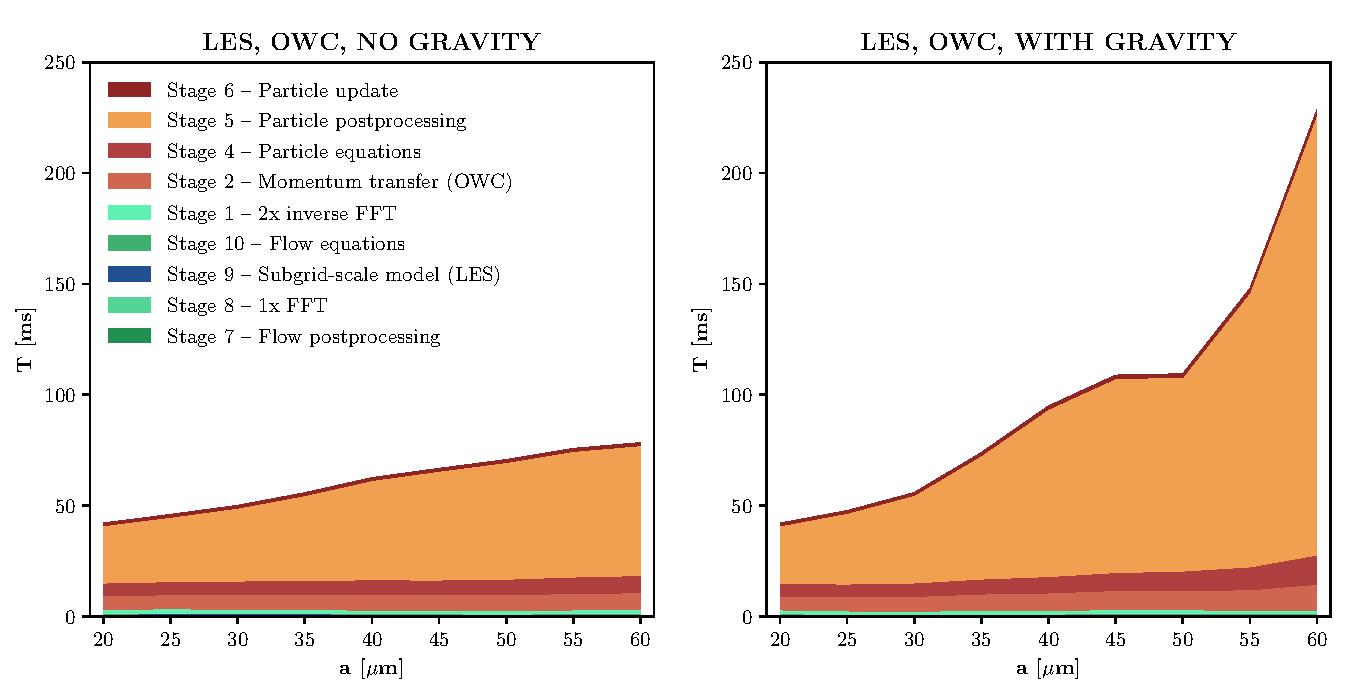
\includegraphics[width=13.5cm]{img/plots/3-3a-pffowcles.pdf}
\caption{
Performance profile for OWC LES simulations with and without gravity (right and left, respectively).
Layers of different colours represent average time per step for given stage ($T_i$) and~are~ordered as they appear in code.
For clarity, all stages related to the fluid flow computations are grouped together and represented by the bottom layers.
}
\label{fig:pffowcles}
\end{figure}

More significantly, introduced profile data permits a more in-depth study related to~the~separate stages of handling all computations involving particles.
In case of non-settling particles, the main reason for a slight increase in $T$ with growing droplet radii was hypothesised to~be~the~increasing size of halo regions involved in the processing of particle-pair statistics.
This conjecture appears to be correct, as we can clearly observe that $T_5 = T_{\text{Pd}}$ is entirely responsible for increasing wallclock times per step.
The remaining stages of particle solver ($T_{\text{Ps}}$) appear to be unaffected by changes in droplet radii.
This is entirely different for larger particles ($a > 30$~$\upmu\text{m}$) when effects of gravity are considered.
A more dramatic increase in the average iteration time is mainly due to growing $T_{\text{Pd}}$, as before, but other stages in particle solver are also affected.
As opposed to the postprocessing stage, the computational complexity of tasks in solver segment (Stages 2, 4 and 6) should be independent of the particle radii.
The chief factor influencing the computational complexity of these stages is the number of~particles in each subdomain.
These should remain constant, unless we consider nonuniformities in particle distribution among subdomains.
On that note, relatively large uncertainties of~presented quantities (see Figure \ref{fig:pffowclesex}) indicate high variability of stage timings that, in turn, maybe related to the aforementioned nonuniformities.

\begin{figure}[h]
\centering
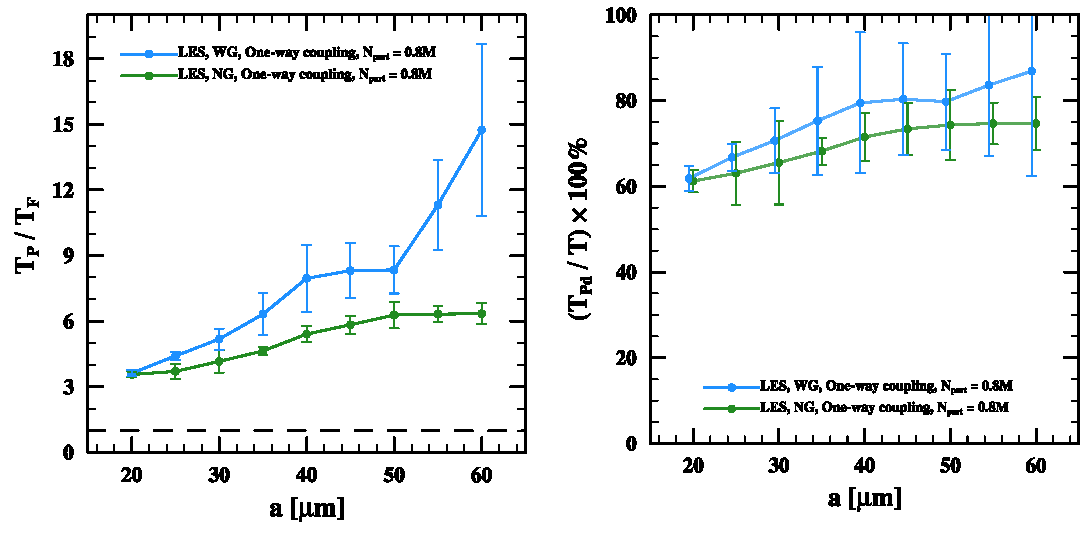
\includegraphics[width=13.5cm]{img/plots/3-3b-pffowclesex.pdf}
\caption{
The ratio of average wallclock times spent on processing particles, $T_{\text{P}}$, and the fluid flow, $T_{\text{F}}$ (left); and average percentage of overall wallclock time per step occupied by particle postprocessing tasks, $(T_{\text{Pd}} / T)$ (right), for OWC LES with and without gravity.
Plots on the right have slight horizontal offset added to make uncertainty bars more visible.
}
\label{fig:pffowclesex}
\end{figure}

These profiles (Figure \ref{fig:pffowcles}) show preeminence of computational costs associated with particle processing in LES, as suggested before.
Even more specifically, such effort is concentrated, for the most part, on the postprocessing of their statistics.
This hypothesis is quantified in~terms of average percentage of iteration that processes are occupied with tasks specific for~Stage 5, as shown in Figure \ref{fig:pffowclesex} (right).
In general, these percentages follow similar trends as the overall average step times, i.e. increase with droplet radii and such increase is more pronounced for the settling particles.
More specifically, at least for LES, particle postprocessing accounts for roughly $60-85 \%$ of the entire time step duration across processes,  which is indeed a significant value.
In more practical terms, that particular stage seems to be the main bottleneck that most deserves further examination and more attention in any optimisation efforts.  

\begin{figure}[h]
\centering
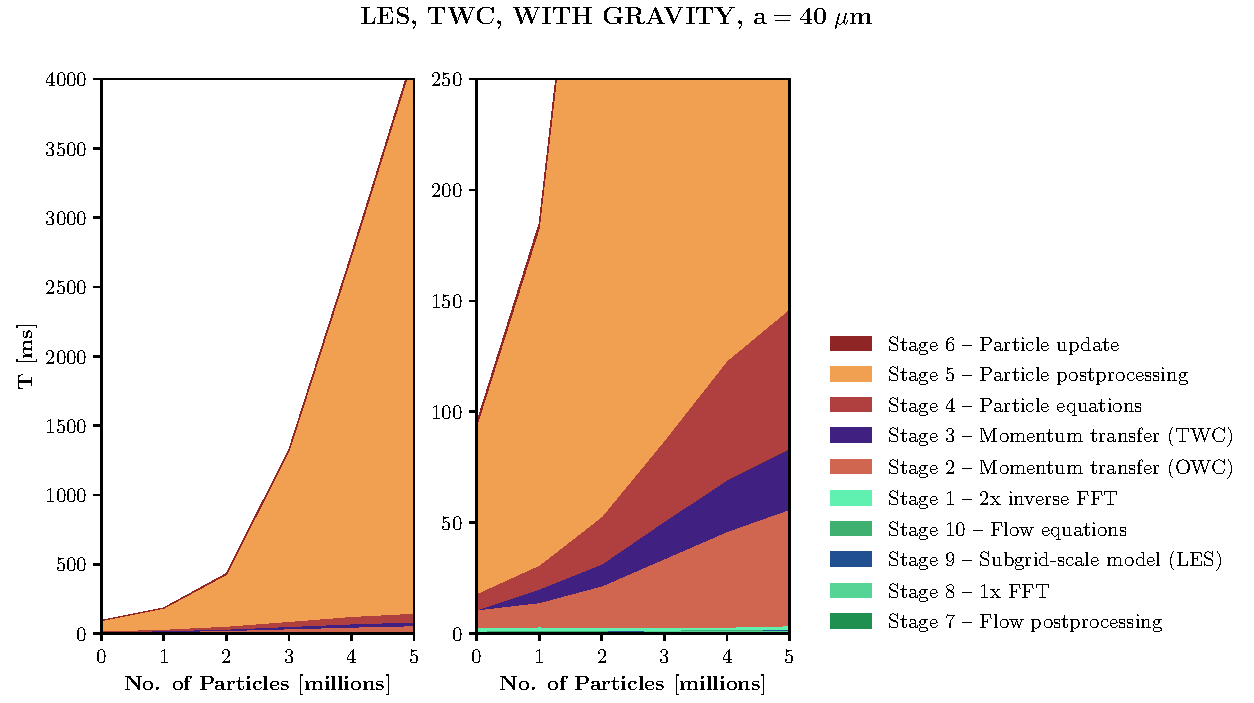
\includegraphics[width=13.5cm]{img/plots/3-3c-pfftwcles.pdf}
\caption{
Performance profile for TWC LES simulations with gravity for droplets with $40$~$\upmu\text{m}$ radius.
Consistent with Figure \ref{fig:pffowcles}.
Both plots present profiles for the same simulations, but the one on the right focuses on smaller range on the $Y$-axis to ``magnify'' data pertaining to timings other than $T_5$ ($ = T_{\text{Pd}}$).
The left profile ($0$ on $X$-axis) was given for corresponding OWC simulation with~$N_{\text{part}} = 0.8\text{M}$. 
}
\label{fig:pfftwcles}
\end{figure}

These conclusions are even more compelling when we consider a similar profile for TWC LES, where more particles were simulated (although still below 5 million).
The relevant data is shown in Figure \ref{fig:pfftwcles}.
Previously (see Figure \ref{fig:pfstwc}) it was pointed out that the computational cost of LES blows up at even moderate increase of $N_{\text{part}}$.
It was attributed to the larger share of particles that each process has to deal with, since the total number of subdomains is reduced $4$-fold with respect to DNS (see Table \ref{tab:perfs-params}).
The rate of this increase, however, was greater than anticipated, and we can conclude that it is not merely due to larger computational burden for the particle solver, but predominately due to the postprocessing stage.
Since the main goal of this study requires collection of the particle-pair statistics, the effort required for such calculations approximately scales with the square of the number of particles per subdomain (for more details, see theoretical analysis in Appendix C of \textcite{Ayala2014}).
Still, even this explanation is not enough to account for such enormous increase.
Such insight, however, is sufficient to explain that $T_{\text{Pd}}$ becomes dominant contributor to each time step not only for~LES but also for DNS when $N_{\text{part}}$ becomes large enough.

\begin{figure}[h]
\centering
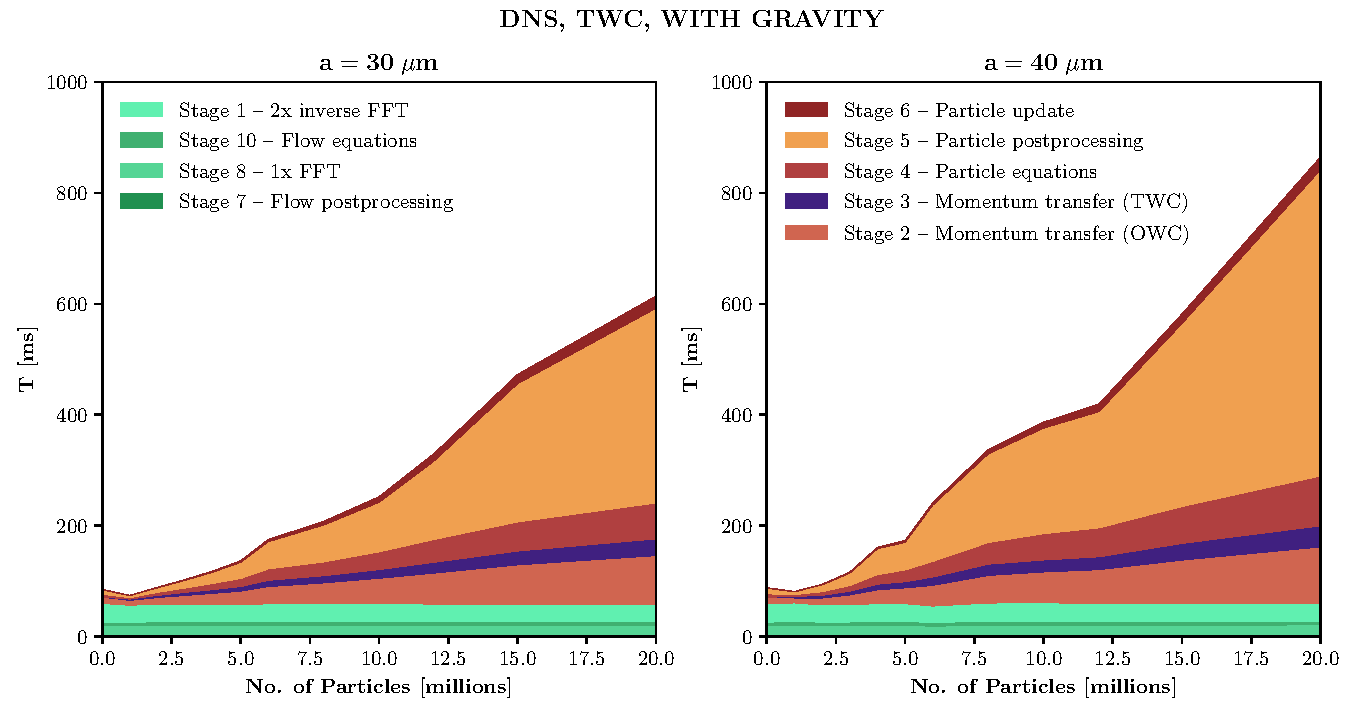
\includegraphics[width=13.5cm]{img/plots/3-3d-pfftwcdns.pdf}
\caption{
Performance profile for TWC DNS simulations with gravity for droplets with radii $30$~$\upmu\text{m}$ (left) and $40$~$\upmu\text{m}$ (right).
Consistent with Figures \ref{fig:pffowcles} and \ref{fig:pfftwcles}.
}
\label{fig:pfftwcdns}
\end{figure}

The profile data for TWC DNS is shown in Figure \ref{fig:pfftwcdns}.
It provides a great opportunity to extend above considerations to a wider range of $N_{\text{part}}$ (1 to 20 million).
Firstly, we can observe that computations involving fluid flow occupy a significant part of the entire DNS iteration.
In fact, for $N_{\text{part}}$ smaller than around 5-6 million they take up greater portion of~the~entire step time than those devoted to particles.
This observation is further confirmed by data in Figure \ref{fig:pfftwcex} (left) where respective $(T_{\text{P}} / T_{\text{F}})$ ratios are plotted.
Note that it was necessary to use log scale to accommodate these ratios for LES which are roughly two orders of magnitude larger than for DNS (for equal $N_{\text{part}}$).
For $N_{\text{part}} > 6$ million, tasks involved in~particle computations take the majority of step time even for DNS and that ratio grows with increasing number of~particles in the system.
Such increase, however, is not overwhelming as in case of LES where, at least for relatively small, feasible values of $N_{\text{part}}$, obtained ratios appear to be growing exponentially.

\begin{figure}[h]
\centering
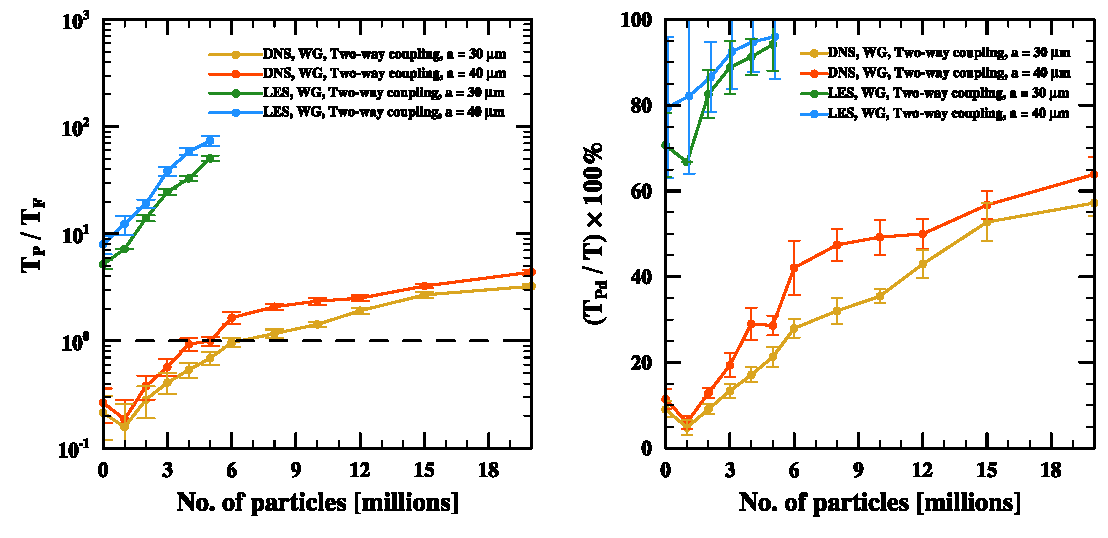
\includegraphics[width=13.5cm]{img/plots/3-3f-pfftwcex.pdf}
\caption{
The ratio of average wallclock times spent on processing particles, $T_{\text{P}}$, and the fluid flow, $T_{\text{F}}$ (left, linear-log scale); and average percentage of overall step time occupied by particle postprocessing tasks, $(T_{\text{Pd}} / T)$ (right), for TWC simulations with gravity.
Plots for LES on the right have slight horizontal offset added to make uncertainty bars more visible.
}
\label{fig:pfftwcex}
\end{figure}

Figure \ref{fig:pfftwcex} (right) shows percentages of time taken by particle postprocessing for TWC simulations with increasing number of particles.
The results for LES verify previous remarks on the immense predominance of $T_{\text{Pd}}$ over average times taken by other stages.
The portion of time taken up by particle postprocessing for the most part exceeds $90 \%$ and grows with increasing $N_{\text{part}}$ approaching $100 \%$.
When DNS is considered, the picture is much more varied.
For relatively small particle counts the influence of Stage 5 on the overall code performance is limited, although it quickly becomes more prominent for moderately sized droplet populations ($3-6$ million).
In simulations at larger mass loadings, the time consumed by the postprocessing of particle statistics reaches and even exceeds $50 \%$, although the rate of such increase becomes smaller.
Thus, the postprocessing stage is not only the bottleneck for LES but also for DNS when larger numbers of droplets need to be simulated (and this is vital to~obtain relevant results for simulations under two-way momentum coupling).  

The profile data for DNS (Figure \ref{fig:pfftwcdns}), thanks to wider range of particle counts considered, provide deeper insight into the growth of average computational costs associated with different stages of droplet processing.
As it was elaborated earlier, the main reason for the overall increase in average step times with rising $N_{\text{part}}$ is $T_{\text{Pd}}$ that scales, at best, with the square of the number of particles in subdomain.
This expansion is clearly visible in the profile plot.
The rate of $T_{\text{Pd}}$ increase, however, is not steady and it appears to slow down with growing $N_{\text{part}}$.
These irregularities cannot be explained at this point but may provide another hint at the influence of the nonuniformities in particle distribution among subdomains on~the~computational performance.

\begin{figure}[h]
\centering
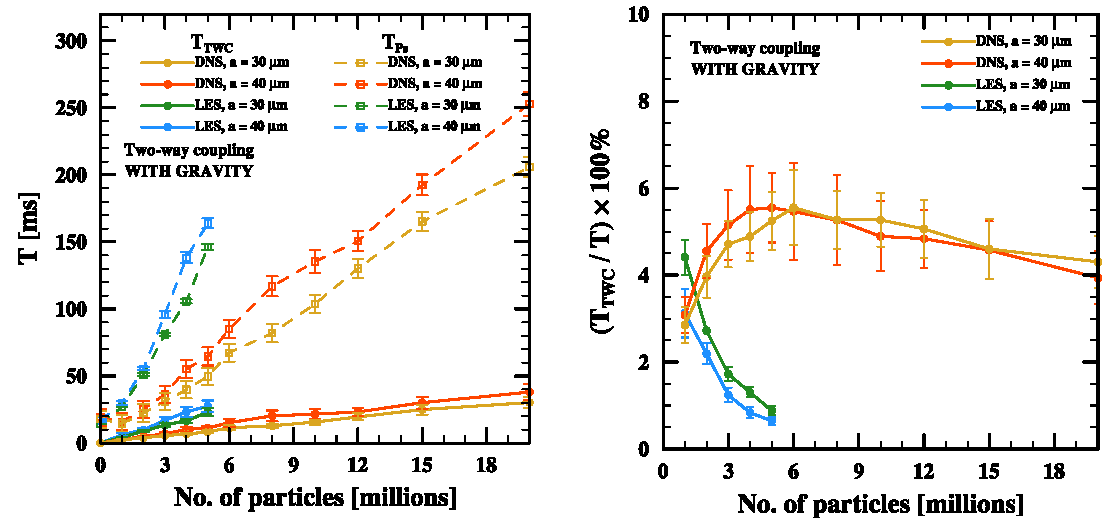
\includegraphics[width=13.5cm]{img/plots/3-3e-pfftwctwc.pdf}
\caption{
Time- and process-averaged wallclock times of TWC-specific stage, $T_{\text{TWC}}$, and all stages of the particle solver, $T_{\text{Ps}}$ (dashed line; left); and average percentage of $T_{\text{TWC}}$ as part of the~entire step time.
All data shown for TWC simulations with gravity and as a function of the number of particles in the system.
}
\label{fig:pfftwctwc}
\end{figure}

When we focus only on the stages associated with the particle solver and their average wallclock time, $T_{\text{Ps}}$, its increase is roughly linear with respect to $N_{\text{part}}$ (for DNS).
This is somewhat true for LES as well, although the amount of data is not sufficient to fully validate such claim.
This relation is presented in Figure \ref{fig:pfftwctwc} (left, dashed line).
The growth of $T_{\text{Ps}}$ for DNS shows some interesting fluctuations that, up to a point, may be related to trends exhibited by the RDF for corresponding simulations (see Figure \ref{fig:twcrdf}, bottom left).
These variations, however, are small enough to fall within the scope of measurement uncertainties, hence any direct correlation is hard to establish at that point.

This study is a good opportunity to ascertain the impact of calculations specific to TWC simulations on their overall computational performance.
Previously it was intimated that such effect is relatively limited, and the main cause for more burdensome nature of these simulations does not lie in these additional calculations, but higher mass loadings that are necessary to make effects of two-way momentum coupling fully appreciable.
Results shown in Figure \ref{fig:pfftwctwc} confirm such claim.
The plot on the left shows absolute mean values of $T_{\text{TWC}}$ for simulations with gravity.
Both in case of DNS and LES it increases linearly with growing number of particles and constitutes relatively small fraction ($\sim 0.15$) of the overall time consumed on particle calculations (excluding postprocessing).
To further ascertain relatively small influence of these additional TWC-specific computations on the average overall step time, respective percentages are presented in Figure \ref{fig:pfftwctwc} (right).
For LES, $T_{\text{TWC}}$ quickly becomes negligible due to huge costs of the particle postprocessing that overwhelm influence of any other stages.
Similar effect, although to a much lesser degree, may be observed for DNS with larger mass loadings ($N_{\text{part}} \ge 6$ million), where $T_{\text{TWC}}$ starts to lose significance compared to rapidly growing $T_{\text{Pd}}$.
Nevertheless, for DNS the percentage of computational effort spent on~Stage 3, where momentum transfer from particles to the fluid is calculated, ranges between $3 \%$ and~$6 \%$.
This is a relatively minor contribution to the numerical complexity of entire simulation.
Interestingly, as Figure \ref{fig:pfftwctwc} (left) indicates, it may often be more impactful to~change particle radii from $30$~$\upmu\text{m}$ to $40$~$\upmu\text{m}$ than to enable two-way momentum coupling (assuming $N_{\text{part}}$ remains unchanged).

As a side note, we may observe, that the average time spent on the actual update of~particle positions, $T_6$, is the smallest chunk of $T_{\text{Ps}}$.
The most effort in that phase boils down to the interprocess communication responsible for relocation of particles between processes when they cross physical boundaries of respective subdomains.
This implementation of the solver uses the direction of gravity which is aligned with subdomain ``pencils'' exactly for that reason, i.e. to minimise occurrences of droplets moving from one subdomain to the other \parencite{Ayala2014}.
Note, that $T_6$ is even smaller, almost negligible, for LES (see Figures \ref{fig:pffowcles} and \ref{fig:pfftwcles}).
This is due to the coarser subdivision of entire domain which makes such crossing events, and~necessary data transfer associated with them, even rarer.

\medskip

Moreover, an additional effort was made to account for all the time during each iteration that was spent on interprocess communication via respective MPI calls (see Section \ref{sc:ch3.perf}).
These measurements, however, do not differentiate between the time of an actual data transfer and waiting for other processes to facilitate such communication.
Moreover, they do not account for the MPI calls that are part of the transpose operations involved in the parallel implementation of the 3D FFT (its implementation, is treated in this context as separate, self-contained dependency).
Such timings, averaged over all processes and iterations, are denoted as $T_{\text{comm}}$ and shown in Figure \ref{fig:pffcomm}.

\begin{figure}[h]
\centering
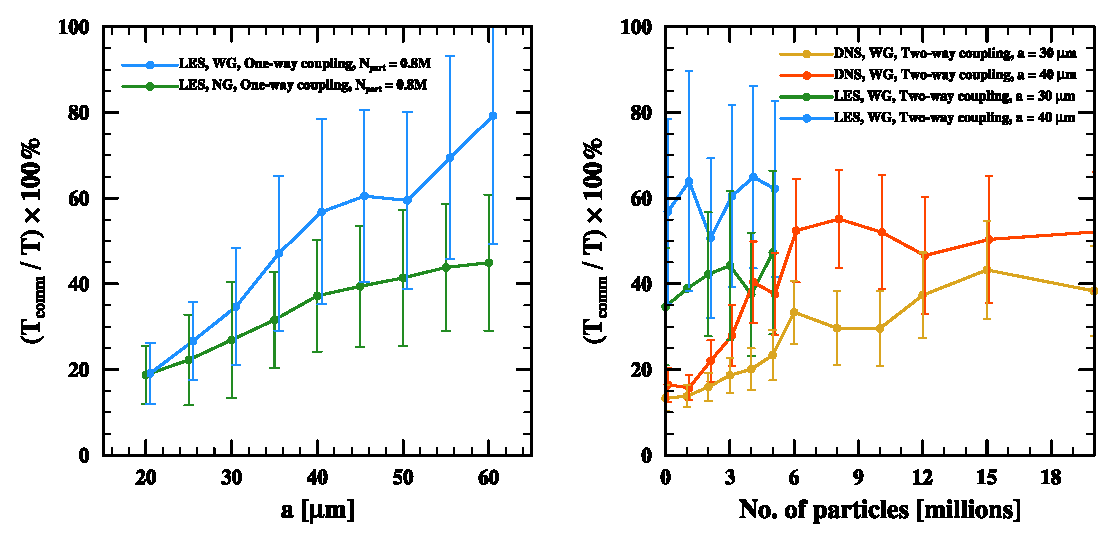
\includegraphics[width=13.5cm]{img/plots/3-3g-pffcomm.pdf}
\caption{
Average percentage of wallclock time per step spent on interprocess communications (outside of 3D FFT) for OWC LES (left) and TWC (right) simulations.
}
\label{fig:pffcomm}
\end{figure}

Firstly, it needs to be mentioned that all measurements shown in Figure \ref{fig:pffcomm} are burdened with relatively high uncertainties.
Such variance may be, at least to some degree, attributed to the process of averaging across all parallel processes.
When one process initialises communication and waits for another one (or many) to complete its computations, the difference between their contribution to $T_{\text{comm}}$ increases.
This is a common, though undesirable, occurrence and this fact is reflected in the considerable standard deviations associated with $T_{\text{comm}}$.
Even further, such uncertainties (at least for the sake of relative comparisons) may serve as an indirect measure of the wallclock time spent on waiting for communication and not performing actual data transfer.
Still, such interpretation, as well as any analysis of presented results requires additional caution.

Taking all this into account, we may formulate few conjectures on that basis.
First, the proportion of time spent on communication (whether active or idle) is significant.
This is especially true for TWC LES and TWC DNS with larger numbers of particles being simulated.
In case of OWC LES, this contribution increases with droplet radii, more rapidly when gravity is considered.
For exactly these simulations we have already observed a significant impact of~$T_{\text{Pd}}$ on the average time of the entire step.
Also trends followed by both ratios, i.e.~$(T_{\text{comm}} / T)$ and $(T_{\text{Pd}} / T)$, appear somewhat similar.

This indirect relation between $T_{\text{comm}}$ and $T_{\text{Pd}}$ is probably related to the nature of communication that is required by Stage 5.
One part of the picture is the exchange of particle data from the halo regions.
It partly explains the dependence of $T_{\text{comm}}$ on the particle radii, but it is not enough to produce observed dependence.
More importantly, at the end of that stage, a~final synchronisation between all processes is necessary to transfer all results of postprocessing to one specified process responsible for writing data to the storage.
Assuming that there are some differences between the number of particles in subdomains, all processes in the end have to wait for one of them that has the largest workload.
This variance in the time spent on computations, presumably associated with differences in the particle count between processes, is further exacerbated by the quadratic complexity of particle-pair statistics calculations.
These conclusions are based on indirect evidence and need further justification.
That, however, would require more granular measurements for the communication times, e.g.~$T_{\text{comm}}$ statistics collected individually per stage or separate accounting of time actively spent transferring data between processes and idly waiting for others.
This level of detail, however, is~beyond the scope of this study.

\medskip

\begin{figure}[h]
\centering
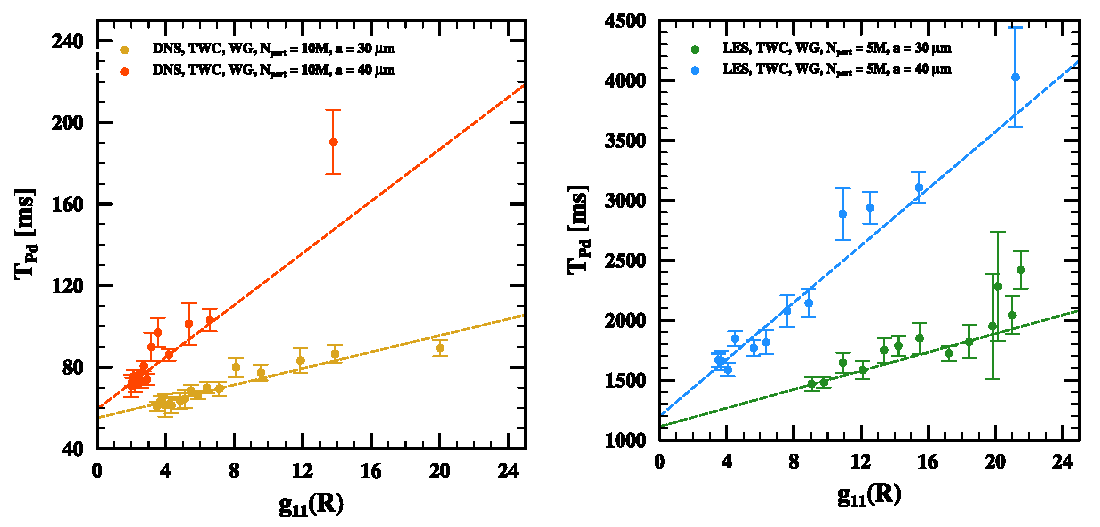
\includegraphics[width=13.5cm]{img/plots/3-3h-pffrdfpd.pdf}
\caption{
Time- and process-averaged wallclock times of particle postprocessing stage per step for DNS (left) and LES (right), depending on the estimated values of the radial distribution function at contact range (RDF at $r=R$).
Consistent with Figure \ref{fig:pfsrdf}.
}
\label{fig:pffrdfpd}
\end{figure}

Finally, as a continuation of analyses started in previous section (see Figure \ref{fig:pfsrdf}), the influence of particle distribution between subdomains on computational performance shall be further examined.
This is in line with conclusions from previous paragraph, suggesting that deficiencies in computational performance of some simulations may be due to nonuniformity of~that~distribution which causes excessive waiting times for final synchronisation after particle postprocessing stage.

Figures \ref{fig:pffrdfpd} and \ref{fig:pffrdfps} illustrate the dependence of $T_{\text{Pd}}$ and $T_{\text{Ps}}$, respectively, on the estimated RDF at contact distance for TWC simulations with settling particles.
All plots were made in a similar way to those in Figure \ref{fig:pfsrdf} (where overall step time, $T$, was considered).
According to expectations,  $T_{\text{Pd}}$ is highly sensitive to the RDF and plots presented in Figures \ref{fig:pfsrdf} and \ref{fig:pffrdfpd} show many similarities.
As before, the rate of increase of $T_{\text{Pd}}$ with respect to~the~RDF is consistently higher for droplets with higher radius (for both DNS and LES).  
The~only difference is the tendency for $T_{\text{Pd}}$ results to fall above linear fit line for higher values of $g_{11}(R)$.
It may be attributed to the fact that quadratic dependence on the number of~particles in the subdomain gains more prominence when $T_{\text{Pd}}$ is considered.

\begin{figure}[h]
\centering
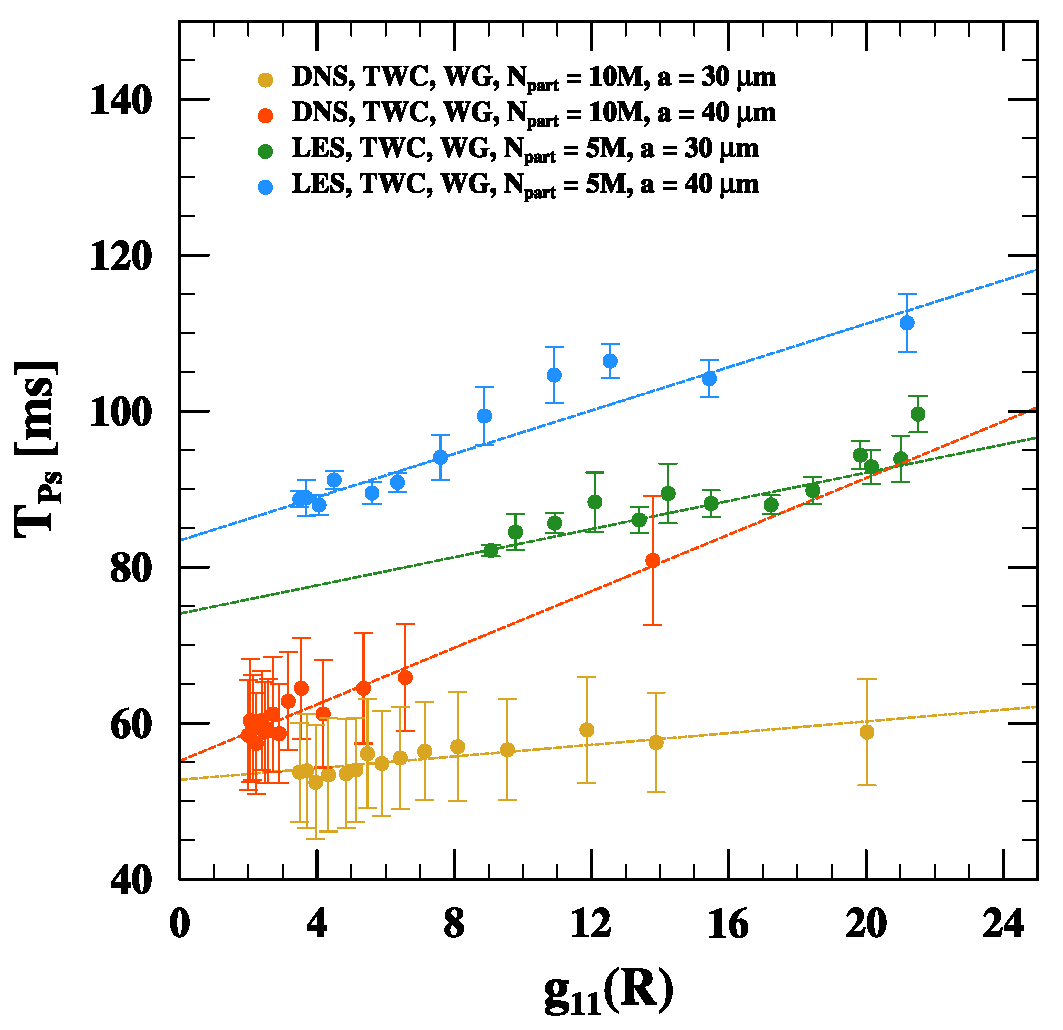
\includegraphics[width=8cm]{img/plots/3-3i-pffrdfps.pdf}
\caption{
Time- and process-averaged wallclock times of particle solver stages per step for DNS and LES, depending on the estimated values of the radial distribution function at contact range (RDF at $r=R$).
Consistent with Figure \ref{fig:pfsrdf}.
}
\label{fig:pffrdfps}
\end{figure}

The results shown in figure \ref{fig:pffrdfps} serve to further establish the hypothesis that increased variance in the distribution of particles among processes (associated with the Stokes number and higher values of the RDF) mainly affects computational complexity of the entire simulation via its impact on the particle postprocessing stage.
It shows that timings related with the solver stages (for particles) exhibit considerably weaker sensitivity to the RDF than $T_{\text{Pd}}$.
Some influence here is expected and observed, but in absolute terms it does not have as striking impact on the overall wallclock times per step.
The most peculiar example here is the case of DNS with $a = 30$~$\upmu\text{m}$, where almost no influence of the RDF on $T_{\text{Ps}}$ is observed.
For completeness, note that only remaining section of the code (timing-wise) not accounted for in Figures \ref{fig:pffrdfpd} and \ref{fig:pffrdfps} is the part responsible for the fluid flow computations.
As shown before, however, $T_{\text{F}}$ is roughly constant for all simulations of the same type, hence it clearly does not demonstrate any dependence on the RDF.

These section have repeatedly shown that nonuniformities in particle distribution between subdomains may indeed have significant bearing on the computational costs of simulations in~question.
Moreover, these effects seem to manifest for the most part in the stage where postprocessing of particle-pair statistics is performed (Stage 5).
This claim, however, needs more granular profile data, especially when it comes to interprocess communication, for more direct validation.
In the following section, though, another approach to that important question shall be taken.

 

\section{Distribution of Particles in Computational Subdomains and Its Effect on Performance}
\label{sc:ch3.perfp}


The aim of this section is to address the hypothesis that the distribution of particles among subdomains may have significant impact on the computational performance of simulations.
Such notion was appearing throughout this chapter mainly in two contexts.
Firstly, it was shown that there is a correlation between the average wallclock times of the entire iteration (and, in particular, of the particle postprocessing stage) and the RDF (see Figures \ref{fig:pfsrdf} and \ref{fig:pffrdfpd}).
The RDF is related to particle accumulation, yet it is a continuous physical statistic that cannot be directly translated to discrete and implementation-driven parameter that is of~interest at this point.
Moreover, the RDF measures local density of particle pairs \parencite{Grabowski2013}, particularly when it is considered at contact distance.
Here, this locality is understood to include much smaller ranges than physical dimensions of the entire subdomain.   
Secondly, the differences between particle counts in individual processes may explain larger than expected impact of the particle postprocessing stage on the computational complexity of~simulations.
This may be due to the final synchronisation of all processes at the end of~Stage~5 that ties the performance of the entire simulation to the efficiency of the most particle-laden process at any given time step.
Also, the quadratic dependence of these calculations on the number of particles in subdomains exacerbates such effect.
Still, the above evidence is only cursory and more direct approach is required.

For that reason, the counts of computational particles assigned to each parallel process were collected for the entire duration of the simulation in question (every 5 time steps).
To~simplify further discussion the following notation is introduced.
Let $\#SD$ be the number of subdomains (or, equivalently, individual parallel processes -- $N_{\text{proc}}$) that entire domain is divided into.
It is based on the 2D decomposition where two chosen axes are uniformly divided into $(\#SD_{\text{ax}})$ sections, therefore $\#SD = \left( \#SD_{\text{ax}} \right)^2$.
The particle count at given time step $t$ and for process associated with subdomain $(i,\,j)$ is denoted by $\mathcal{N}_{(i,\,j)}(t)$, where $i,\,j \in \{ 1, \, \ldots , \, \#SD_{\text{ax}} \}$.
Note, that the total number of particles in the system, $N_{\text{part}}$, and the subdomain count remain fixed for the entire simulation.
For that reason, the mean number of particles per subdomain is well-defined for any execution and is constant, i.e. we have
\begin{equation}
\langle \mathcal{N}_{(i,\,j)}(t) \rangle \; = \; \frac{N_{\text{part}}}{\#SD} \; := \; \mathcal{N} \; = \; \text{const} \, .
\label{eqn:pfp-avg}
\end{equation}
To characterise the degree of nonuniformity of the particle distribution in subdomains we employ two statistics: (1) $\sigma_{\mathcal{N}}(t)$ -- the standard deviation of particle counts from all subdomains for a given time step $t$; and (2) $\max_{i,\,j}\{\mathcal{N}_{(i,\,j)}(t)\}$ -- the maximal number of particles among all subdomains at $t$.
The former measure of the variance of distribution is self-explanatory.
As for the latter, it is mainly motivated by the fact that when the synchronisation of parallel processes is considered the performance should be tied to the process with the maximal computational workload.
For more concise presentation, both statistics were averaged over the~entire timespan of the simulation (denoted: $\langle \sigma_{\mathcal{N}} \rangle$ and $\langle \mathcal{N}_{\max} \rangle$, respectively) and normalised by the average number of particles per subdomain, $\mathcal{N}$.

\medskip

First, the previously established relation between the RDF at contact distance and $T$ (or~$T_{\text{Pd}}$) is examined.
Figure \ref{fig:pfprdf} (top and middle row) show that indeed there is a degree of correlation between respective statistics introduced above and the RDF.
Interestingly, the correspondence between these parameters is very similar to that between   $g_{11}(R)$ and $T$ (see~Figure~\ref{fig:pfsrdf}), as we observe that both values and the rate of their increase as a function of the RDF depends on the droplet radius.
Also, for the most part, the average $\mathcal{N}_{\text{max}}$ is limited to well below $2 \mathcal{N}$ which represents a relatively small variance, especially considering that the respective values of the RDF may differ by a factor of $6$.
Thus, even though there is a relation between the RDF and the nonuniformity of particle distribution in subdomains, it appears to~be~weaker than anticipated.

\begin{figure}[!htbp]
\centering
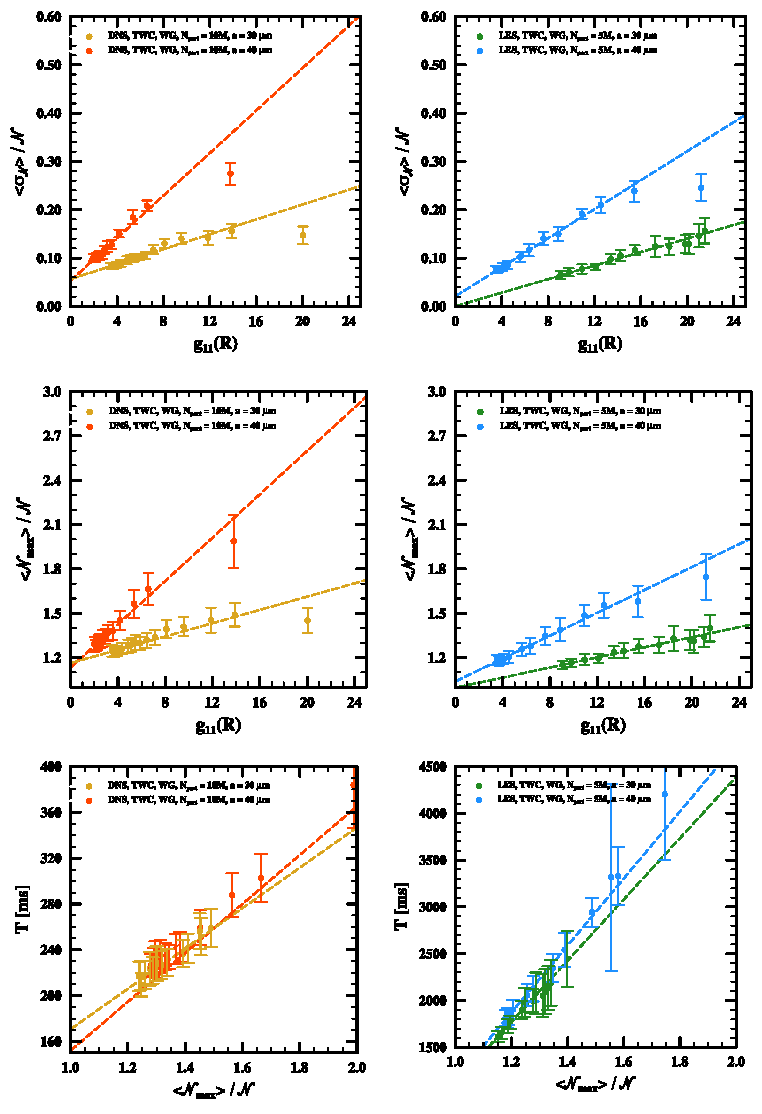
\includegraphics[width=13.5cm]{img/plots/3-4a-pfprdf.pdf}
\caption{
Correlation between the RDF at contact distance and particle distribution statistics: time-averaged standard deviation, $\langle \sigma_{\mathcal{N}} \rangle$ (top), and maximal particle count, $\langle \mathcal{N}_{\max} \rangle$, normalised by average number of particles per subdomain for DNS (left) and LES (right).
Also correlation between normalised maximal particle counts and average step times, $T$, was included (bottom).
Consistent with Figure \ref{fig:pfsrdf}.
}
\label{fig:pfprdf}
\end{figure}

The bottom plots in Figure \ref{fig:pfprdf} show average wallclock times per step, $T$, in relation to the average normalised maximal particle counts in subdomains for the same set of simulations.
It is clear that the relationship between these two statistics is much more direct.
Most importantly, there is no additional dependence on the droplet radius.
This shows that indeed the variance of particle distribution between parallel processes has direct impact on the computational costs of simulations.
Note that the same relation also holds when $\mathcal{N}_{\max}$ is replaced by average standard deviations (not shown).
In general, both statistics introduced here to measure the nonuniformity of particle distribution between subdomains are highly correlated, and may be used almost interchangeably.

Even though the increase of distribution statistics is the same for both DNS and LES, in~case of LES the absolute increase of $T$ is much faster.
This is due to the adopted normalisation.
For simulations involved in Figure \ref{fig:pfprdf} the average particle count per process is two times larger for LES (here $\mathcal{N}_{\text{DNS}} \approx 39\text{k}$ and $\mathcal{N}_{\text{LES}} \approx 78\text{k}$).
Thus, even for the same values of $(\mathcal{N}_{\max} / \mathcal{N})$, the actual computational burden of the particle solver is two times larger as well (not to mention much larger increase for the particle postprocessing tasks due to quadratic dependence on $\max_{i,\,j} \mathcal{N}_{(i,\,j)}(t)$ at each time step $t$).

As a side note, in top and middle plots in Figure \ref{fig:pfprdf} we may observe individual data points for larger values of the RDF that do not follow trend set by the remaining values.
They all fall below the line obtained by a linear fit performed as in Figure \ref{fig:pfsrdf}.
This is more pronounced when standard deviation is considered.
Interestingly, simulations represented by these outlier results are the only ones that were not subject to the superparticle parameterisation ($M=1$).
Furthermore, such difference is observed only between simulations where $M = 1$ and $M > 1$, but not when they differ in $M$ as long as it is greater than $1$.
\textcite{Rosa2022} analyse influence of the superparticle factor, $M$, on the $g_{11}(R)$, but it is gradual unlike in this case.
Thus, it is not clear in what way the higher values of $M$ could affect statistics considered here to introduce such peculiarity.
This issue, however, is beyond the scope of this study and~requires further investigation. 

\begin{figure}[h]
\centering
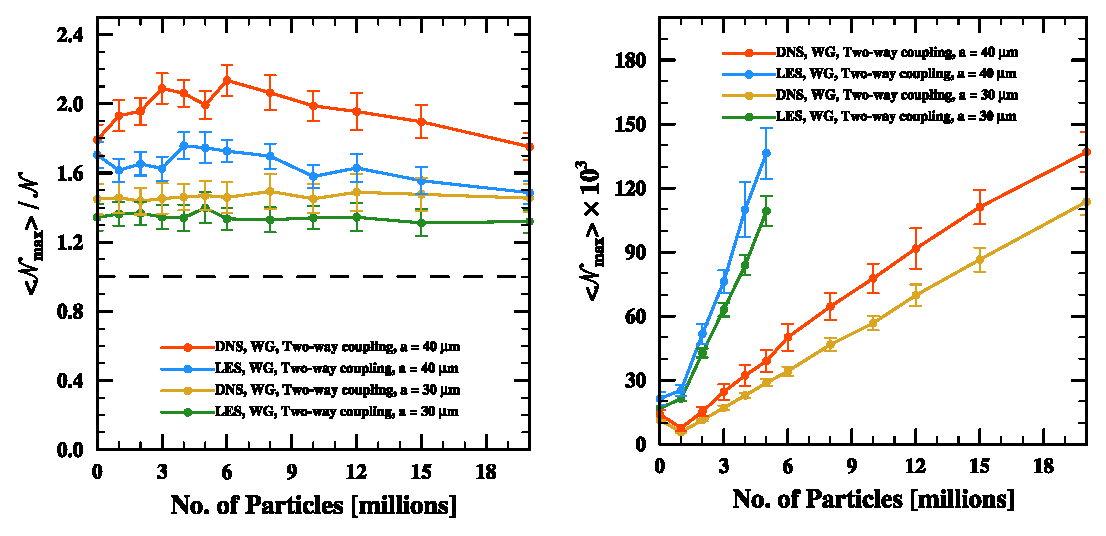
\includegraphics[width=13.5cm]{img/plots/3-4b-pfptwc.pdf}
\caption{
Time-averaged maximal number of particles in subdomains, $\langle \mathcal{N}_{\max} \rangle$, for TWC simulations with gravity (DNS and LES).
On the left, values are normalised by the average number of~particles per subdomain; on the right, absolute values are given (in thousands of particles).
}
\label{fig:pfptwc}
\end{figure}

For broader picture, Figure \ref{fig:pfptwc} (left) shows normalised maximal numbers of particles in~subdomains for TWC simulations with gravity.
Again, we observe that for the most part such maximums are not greater than $2 \mathcal{N}$.
Also, they are weakly sensitive to the total number of particles in the system.
In fact, for droplets with radius $30$~$\upmu\text{m}$ normalised $\langle \mathcal{N}_{\max} \rangle$ remains almost constant when $N_{\text{part}}$ changes.
When we compare these results with respective estimates for the RDF (see Figure \ref{fig:twcrdf}, bottom) they can be related to the changes in the clustering behaviour of particles.
Not only the RDF is almost constant with $N_{\text{part}}$ for $a = 30$~$\upmu\text{m}$, but for $a = 40$~$\upmu\text{m}$ it decreases monotonically which is reflected in steady decrease of average maxima for $N_{\text{part}} > 6$ million.
On the other hand, the increase of $\langle \mathcal{N}_{\max} \rangle / \mathcal{N}$ for DNS with $a = 40$~$\upmu\text{m}$ and smaller mass loadings cannot be expressed in terms of the changes in the RDF, and require additional investigation.
Still, these results explain trends in $T$ and $T_{\text{Pd}}$ for~these simulations (see Figures \ref{fig:pfftwcdns} and \ref{fig:pfftwcex}), further showing the significance of the particle distribution among processes when analysing the computational costs of simulations.
Also, it~is~important to observe, in general, that droplet radius has more impact on $\langle \mathcal{N}_{\max} \rangle / \mathcal{N}$ than $N_{\text{part}}$ (or, indirectly, $g_{11}(R)$).

Note that above discussion pertains to the values of $\langle \mathcal{N}_{\max} \rangle$  that are normalised by $\mathcal{N}$ which changes proportionally to $N_{\text{part}}$.
Figure \ref{fig:pfptwc} shows the absolute values of respective maxima (in thousands of particles).
This picture is more appropriate when the computational complexity of simulations is concerned, as these numbers actually approximate the burden of calculations for the most particle-laden process.
This difference is clearly visible for LES.
Even though normalised maxima for DNS and LES follow similar trends, when it comes to absolute counts they are considerably higher for LES (approximately by the factor of $4$ due to difference in $\#SD$).

Figure \ref{fig:pfpowc} shows particle distribution statistics when simulations under one-way momentum coupling is considered.
The familiar trends (see Figures \ref{fig:pfsowc} and \ref{fig:pffowclesex}) may be observed in both cases, as $\langle \sigma(\mathcal{N}) \rangle / \mathcal{N}$ and $\langle \mathcal{N}_{\max} \rangle / \mathcal{N}$ rapidly increase with the droplet radii, especially for settling particles.
Note, that such increase is more considerable than for TWC simulations, when the dependence on $N_{\text{part}}$ and $g_{11}(R)$ was analysed.
In DNS, for high inertia particles affected by gravity ($a = 60$~$\upmu\text{m}$) the average maximal particle count in subdomains exceeds $3 \mathcal{N}$.
Note that for larger settling droplets these statistics are burdened with relatively high uncertainties which indicates that the variance of the particle distribution in subdomains changes a lot in time.
Moreover, Figure \ref{fig:pfpowc} clearly shows that both distibution statistics (standard deviation and maximum) follow exactly the same trends, and can be used interchangeably (although $\mathcal{N}_{\max}$ has more concrete interpretation).

\begin{figure}[h]
\centering
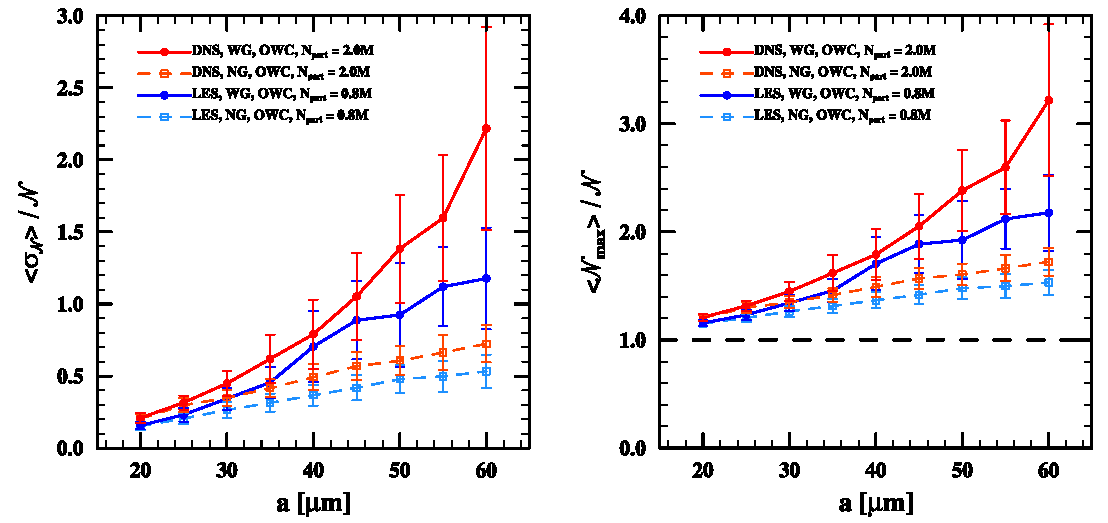
\includegraphics[width=13.5cm]{img/plots/3-4c-pfpowc.pdf}
\caption{
Time-averaged standard deviation, $\langle \sigma(\mathcal{N}) \rangle$ (left), and maximal number of particles in~subdomains, $\langle \mathcal{N}_{\max} \rangle$ (right), for OWC simulations with and without gravity (DNS and LES).
Values are normalised by the average number of particles per subdomain.
}
\label{fig:pfpowc}
\end{figure}

As before, when these statistics are compared with respective plots of average wallclock times per step (see Figure \ref{fig:pfsowc}), it can be seen that particle distribution plays a major role in determining overall computational performance of a simulation.
It is a more complex task to explain why the nonunifirmity of distribution is influenced to such a degree by droplet radii and the presence of gravity.
Most notably, the supposed relationship of the particle distribution statistics and the RDF (see Figure \ref{fig:owcrdfrrv}) cannot be easily identified.
It is especially striking for simulations without gravity where distinctive trend of the RDF, with a clear peak at $a \sim 35$~$\upmu\text{m}$, is nowhere to be seen.
It is possible that such dependence manifests in fluctuations of $\langle \mathcal{N}_{\max} \rangle / \mathcal{N}$ but is dwarfed by other more dominant factors.
  
Before, it was suggested that the substantial increase in variance of particle distribution with growing radii of droplets may be explained by specific behaviour of particle clusters under the influence of gravity.
Settling droplets with high inertia tend to concentrate in column-like structures along the direction of gravity vector.
In this implementation, $\mathbf{g}$ is assumed to be aligned with subdomain ``pencils''.
Such choice was made to limit the number of particles that cross subdomain boundaries \parencite{Ayala2014}.
This alignment, however, may induce unwanted concentration of particles in few subdomains that contain such clusters.

\begin{figure}[!htbp]
\centering
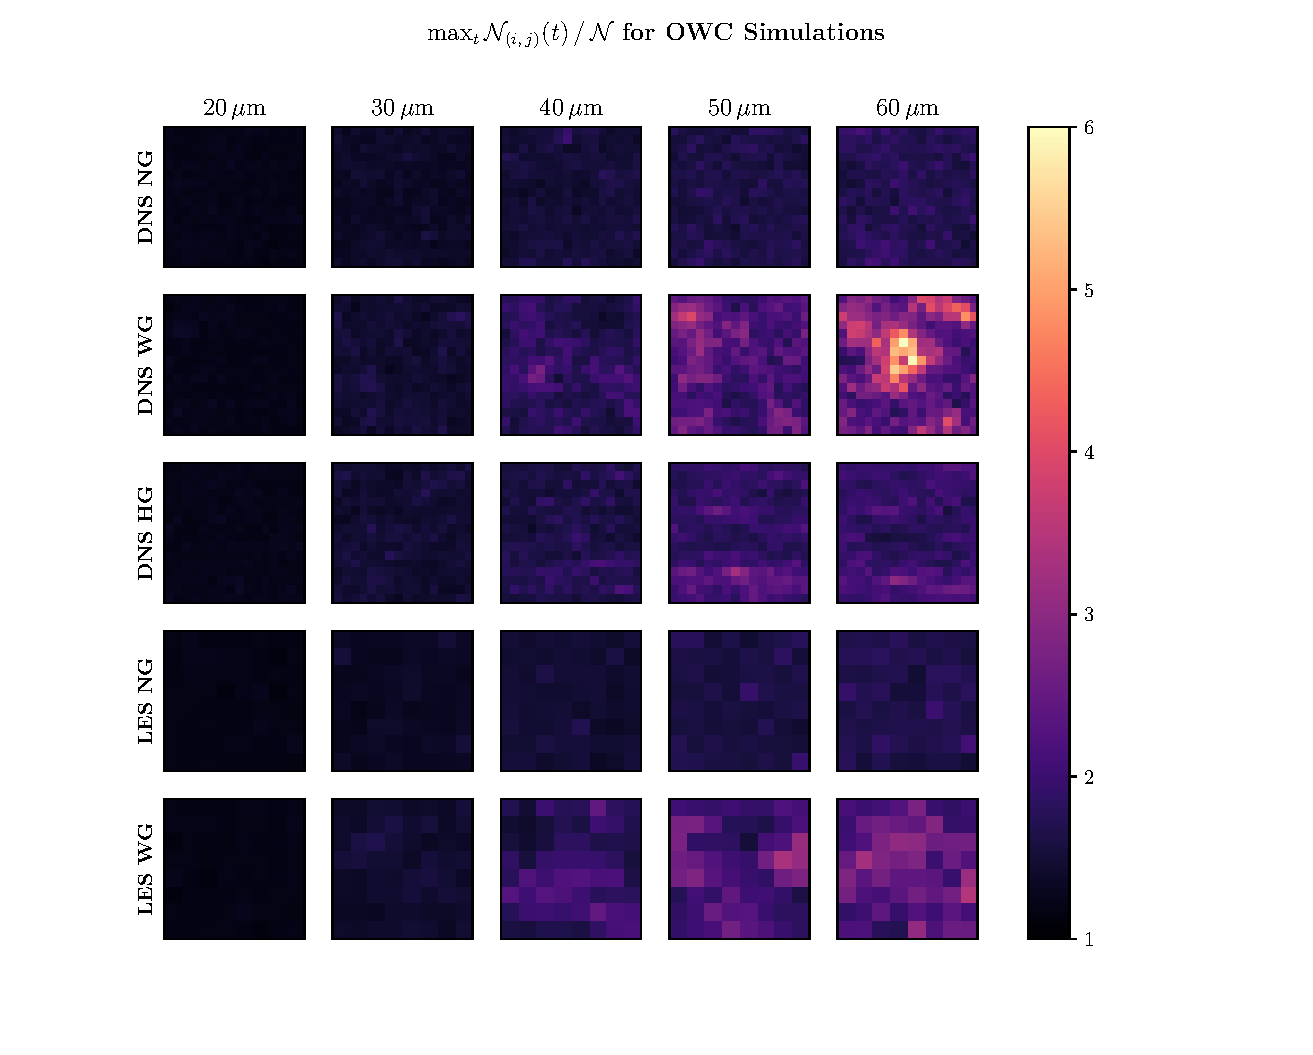
\includegraphics[width=17cm]{img/plots/3-4f-pfpgridowcmax.pdf}
\caption{
Maximum number of particles for every subdomain taken over the entire simulation run for OWC simulations with droplets of different radii.
Results are included for both DNS and~LES: NG -- without gravity, WG -- with gravity; HG -- with ``horizontal'' gravity, i.e. that is pointing perpendicular to the domain boundaries.
Values are normalised by the average number of particles per subdomain.
}
\label{fig:pfpgridowcmax}
\end{figure}

In order to qualitatively verify such claim, respective particle distribution statistics were calculated separately for every subdomain with respect to time.
In particular, values of $\max_{t} \mathcal{N}_{(i,\,j)}(t)$ were obtained by finding the maximum number of particles for any given subdomain $(i,\,j)$ across all considered time steps $t$.
The values of $\sigma_{t} (\mathcal{N}_{(i,\,j)}(t))$ were calculated accordingly by taking standard deviations of particle counts in time.
These statistics were plotted on the 2D grids that are consistent with the topology of subdomains in the system.

\begin{figure}[!h]
\centering
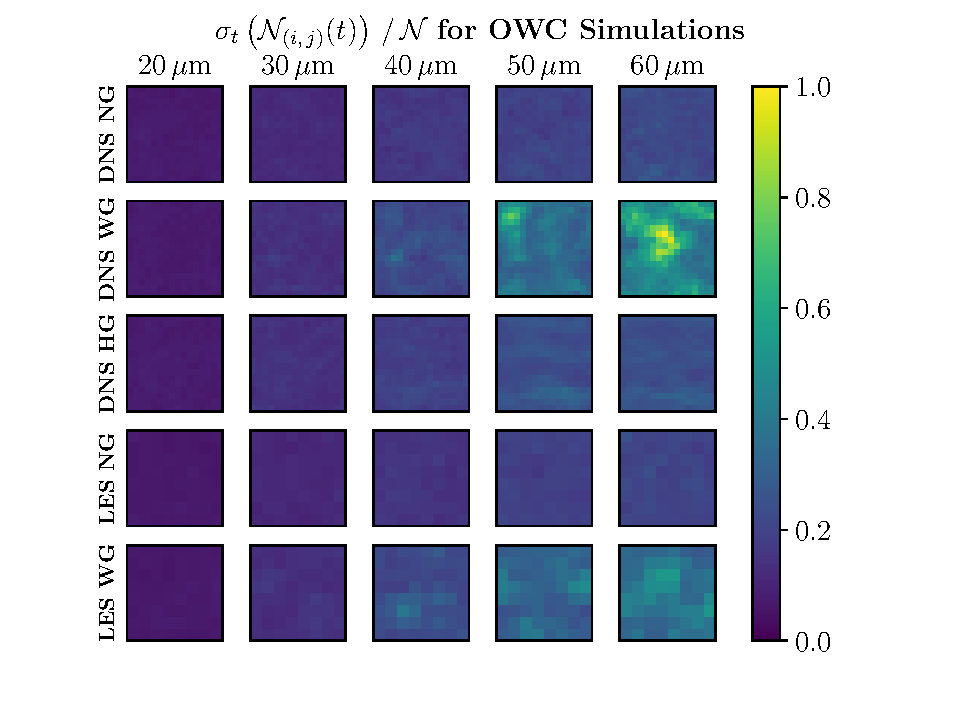
\includegraphics[width=13.5cm]{img/plots/3-4g-pfpgridowcstd.pdf}
\caption{
Standard deviation of particle counts for every subdomain taken over the entire simulation run for OWC simulations with droplets of different radii.
Consistent with Figure \ref{fig:pfpgridowcstd}.
}
\label{fig:pfpgridowcstd}
\end{figure}

The results for a regime of OWC simulations are shown in Figures \ref{fig:pfpgridowcmax} and \ref{fig:pfpgridowcstd}.
They clearly show that indeed both maxima and standard deviations taken over time for large settling droplets tend to concentrate in one or few regions of the domain.
For DNS with gravity such maxima reach values of $6 \mathcal{N}$ (for $a = 60$~$\upmu\text{m}$), indicating that some processes become severely overloaded by particles which consequently explains steep increase in average step times.
Note, however, that corresponding values of $\langle \mathcal{N}_{\max} \rangle / \mathcal{N}$ and their uncertainties show that such extreme concentrations are not regularly achieved.

When gravity is not considered, no distinct regions of considerably higher particle concentration are discernible.
Upon closer inspection some nonuniformities may be noticed for~heavier non-settling droplets but they are relatively mild and evenly spaced out.
This is due to the fact that without effects of gravity particle clusters have more isotropic structure and distribution.
Still, even without gravity we see steady increase in maxima and standard deviations of particle counts in subdomains when the droplet radii become larger.
This monotonic increase is inconsistent with the drop in the RDF for $a > 50$~$\upmu\text{m}$, hence it may be concluded that, at least in this case, properties of particle distribution in subdomains follow from clustering phenomena on larger spatial scales that are not captured by the RDF at contact distance. 

\begin{figure}[!h]
\centering
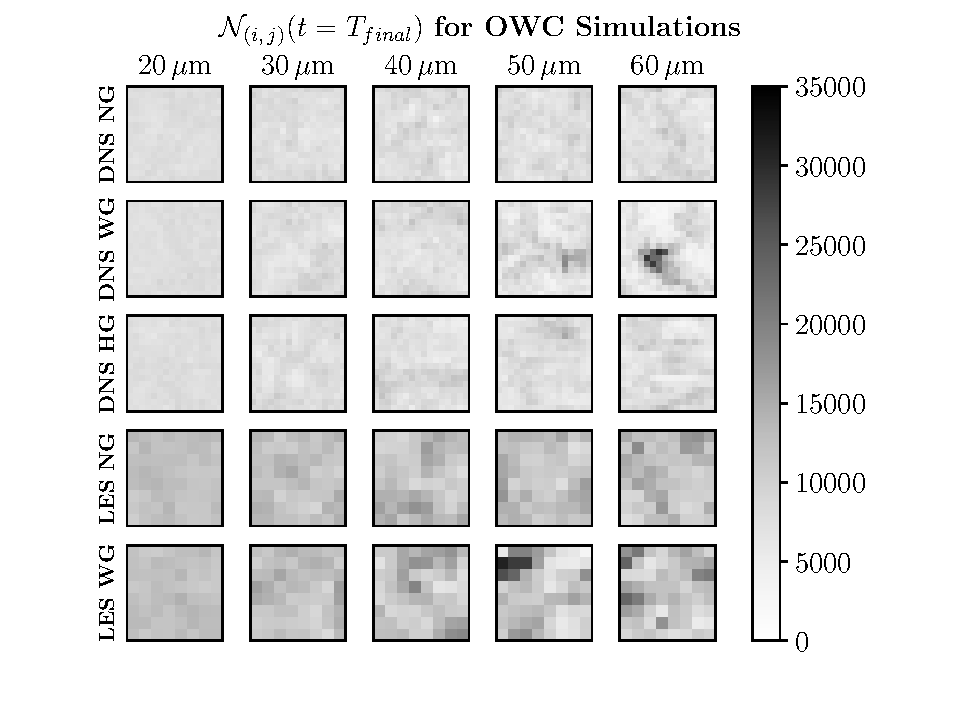
\includegraphics[width=13.5cm]{img/plots/3-4h-pfpgridowclast.pdf}
\caption{
Particle counts for every subdomain taken from the last processed time step for OWC simulations with droplets of different radii.
Average number of particles per subdomain are: $7 812.5$ for DNS, $12 500$ for LES.
Consistent with Figure \ref{fig:pfpgridowcstd}.
}
\label{fig:pfpgridowclast}
\end{figure}

For more illustration, Figure \ref{fig:pfpgridowclast} shows actual particle counts collected at the last processed time step of respective OWC simulations.
This provides a snapshot of the system in one particular point in time without any averaging.  
The particle distributions for simulations without exhibit some regions where particle concentrations are elevated at given point in time, but in the long run they average out to relatively uniform distribution of attained maxima. 
More importantly, in the case of heavy settling droplets, the region of high particle concentration ($\sim 4 \mathcal{N}$) is present, although its location in not precisely aligned with a single region of highest maxima or standard deviation (see Figures \ref{fig:pfpgridowcmax} and \ref{fig:pfpgridowcstd}).
In fact, when particle counts are analysed in time, such clusters are moving across the domain.
Still, they statistically tend to occupy one region that is characterised by relatively high average maxima and standard deviations.
Such behaviour in time may be directly witnessed for droplets with radius $60$~$\upmu\text{m}$ in animation available here: \url{https://github.com/xann16/talks/blob/master/msc-thesis/extras/pfp-owc-anim.gif}.
These visualisations provide coarse, yet insightful perspective of the dynamics of the disperse phase influenced by background turbulence.

\medskip

To further analyse the influence of gravity on the computational performance of simulations, a small side experiment was performed.
The same set of OWC simulations (DNS only) was performed with the direction of gravity changed to be perpendicular to the subdomain boundaries.
Such change should lead to the increased computational effort devoted to the relocation of particles between subbdomains, as they have relatively higher velocities in the direction of gravity.
On the other hand, any anisotropic clusters of particles aligned with the direction gravity should be spread across several subdomains and not contained within relatively few ``pencils''.
In light of previous analyses it is conjectured that performance gains from the latter effect may outweigh additional costs associated with the former.

\begin{figure}[h]
\centering
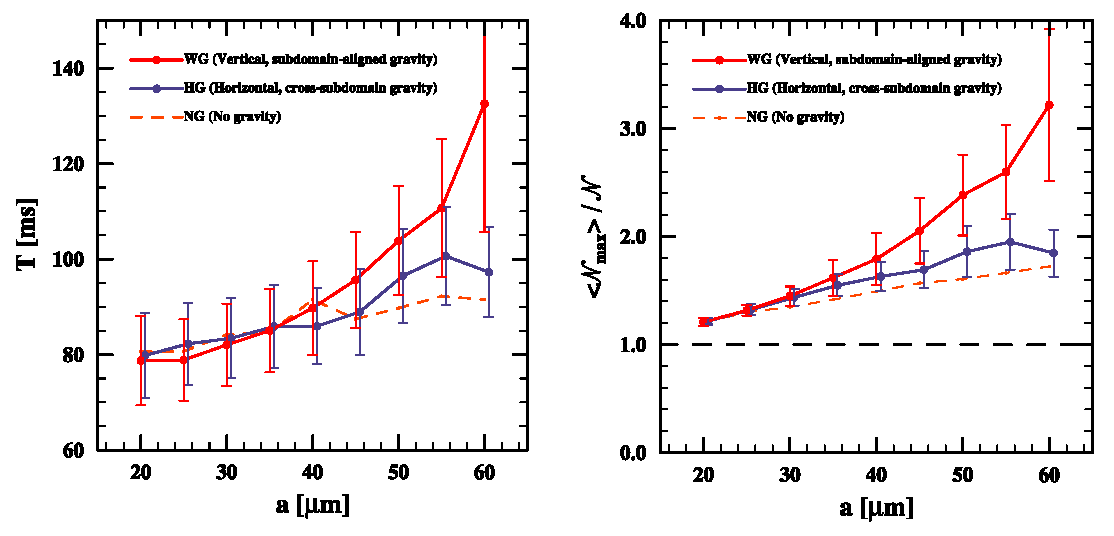
\includegraphics[width=13.5cm]{img/plots/3-4d-howcperf.pdf}
\caption{
Time-averaged wallclock times per step, $T$ (left), and normalised maximal number of~particles in subdomains, $(\langle \mathcal{N}_{\max} \rangle / \mathcal{N})$ (right) for DNS simulations under one-way momentum coupling (OWC) with different directions of gravity with respect to domain decomposition.
For comparison results for simulations without gravity are shown with dashed line. 
}
\label{fig:howcperf}
\end{figure}

Figure \ref{fig:howcperf} (left) shows results of performance measurements for OWC DNS with gravity pointing in two directions: ``vertical'' (standard, parallel to boundaries between subdomains) and ``horizontal'' (perpendicular to subdomain boundaries).
The average wallclock times per step indicate that assumption introduced above is correct.
Although uncertainties associated with time measurements are relatively high and caution is advised, the results for heaviest droplets ($a = 60$~$\upmu\text{m}$) indicate unequivocal and considerable reduction of the simulation time.
In general, the values of $T$ show a pattern that was expected.
For smaller droplets ($a < 35$~$\upmu\text{m}$) changing the direction of gravity to ``horizontal'' leads to increase in $T$, as column-like particle clusters are not as pronounced to provide any performance gain or even cancel out additional effort spent on particle relocation.   

On the other hand, for particles with radius $40$~$\upmu\text{m}$ and larger the positive effects of~the~rotated direction of gravity become appreciable.
This is further enforced by respective $\langle \mathcal{N}_{\max} \rangle / \mathcal{N}$ (Figure \ref{fig:howcperf}, right).
The average maxima of particle counts across subdomains are visibly reduced throughout considered range of droplet radii.
For the smallest droplets ($a < 30$~$\upmu\text{m}$) the difference is negligible, but with larger radii the change in favour of the ``horizontal'' gravity only increases.
In extreme case, for $a = 60$~$\upmu\text{m}$ the reduction in $\langle \mathcal{N}_{\max} \rangle$ is close to $45 \%$.
Note, that Figures \ref{fig:pfpgridowcmax}, \ref{fig:pfpgridowcstd} and \ref{fig:pfpgridowclast} also contain plots for simulations conducted with ``horizontal'' gravity (labelled ``DNS HG'').
They show considerably smaller values of measured parameters than in standard simulations with gravity.
Moreover, elongated horizontal features are clearly visible and they correspond to the gravity-aligned column-like clusters of particles that were rotated $90^{\circ}$ and now span across entire rows of subdomains.
This leads to more even distribution of particles between subdomains and consequently reduced simulation times.

\begin{figure}[!h]
\centering
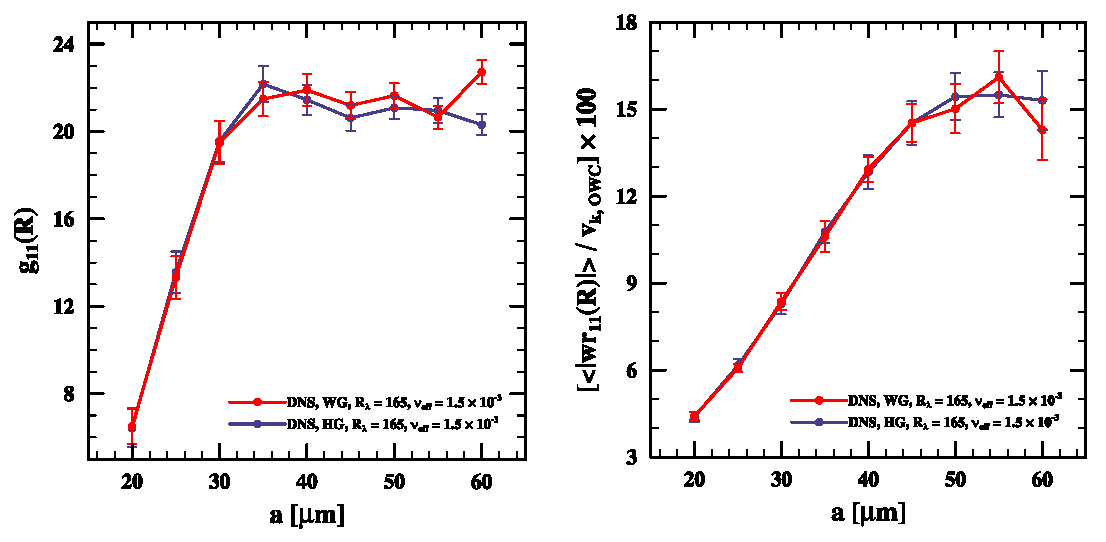
\includegraphics[width=13.5cm]{img/plots/3-4e-howcrdfrrv.pdf}
\caption{
The values of the radial distribution function (RDF, left) and the radial relative velocity (RRV, right) at contact distance for simulations with one-way momentum coupling.
Results include data from DNS simulations with different directions of gravity vector with respect to domain decomposition.
}
\label{fig:howcrdfrrv}
\end{figure}

These results further validate previous explanation of mechanisms that lead to increased average wallclock times per step for simulations with gravity when droplet radii become larger.
Moreover, they establish a simple alternative that can lead to significant gains in performance and require minimal effort in code development.
In theory, changing the direction of gravity should result in no appreciable difference in the physics of modelled system, thus obtained statistics should be independent of any specific direction chosen.
This is verified for the kinematic statistics of particles in Figure \ref{fig:howcrdfrrv}.
Both approaches produce results that are, for the most part, well within the margin of statistical uncertainty.
The only significant discrepancy is for droplets of radii $60$~$\upmu\text{m}$, especially in the case of the RDF.
The reason for this difference, however, does not lie in the implementation of the numerical model, but in the physics of the problem.
Settling of high inertia particles leads to formation of elongated clusters that can remain stable for a long time.
Hence, RDF reveals a stronger dependence on initial conditions or, in other words, on a given realisation.
In general, the use of alternative direction of gravity in the pseudo-spectral solver requires broader examination in order to fully demonstrate that it guarantees consistency of physical results and provides reproducible performance gains (within certain bounds of applicability, i.e. for heavy settling particles).

\begin{figure}[!h]
\centering
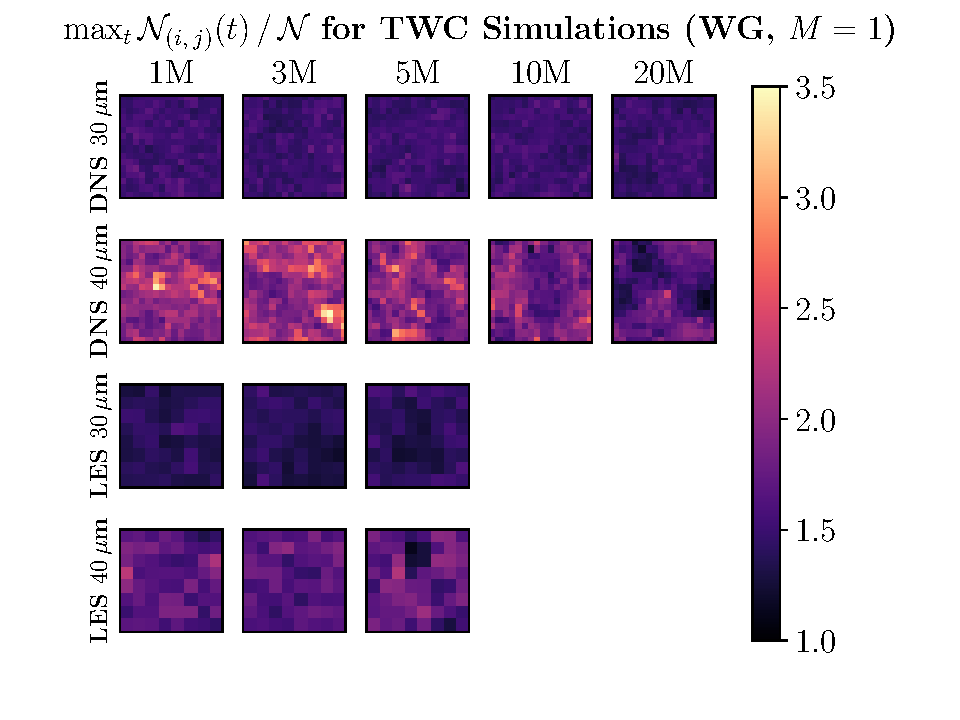
\includegraphics[width=10cm]{img/plots/3-4i-pfpgridtwcmax.pdf}
\caption{
Maximum number of particles for every subdomain taken over the entire simulation run for TWC simulations with gravity and radii $30$, $40$~$\upmu\text{m}$.
All simulations were conducted without superparticle parameterisation ($M=1$). 
Values are normalised by the average number of particles per subdomain.
Consistent with Figure \ref{fig:pfpgridowcmax}.
}
\label{fig:pfpgridtwcmax}
\end{figure}


\medskip

In addition, Figures \ref{fig:pfpgridtwcmax} and \ref{fig:pfpgridrdfstd} are presented as an additional illustration of the particle distribution statistics for TWC simulations.
Firstly, note that the range of the particle count maxima attained by TWC simulations are considerably smaller than those under one-way momentum coupling (see Figure \ref{fig:pfpgridowcmax}).
This is due to smaller droplet radii (with radii $30$,~$40$~$\upmu\text{m}$).
For $a = 30$~$\upmu\text{m}$ almost no appreciable difference in plots can be noticed when $N_{\text{part}}$ increases.
This is consistent with previously shown statistics (Figure \ref{fig:pfptwc}) and respective RDF (Figure \ref{fig:twcrdfext}).
On the other hand, for $a = 30$~$\upmu\text{m}$ we observe a range of interesting patterns that are being suppressed with the increase of the mass loading.
These coarse-grained and discrete images that compress some information on the state of the disperse phase may be compared with more detailed plots presented in \textcite[Figure 9bc]{Rosa2020} with precise positions of droplets (from a limited horizontal slice of the domain).
Interestingly, when both pictures are compared for droplets with $a = 30$~$\upmu\text{m}$ and $a = 40$~$\upmu\text{m}$, the latter tend to arrange in larger-scale clusters.
That is also reflected in Figure \ref{fig:pfpgridtwcmax}.
Note that for TWC simulations with droplets of radii $40$~$\upmu\text{m}$ similar animations were prepared as for OWC, and are available here: \url{https://github.com/xann16/talks/blob/master/msc-thesis/extras/pfp-twc-anim.gif}.

\begin{figure}[h]
\centering
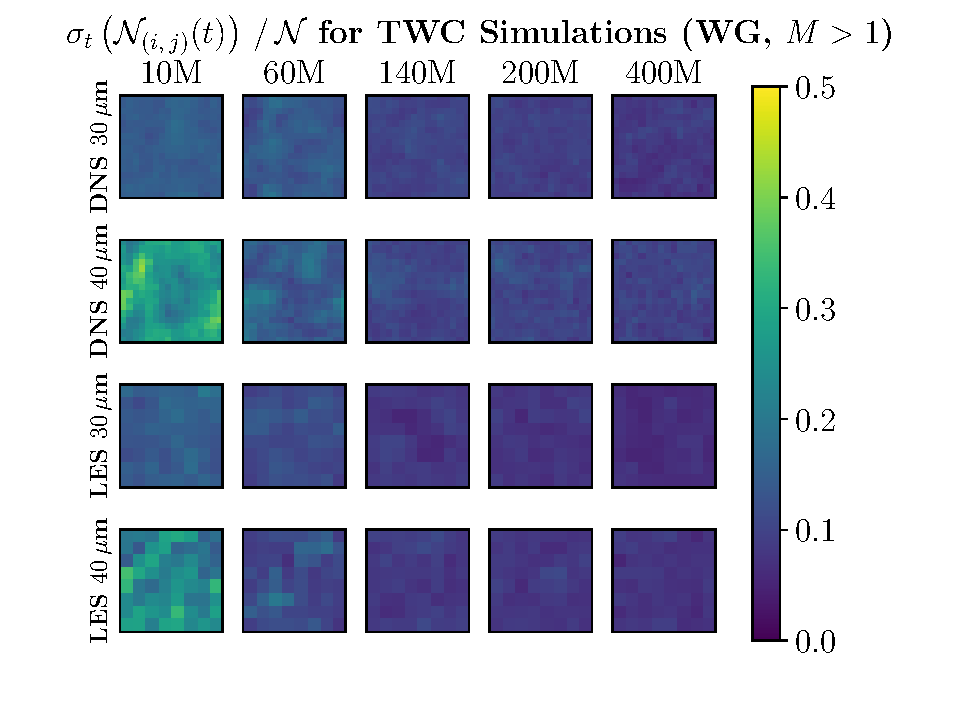
\includegraphics[width=10cm]{img/plots/3-4j-pfpgridrdfstd.pdf}
\caption{
Standard deviation of particle counts for every subdomain taken over the entire simulation run for TWC simulations with gravity and radii $30$, $40$~$\upmu\text{m}$.
All simulations were conducted with superparticle parameterisation ($M>1$). 
Values are normalised by the average number of particles per subdomain.
Consistent with Figure \ref{fig:pfpgridowcstd}.
}
\label{fig:pfpgridrdfstd}
\end{figure}





\chapter*{Conclusions}
\addcontentsline{toc}{chapter}{\numberline{}Conclusions}
\label{ch:end}

The main goal of this thesis was the comparison of DNS and LES methods in terms of physical fidelity and computational performance, especially when two-way momentum coupling between fluid and particles is considered.
For that purpose, a substantial amount of data was obtained from over 500 simulations of varying complexity and computational cost.
Significant part of these involved a well-established DNS method, and serve as further validation of previously published results, as well as a way of confirming the correctness of employed solver and other software used in data processing.
Much more important, however, were simulations that utilised LES method with two-way momentum coupling, as they provide entirely novel insight into possibilities and challenges of modelling particle-laden flows with homogeneous isotropic turbulence.
The usage of deterministic forcing with LES simulations is also a new contribution in that field, including motivated by that fact short side-study of the influence of spectral viscosity model parameter $C_K$ on turbulence spectra and statistics.
Another important aspect of this study is the broad analysis of the computational costs of such simulations, including in-depth code profiling and unique attempt to tie code performance to the distribution of~particles among subdomains.

The comparison of turbulent flow statistics and collisional particle statistics shows that LES may be considered as a promising alternative to DNS and a way to simulate systems characterised by higher Reynolds numbers, closer to those of real-life atmospheric air turbulence.
Due to used parameterisation of small-scale turbulence, however, some level of inaccuracy has to be expected.
In case of one-way momentum coupling these effects were already studied, and are confirmed here, as they are also applicable to some degree under two-way momentum coupling.
In particular, the underestimation of the radial distribution function and overestimation of radial relative velocities are observed with two-way coupling, although such discrepancies diminish with the increase of particle mass loading.
Interestingly, these effects tend to cancel each other when collision kernel is considered, especially for particles of radius of $30$~$\upmu\text{m}$ ($St \approx 0.5$).
In general, LES results tend to follow those of DNS more closely, both quantitatively and in terms of relative trends, for settling particles.

There are, however, some circumstances where filtering of small scales in TWC LES leads to accumulation of inaccuracies.
The most striking example are systems with large amounts of relatively small settling particles.
Such particles tend to strongly modulate small-scale turbulence, which is filtered in LES, thus leading to significant discrepancies in kinematic particle statistics and collision kernel.
The main issue here seems to be that subgrid-scale model used in this study is agnostic to the influence of particles on the fluid, hence any turbulence modulation that affects predominantly small scales has no effect.
This limits indirect influences that neighbouring particles exert on each other by affecting background flow.
Thus, it is a~viable direction to conduct similar studies as this one but focusing on different subgrid-scale models that may alleviate some of aforementioned drawbacks.
The~far-reaching goal here, would be the development of the ''hybrid'' model that could use the information about the~state of particles to adjust its parameterisation of small scale turbulence.

The analysis of computational performance have shown major difference in bottlenecks that need to be addressed for DNS and LES.
The implementation of pseudo-spectral solver that was used in this study was developed with DNS in mind, therefore its parallelisation strategy is focused on evenly splitting considerable burden associated with the integration of the fluid flow.
For LES, however, with the reduction of grid size comes the shift in priorities, as calculations associated with particles become the dominating contributor to the computational complexity of the entire simulation.
For that reason, the current adaptation of the solver to incorporate subgrid-scale model was found to be non viable for systems with the number of individually tracked particles that exceeds 5 million.
In general, the main cause of rapidly increasing simulation times with larger number of particles is the postprocessing stage.
These tasks, where particle-pair statistics are computed, exhibit quadratic complexity with respect to the number of particles assigned to any given subdomain.
Moreover, it requires synchronisation of all executing processes at the end of the stage which ties the time of execution of the entire iteration to the computational cost of a single process with maximal workload in terms of particle count for any given time step.
This makes the particle distribution across computational subdomains and the degree of its nonuniformity an important factor to the overall performance of simulations.
Moreover, it was found to be the reason for the growth of computational costs of simulations when droplet radii increases, especially for settling particles.
To alleviate some problems in that context the use of ``horizontal'' (i.e. perpendicular to the boundaries between subdomains in 2D decomposition) direction of gravity was proposed, and its positive impact on making the particle distribution in parallel processes more uniform was demonstrated.

Even though LES has theoretical advantages over DNS in terms of performance, to fully embrace that potential for simulations with larger mass loadings an alternative paralellisation strategy needs to be developed.
The key issue here is splitting the computations associated with particles between larger number of processes.
The simplest solution would be to consider several independent sets of particles, as was proposed by \textcite{Ayala2014}, or further subdivide the computational domain along physical boundaries, e.g. using 3D decomposition only for particle-related workload.
Both of these solutions have its own issues and need to be thoroughly examined to obtain expected computational performance and scaling.
In general, for both DNS and LES, the stage devoted to the postprocessing of particle statistics was found to be one of the main bottlenecks.
The core of its calculations is the cell-index method coupled with the concept of linked lists proposed by \textcite{Allen1987}.
This approach is well-established in studies like this, but may be the prime candidate for optimisation efforts that would prove relevant for the efficiency of numerical experiments focused on collision statistics.
Also, since it was established that the variance of particle distribution in the domain may be an important factor when simulating particle-laden turbulent flows, a degree of adaptivity may be considered.
For example, certain data structures specific to computer graphics and point cloud processing, such as quadtrees, octrees, or K-d trees, may be used to enhance currently used methods.
Such adaptive solutions can be used exclusively to keep track of the neighbouring particles for the purpose of the postprocessing stage, but also can be fully developed into an adaptive decomposition scheme to evenly spread particle workload among available parallel processes. 




\appendix
\chapter{Pseudo-Spectral Method in Detail}
\label{app:psm}

This section provides more detailed description of the pseudo-spectral method used in present study to simulate homogeneous isotropic turbulence. 
This method is convenient for numerical integration of time-dependent, incompressible Navier-Stokes equations on a regular three-dimensional mesh.
Originally, it was introduced in \textcite{Orszag1972} and later applied and expanded upon in other publications, such as \textcite{Rogallo1981,Eswaran1988,Pope2000,Peng2009}.

This section provides more detailed description of the pseudo-spectral method used in present study to simulate homogeneous isotropic turbulence. This method is convenient for numerical integration of time-dependent, incompressible Navier-Stokes equations on a regular three-dimensional mesh.
 


\subsubsection{Domain Discretisation in Physical and Spectral Space}

We assume that our domain is a cube with side length of $\mathcal{L}$ and periodic boundary conditions are applied in each spatial direction.
The dynamic quantities are spatially discretised using uniform rectangular grid with $N$ nodes per side, or $N^3$ nodes in total, with grid spacing $\mathcal{L} / N$.
Additionally, we assume that $N$ is even (preferably, a power of $2$, to work well with FFT), and 
$$ \mathcal{L} = \mathcal{L}_x = \mathcal{L}_y = \mathcal{L}_z = 2 \pi \, .$$

Points in physical space are given at $N^{3}$ nodes as $\mathbf{x} = (n_1 \Delta x, n_2 \Delta y, n_3 \Delta z)$, where $n_1, n_2, n_3 \in \{ 0, \ldots, N - 1 \}$ and $\Delta x = \Delta y = \Delta z = N / (2 \pi)$.
In spectral space, we consider $N^3$ discrete wavenumbers $\mathbf{k} = (k_1, k_2, k_3)$, that are given by $(m_1 k_0, m_2 k_0, m_3 k_0)$, where $m_1, m_2, m_3 \in \{ -(N / 2) + 1 , \ldots, N / 2 \}$, and the lowest wavenumber, $k_0$, is equal to $(2 \pi) / \mathcal{L}$, which under adopted assumption that $\mathcal{L} = 2 \pi$ reduces to $1$, therefore discrete wavenumbers are integers equal to their respective grid indices $m_1$, $m_2$ and $m_3$.
Limited, finite number of modes are resolved in spectral space, with maximal wavenumber set to $k_{\max} = \left\lfloor \frac{N - 3}{2} \right\rfloor$ (in~particular, for $N=256$, we have $k_{\max} = 126$).


Furthermore, we consider fluid velocity field $\mathbf{U}(\mathbf{x}, t)$ defined at discrete grid nodes.
Then, its corresponding Fourier coefficients in spectral space are calculated using the \emph{discrete Fourier transform} in three dimensions:
\begin{align*}
\mathbf{\hat{U}}(\mathbf{k}, t) &= \frac{1}{N^3} \sum_{\mathbf{x}} \mathbf{U}(\mathbf{x}, t) \exp(-i \mathbf{k} \cdot \mathbf{x}) \\
                                &= \frac{1}{N^3} \sum_{n_1 = 0}^{N-1} \sum_{n_2 = 0}^{N-1} \sum_{n_3 = 0}^{N-1} \mathbf{U} ((n_1 \Delta x, n_2 \Delta y, n_3 \Delta z), t) \exp(- \frac{2 \pi i}{N}(n_1 k_1 + n_2 k_2 + n_3 k_3)) \, ,
\end{align*}
where summation is defined over all nodes in physical space.
Conversely, to obtain physical velocity back from the Fourier coefficients, we apply the \emph{inverse discrete Fourier transform}, expressed as follows:
\begin{align*}
\mathbf{U}(\mathbf{x}, t) &= \sum_{\mathbf{k}} \mathbf{\hat{U}} (\mathbf{k}, t) \exp(i \mathbf{k} \cdot \mathbf{x}) \\
                          &= \sum_{k_1 = - \frac{N}{2} + 1}^{\frac{N}{2}} \sum_{k_2 = - \frac{N}{2} + 1}^{\frac{N}{2}} \sum_{k_3 = - \frac{N}{2} + 1}^{\frac{N}{2}} \mathbf{\hat{U}}((k_1, k_2, k_3), t) \exp \left( - \frac{2 \pi i}{N}(n_1 k_1 + n_2 k_2 + n_3 k_3) \right) \, .
\end{align*}

Since periodic boundary condition are imposed, we have
$$ \mathbf{U}(\mathbf{x} + 2 \ell \pi, t) = \mathbf{U}(\mathbf{x}, t)$$
for any considered $\mathbf{x}$ and $t$, as well as any $\ell \in \mathbb{Z}$.
In addition, we enforce velocity field to be zero-mean, i.e.:
$$ \mathbf{\hat{U}}(\mathbf{0}, t) = 0$$
for all $t$.

\subsubsection{Navier-Stokes Equations in Physical and Spectral Spaces}

In physical (position) space \emph{Navier-Stokes equations} include both \emph{continuity equation}:
\begin{equation}
\label{eqn:cont}
\nabla \cdot \mathbf{U} = 0 \, ,
\end{equation}
and \emph{momentum equation}:
\begin{equation}
\label{eqn:mom}
\frac{\partial}{\partial t} \mathbf{U} = \mathbf{U} \times \boldsymbol{\omega} - \nabla \left( \frac{P}{\rho} + \frac{U^2}{2} \right) + \nu \nabla^2 \mathbf{U} + \mathbf{f} \, ,
\end{equation}
where $\mathbf{U} := \mathbf{U}(\mathbf{x}, t)$ is a fluid velocity field (note: $U^2 = \mathbf{U} \cdot \mathbf{U}$), $ \boldsymbol{\omega} := \boldsymbol{\omega}(\mathbf{x}, t) = \nabla \times \mathbf{U}(\mathbf{x}, t) $ is its vorticity, $\mathbf{f} := \mathbf{f}(\mathbf{x}, t)$ is a large scale force (acting on large turbulent scales, i.e. affecting only low wavenumbers), $P$ is pressure, $\rho$ is constant density of a fluid, and $\nu$ -- its kinematic viscosity.

On the right hand side of equation (\ref{eqn:mom}) first two terms represent two parts of a \emph{nonlinear term}. They are obtained using following identity:
$$ - \mathbf{U} \cdot \nabla \mathbf{U} = \mathbf{U} \times \boldsymbol{\omega} - \nabla \left( \frac{U^2}{2} \right) \, . $$
For convenience, we will use following notation for these terms:
$$ \mathbf{N_1} := \mathbf{U} \times \boldsymbol{\omega} $$
and, for the scalar part, the gradient of which is the second term, we define:
$$ N_2 := \frac{P}{\rho} + \frac{U^2}{2} \, . $$
As for remaining terms, third one expresses effects of kinematic viscosity (diffusive term), while the last one effects of large scale forces acting on the fluid.

When we transition to the \emph{spectral space} (also referred to as the \emph{wavenumber} or \emph{Fourier} space), the momentum equation (\ref{eqn:mom}) becomes:
\begin{equation}
\label{eqn:mom-spec}
\frac{\partial}{\partial t} \mathbf{\hat{U}} = \mathbf{\hat{N}_1} - i \mathbf{k} \hat{N}_2 - \nu k^2 \mathbf{\hat{u}} + \mathbf{\hat{f}} \, ,
\end{equation}
where $\mathbf{\hat{U}} := \mathbf{\hat{U}}(\mathbf{k}, t)$ is a fluid velocity amplitude in spectral space, $\mathbf{\hat{f}} := \mathbf{\hat{f}}(\mathbf{k}, t)$ is a large scale force that is acting only on low wavenumbers, $\mathbf{\hat{N}_1}$ and $\hat{N}_2$ represent terms defined above, but expressed in the spectral space.
We observe typical for Fourier transform elimination of spatial derivatives, that reduces our equation to the system of ODEs of time variable $t$. 

\subsubsection{Nonlinear Term in Spectral Space}

First, we may observe that since forcing term $\mathbf{f}$ is incompressible "by design", it satisfies the reduced continuity equation, i.e. that
$$ \nabla \cdot \mathbf{f} = \mathbf{0} \, , $$
or in spectral space:
$$ i \mathbf{k} \cdot \mathbf{\hat{f}} = \mathbf{0} \, . $$
Thus, continuity equation (\ref{eqn:cont}) implies that, in particular:
$$ \nabla \cdot \mathbf{N}_1 - \nabla^2 N_2 = \mathbf{0} \, . $$
Therefore, in spectral space:
$$ i \mathbf{k} \cdot \mathbf{\hat{N}_1} - (-k^2) \hat{N}_2 = \mathbf{0} \, , $$
or, equivalently:
$$ \hat{N}_2 = - \frac{i \mathbf{k} \cdot \mathbf{\hat{N}_1} }{k^2} \,. $$
This means that the second (scalar) part of the nonlinear term can be easily obtained from the first (vector) part of the nonlinear term in the spectral space.
In conclusion, the full nonlinear term, may be expressed in spectral space as follows:
\begin{equation}
\label{eqn:nonlin-spec}
\mathbf{\hat{N}_1} - i \mathbf{k} \hat{N}_2 = \mathbf{P}_{ij}( \mathbf{k} ) \left[ \mathbf{\hat{N}_1} \right]_{j} \, ,
\end{equation}
assuming summation notation, where $\mathbf{P}_{ij}$ is a projection tensor defined as:
\begin{equation}
\label{eqn:proj-tensor}
\mathbf{P}_{ij}( \mathbf{k} ) = \mathbf{\delta}_{ij} - \frac{k_{i} k_{j}}{k^2} .
\end{equation}
In equation \ref{eqn:nonlin-spec}, the vector part of nonlinear term is projected onto a plane normal to $\mathbf{k}$.
This way, by rearranging terms, we may express $\hat{N}_2$ in terms of $\mathbf{\hat{N}_1}$, thus eliminating the dependence on pressure (that itself depends entirely on the velocity field and its derivatives) in our equation by using the continuity equation as a constraint. 
This relation, in a discretised form, will be used later to simplify process of numerical integration of the momentum equation in spectral space.


\subsubsection{Representation of Discrete Grid in Spectral Space}

The following method is used to represent wavevector $\mathbf{k}$, as well as, $k^2$:
$$
\mathbf{k} =
\begin{bmatrix}
k_1 \\ k_2 \\ k_3
\end{bmatrix}
=
\begin{bmatrix}
\text{fac1}(1 \rightarrow N + 2) \\ \text{fac2}(1 \rightarrow N) \\ \text{fac3}(1 \rightarrow N)
\end{bmatrix} ,
\quad
k^2 =
\begin{bmatrix}
k_1^{\; 2} \\ k_2^{\; 2} \\ k_3^{\; 2}
\end{bmatrix}
=
\begin{bmatrix}
\text{fsq1}(1 \rightarrow N + 2) \\ \text{fsq2}(1 \rightarrow N) \\ \text{fsq3}(1 \rightarrow N)
\end{bmatrix}
\, .
$$
In particular, for first dimension we have the following indices:
$$ \text{fac1}(1 \rightarrow N + 2) = (0, 0, 1, 1, 2, 2, \ldots, N/2 - 1, N/2 - 1, N/2, N/2)  $$
where alternating elements represent real and imaginary parts, respectively, of complex values.
We may save half of the spectral space by representing only values for non-negative indices, since negative ones may be retrieved from symmetry by complex conjugation, as
$$ \mathbf{\hat{U}}(- \mathbf{k}, t) = \mathbf{\hat{U}}^* (\mathbf{k}, t) \, . $$
For remaining dimensions, we use the following
\begin{align*}
\text{fac2}(1 \rightarrow N) &= (0, 1, 2, \ldots, N/2 - 1, N/2, -(N/2 -1), -(N/2 -2), \ldots, -2, -1) \\
\text{fac3}(1 \rightarrow N) &= (0, 1, 2, \ldots, N/2 - 1, N/2, -(N/2 -1), -(N/2 -2), \ldots, -2, -1) \, .
\end{align*}

\subsubsection{General Solution Procedure}

In broad terms, the pseudo-spectral method is characterised by using a mixture of computations performed in both physical and spectral spaces, depending on where it is more convenient or efficient. 
The spatial derivatives are evaluated in the wavenumber space.
Then, to facilitate computation, the cross products are calculated in the physical space.

Specifically, to describe one entire step of evolution in time of the model, we assume that the problem has been already solved for the former time steps up to $n$, i.e.  following velocity fields are known
$$ \mathbf{\hat{U}}(\mathbf{k}, \Delta t) , \, \mathbf{\hat{U}}(\mathbf{k}, 2 \Delta t) , \, \ldots , \, \mathbf{\hat{U}}(\mathbf{k}, n \Delta t) \, .  $$
The further procedure to solve for $\mathbf{\hat{U}}(\mathbf{k}, (n+1) \Delta t)$ consists of four steps:
\begin{enumerate}
\item The velocity field $\mathbf{U}$ in physical space is obtained from the Fourier coefficients in the spectral space by applying inverse fast Fourier transform, i.e.:
\begin{equation}
\mathbf{\hat{U}}(\mathbf{k}, n \Delta t) \xrightarrow{\; \text{FFT}^{-1}} \, \mathbf{U}(\mathbf{x}, n \Delta t) \, .
\label{eqn:psproc-1}
\end{equation}
\item We calculate vorticity $\boldsymbol{\hat{\omega}}$ in spectral space, leveraging the fact that curl operator is replaced by simple cross product and multiplication, and then use inverse fast Fourier transform to convert it back to the physical space, that is:
\begin{equation}
\boldsymbol{\hat{\omega}}(\mathbf{k}, n \Delta t) = i \mathbf{k} \times \mathbf{\hat{U}}(\mathbf{k}, n \Delta t) \xrightarrow{\; \text{FFT}^{-1}} \, \boldsymbol{\omega}(\mathbf{x}, n \Delta t) \, .
\label{eqn:psproc-2}
\end{equation}
\item Then, we compute nonlinear vector term $\mathbf{N}_1$ in the physical space for $n$-th time step by applying cross product to the terms obtained in steps 1 and 2, and, consequently, use fast Fourier transform to get that term back in spectral space, i.e.:
\begin{equation}
\mathbf{N}_1(\mathbf{x}, n \Delta t) = \mathbf{U}(\mathbf{x}, n \Delta t) \times \boldsymbol{\omega}(\mathbf{x}, n \Delta t) \xrightarrow{\; \text{FFT}} \, \mathbf{\hat{N}_1}(\mathbf{k}, t) \, .
\label{eqn:psproc-3}
\end{equation}
Note, that such operation introduces aliasing, which needs to be countered at each time step (this is done by setting $\mathbf{\hat{U}}(\mathbf{k}, n \Delta t)$ to zero for wavenumbers such that ${|\mathbf{k}| > (N - 3) / 2}$, see \textcite{Rosa2015}).
\item Finally, having calculated the nonlinear part of equation \ref{eqn:mom}, we evolve our velocity field (represented by Fourier coefficients in wavenumber space) in time to obtain ${\mathbf{\hat{U}}(\mathbf{k}, (n+1) \Delta t)}$ using following scheme:
\begin{align}
\mathbf{\hat{U}}(\mathbf{k}, (n+1) \Delta t) - \mathbf{\hat{U}}(\mathbf{k}, n \Delta t)
&= \frac{3}{2} \mathbf{\hat{N}_1}(\mathbf{k}, n \Delta t) \Delta t - \frac{1}{2} \mathbf{\hat{N}_1}(\mathbf{k}, (n-1) \Delta t) \Delta t \\
&- i \mathbf{k} \hat{N}_2 (\mathbf{k}, (n+1) \Delta t) \Delta t \\
&- \frac{\nu k^2}{2} \left[ \mathbf{\hat{U}}(\mathbf{k}, n \Delta t) + \mathbf{\hat{U}}(\mathbf{k}, (n+1) \Delta t) \right] \Delta t \\
&+ \mathbf{\hat{f}}(\mathbf{k}, n \Delta t) \Delta t \, ,
\label{eqn:psproc-4}
\end{align}
where we have applied: 
\begin{enumerate}
\item \emph{Adam-Bashforth scheme} of the second order for  nonlinear term (i.e. first two terms that involve $\mathbf{\hat{N}_1}$),
\item \emph{Crank-Nicholson scheme} (second-order) for diffusive term (third line on the right hand side of above equation),
\item \emph{explicit Euler scheme} for forcing term including $\mathbf{\hat{f}}$.
\end{enumerate}
\end{enumerate}

\subsubsection{Details of Time-Stepping Procedure}

The last stage of the iteration of the pseudo-spectral method is the stepwise procedure for solving the final system of discretised ODEs in the spectral space as described in (4) above.
Exact computations performed may be further subdivided into three substeps.
These include:
\begin{enumerate}
\item First, evaluation of all terms that does not involve forcing and terms that refer to values from $(n+1)$-th time step on the right-hand side, i.e.:
\begin{equation}
\label{eqn:disc-i1}
\mathbf{\hat{I}}(\mathbf{k}, n \Delta t) := \frac{3}{2} \mathbf{\hat{N}_1}(\mathbf{k}, n \Delta t) \Delta t - \frac{1}{2} \mathbf{\hat{N}_1}(\mathbf{k}, (n-1) \Delta t) \Delta t - \frac{\nu k^2}{2} \mathbf{\hat{U}}(\mathbf{k}, n \Delta t) \Delta t + \mathbf{\hat{U}}(\mathbf{k}, n \Delta t) \, ;
\end{equation}
\item Then, we add the forcing term:
\begin{equation}
\label{eqn:disc-i2}
\mathbf{\hat{I}_f}(\mathbf{k}, n \Delta t) := \mathbf{\hat{I}(\mathbf{k}}, n \Delta t) + \mathbf{\hat{f}}(\mathbf{k}, n \Delta t) \Delta t \, ;
\end{equation}
\item Finally, there is a need to include implicit terms that are referring to the same, $(n+1)$\emph{-th}, time step.
When all the terms described in previous substeps are grouped (see Equations (\ref{eqn:disc-i1}) and (\ref{eqn:disc-i2})), we get:
\begin{equation}
\label{eqn:disc-i2rem}
\mathbf{\hat{U}}(\mathbf{k}, (n+1) \Delta t) = \mathbf{\hat{I}_f}(\mathbf{k}, n \Delta t) - i \mathbf{k} \hat{N}_2 (\mathbf{k}, (n+1) \Delta t) \Delta t - \frac{\nu k^2}{2} \mathbf{\hat{U}}(\mathbf{k}, (n+1) \Delta t) \Delta t \, .
\end{equation}
Then, using discretised \emph{continuity equation} (\ref{eqn:cont}) in spectral space, i.e.:
$$ i \mathbf{k} \cdot \mathbf{\hat{u}}(\mathbf{k}, (n+1) \Delta t) = 0 $$
we obtain:
$$ i \mathbf{k} \cdot \mathbf{\hat{I}_f}(\mathbf{k}, n \Delta t) + k^2 \hat{N}_2 (\mathbf{k}, (n+1) \Delta t) \Delta t = 0 \, , $$
or, equivalently:
\begin{equation}
\label{eqn:disc-n2}
\hat{N}_2 (\mathbf{k}, (n+1) \Delta t) \Delta t = \frac{i \mathbf{k} \cdot \mathbf{\hat{I}_f}(\mathbf{k}, n \Delta t)}{k^2} \, .
\end{equation}
The substitution of (\ref{eqn:disc-n2}) into (\ref{eqn:disc-i2rem}) leads to
$$ \left( 1 + \frac{\nu k^2 \Delta t}{2} \right) \mathbf{\hat{U}}(\mathbf{k}, (n+1) \Delta t) = \mathbf{\hat{I}_f}(\mathbf{k}, n \Delta t) - \mathbf{k} \frac{\mathbf{k} \cdot \mathbf{\hat{I}_f}(\mathbf{k}, n \Delta t)}{k^2} \, $$
which can be solved for final expression for $\mathbf{\hat{U}}$ in $(n+1)$-th time step, namely:
\begin{equation}
\mathbf{\hat{U}}(\mathbf{k}, (n+1) \Delta t) = \frac{\mathbf{\hat{I}_f}(\mathbf{k}, n \Delta t) - \mathbf{k} \frac{\mathbf{k} \cdot \mathbf{\hat{I}_f}(\mathbf{k}, n \Delta t)}{k^2}}{1 + \frac{\nu k^2 \Delta t}{2}} \, .
\end{equation}
The formula above constitutes the third substep of time evolution procedure of discretised Navier-Stokes equation, where we used continuity equation to eliminate dependence on pressure.
Having known the velocity at the current time step the pressure can be easily recovered making use of the formula for the second nonlinear term.
\end{enumerate}

\subsubsection{Notes on TWC Simulations}

For simulations under two-way momentum coupling (TWC), another external forcing term, $\mathbf{f}^{(p)}(\mathbf{x},t)$, is present in the equation (\ref{eqn:mom}), and it represents momentum transfer from particles to the fluid.
This term is naturally obtained in physical space, and then it is added to the precomputed nonlinear term as described in step $(3)$ of the solution procedure.
The sum of both terms is transferred to the Fourier space by making use of the FFT.
The algorithm of FFT has relatively high computational cost, therefore calling it one more time just for that additional term would be wasteful, if it can be avoided.
And, since Fourier transform is linear, i.e.:
$$\text{FFT}(\textbf{N}_1 (\mathbf{x},t)) + \text{FFT}(\textbf{f}^{(p)} (\mathbf{x},t)) = \text{FFT}(\textbf{N}_1 (\mathbf{x},t) +  \textbf{f}^{(p)} (\mathbf{x},t)), $$
such approach is not only justified, but highly beneficial performance-wise.




\chapter{Effects of Subgrid-Scale Model on Flow Statistics}
\label{app:sgs}

This study follows adaptation of pseudo-spectral DNS solver to LES method using subgrid-scale model, as described in Section \ref{sc:ch1.les}, that was already employed in \textcite{Yang2008,Jin2010,Rosa2017}.
The key difference is that all of these studies exclusively used stochastic forcing scheme which is not as easily comparable.
For that reason, extra effort was made to validate influence of subgrid-scale model on LES with deterministic forcing and calculation of respective flow statistics.

\subsubsection{Choice of Subgrid-Scale Model Parameter $C_K$}

The extra contribution to viscosity term is given by Equations \ref{eqn:sgs-1} and \ref{eqn:sgs-2}.
In particular, the latter involves scaling parameter $C_K$ that controls magnitude of spectral-eddy viscosity term $\nu_{e}(k|k_c)$.
In general, it is recommended that $C_K = \mathcal{O}(1)$ \parencite{Chollet1981}.
Previously mentioned studies use values of either $1.4$ \parencite{Yang2008} or $2.5$ \parencite{Jin2010,Rosa2017}.
To verify whether values of similar magnitude are also applicable for LES with deterministic forcing, several LES simulations (without particles) were conducted with varying $C_K$.

\begin{figure}[h]
\centering
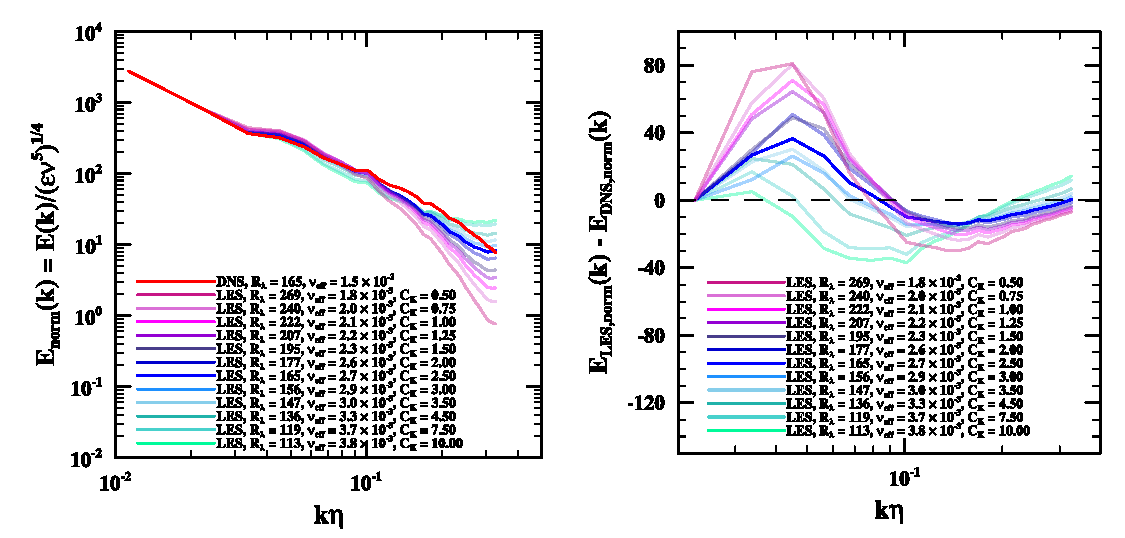
\includegraphics[width=13.5cm]{img/plots/C-sgsspec.pdf}
\caption{
The normalised energy spectra of background turbulent flows for LES depending on subgrid-scale model parameter $C_K$. 
On the left respective spectra are shown with reference DNS spectrum shown in red.
On the right, for more clarity, plot of differences between respective LES spectra and reference DNS spectrum is presented (in log-linear scale).
Spectrum for LES used in this thesis (for $C_K=2.5$) is marked with bolder, more vivid shade of blue.
}
\label{fig:sgsspec}
\end{figure}

Figure \ref{fig:sgsspec} shows energy spectra for LES with different values of $C_K$ and part of the energy spectrum (for $k < k_c = 30$) for the flow generated using DNS (in red) taken as a~reference (left).
On the right, the plot of difference between respective LES spectra with DNS spectrum was produced for more clarity.
In all cases we see characteristic for LES slight overestimation of spectrum for higher wavenumbers and underestimation for intermediate wavenumbers (see Section \ref{ssc:ch2.flow.spec}).
The magnitude of such deviations clearly depends on $C_K$.
For large wavenumbers the overestimation of energy spectrum increases with smaller values of $C_K$ and becomes very high for $C_K < 2$.
On the other hand, for large values of $C_K$ (larger than $4$) such increase is limited for only few highest wavenumbers, and then the spectrum is underestimated for almost entire range of affected modes.
There seems to be range of values of $C_K$ (between $2$ and $4$) where discrepancies in both small and intermediate wavenumbers are balanced out and acceptable throughout entire range of scales considered.
From that range, for the sake of continuity with previous studies, value of $C_K=2.5$ was chosen here to be used in all LES.


\subsubsection{Effective Flow Statistics for LES}

The fact that numerical viscosity in LES is adjusted by spectral-eddy viscosity of the model is the source of another conceptual difficulty.
The majority of derived turbulence statistics used with DNS (see Section \ref{ssc:ch2.flow.bstat}) are calculated using the value of numerical viscosity $\nu$ that parameterises such simulation.
In DNS this is fixed scalar value, but when we include contribution from subgrid-scale model in LES, the effectively used value of viscosity $\nu + \nu_{e}(k|k_c)$ is a nonlinear function of wavenumber $k$.

For that reason, there is an open question how to treat such dependence on viscosity for these statistics.
The approaches vary between authors.
\textcite[Table 1]{Yang2008} do not provide any values directly dependent on $\nu$ for LES.
Some more statistics are presented in \textcite[Table 1]{Jin2010} due to the concept of effective viscosity (see below) but some caution is exerted as value of $R_{\lambda}$ for LES is not specified.
On the other hand, in \textcite[Table 1]{Rosa2017} full comparison of statistics for DNS and LES is provided, including values of $R_{\lambda}$.
In this study, the comparison of collisional particle statistics obtained by DNS and LES is the main goal, and they are dependent on $R_{\lambda}$.
Thus, in this study we present all respective statistics for LES to make comparison more complete, although approximate character of these should be taken into account.
For LES, the effective values of statistics are used, as derived in \textcite{Jin2010}.

In particular, we eliminate spectral-eddy viscosity dependence on $k$ by calculating \emph{average viscosity contribution of subgrid-scale model}, $\bar{\nu}_{\text{SGS}}$ as follows \parencite[Equation 13]{Jin2010}:
\begin{equation}
\bar{\nu}_{\text{SGS}} =
\frac
{\int_{k_0}^{k_c} \nu_{e}(k|k_c) 2 k^2 E(k) dk}
{\int_{k_0}^{k_c} 2 k^2 E(k) dk} ,
\label{egn:rnu-sgs}
\end{equation}
where $E(k)$ is the energy spectrum and $\nu_{e}(k|k_c)$ is defined by Equation \ref{eqn:sgs-1}.
This way we can define SGS-adjusted, or effective, viscosity as: $\nu_{\text{eff}} = \nu + \bar{\nu}_{\text{SGS}}$.
For completeness, we assume that in DNS $\bar{\nu}_{\text{SGS}} \equiv 0$ so that $\nu_{\text{eff}} = \nu$.
Now, we may calculate effective counterparts to flow statistics by replacing $\nu$ with $\nu_{\text{eff}}$ in their definitions.
For example, consider the Kolmogorov length scale, $\eta$, and its effective equivalent:
$$
\eta = \left( \frac{\nu^3}{\epsilon} \right)^{1/4} , \quad \quad \eta_{\text{eff}} = \left( \frac{\nu_{\text{eff}}^3}{\epsilon} \right)^{1/4} = \left( \frac{(\nu + \bar{\nu}_{\text{SGS}})^3}{\epsilon} \right)^{1/4} .
$$

\begin{table}[h]
\centering
\scriptsize
\begin{tabular}{llllllllllllll}
$\mathbf{C_K}$ & \textbf{DNS}* & $0.50$ & $0.75$ & $1.00$ & $1.25$ & $1.50$ & $2.00$ & $\mathbf{2.50}$ & $3.00$ & $3.50$ & $4.50$ & $7.50$ & $10.00$ \\ \hline

$\bar{\nu}_{\text{SGS}} \cdot 10^3$ & --- & 0.31 & 0.46 & 0.60 & 0.72 & 0.84 & 1.07 & \textbf{1.24} & 1.38 & 1.54 & 1.78 & 2.17 & 2.35 \\
$\nu_{\text{eff}}  \cdot 10^3$ & \textbf{1.50} & 1.81 & 1.96 & 2.10 & 2.22 & 2.34 & 2.57 & \textbf{2.74} & 2.88 & 3.04 & 3.28 & 3.67 & 3.85 \\

$u'$ & \textbf{0.87} & 0.85 & 0.86 & 0.86 & 0.86 & 0.86 & 0.86 & \textbf{0.86} & 0.86 & 0.86 & 0.86 & 0.85 & 0.85 \\

$\epsilon$ & \textbf{0.21} & 0.06 & 0.07 & 0.08 & 0.09 & 0.09 & 0.10 & \textbf{0.11} & 0.12 & 0.12 & 0.13 & 0.15 & 0.16 \\
$\epsilon_{\text{eff}}$ & \textbf{0.21} & 0.07 & 0.09 & 0.11 & 0.13 & 0.14 & 0.18 & \textbf{0.20 } & 0.22 & 0.25 & 0.29 & 0.37 & 0.40 \\ \hline

$\eta \cdot 10^2$ & \textbf{1.13} & 1.54 & 1.47 & 1.44 & 1.41 & 1.38 & 1.34 & \textbf{1.32} & 1.31 & 1.29 & 1.26 & 1.23 & 1.21 \\
$\eta_{\text{eff}} \cdot 10^2$ & \textbf{1.13} & 1.77 & 1.80 & 1.84 & 1.89 & 1.93 & 2.01 & \textbf{2.08} & 2.14 & 2.19 & 2.26 & 2.39 & 2.45 \\

$\tau_k \cdot 10^1$ & \textbf{0.84} & 1.58 & 1.45 & 1.38 & 1.32 & 1.28 & 1.21 & \textbf{1.17} & 1.14 & 1.10 & 1.06 & 1.00 & 0.98 \\
$\tau_{k, \text{eff}} \cdot 10^1$ & \textbf{0.84} & 1.74 & 1.65 & 1.62 & 1.60 & 1.60 & 1.57 & \textbf{1.58} & 1.58 & 1.57 & 1.56 & 1.56 & 1.56 \\ \hline

$L_s$ & \textbf{1.46} & 1.54 & 1.52 & 1.51 & 1.51 & 1.51 & 1.50 & \textbf{1.50} & 1.51 & 1.50 & 1.50 & 1.52 & 1.52 \\
$T_e$ & \textbf{3.62} & 12.17 & 10.32 & 9.38 & 8.67 & 8.11 & 7.25 & \textbf{6.77} & 6.44 & 6.02 & 5.55 & 4.89  & 4.62 \\
$T_{e, \text{eff}}$ & \textbf{3.62} & 10.06 & 7.87 & 6.70 & 5.84 & 5.18 & 4.23 & \textbf{3.70} & 3.34 & 2.96 & 2.53 & 1.99 & 1.79 \\ \hline

$\lambda \cdot 10$ & \textbf{2.86} & 5.25 & 4.82 & 4.59 & 4.42 & 4.27 & 4.04 & \textbf{3.90} & 3.81 & 3.68 & 3.53 & 3.31 & 3.22 \\
$\lambda_{\text{eff}} \cdot 10$ & \textbf{2.86} & 5.72 & 5.49 & 5.41 & 5.36 & 5.32 & 5.26 & \textbf{5.25} & 5.25 & 5.22 & 5.20 & 5.16 & 5.13 \\
$R_{\lambda} \cdot 10^{-2}$ & \textbf{1.66} & 2.97 & 2.76 & 2.64 & 2.54 & 2.46 & 2.33 & \textbf{2.24} & 2.18 & 2.11 & 2.03 & 1.89 & 1.83 \\
$R_{\lambda, \text{eff}} \cdot 10^{-2}$ & \textbf{1.66} & 2.69 & 2.40 & 2.22 & 2.08 & 1.95 & 1.77 & \textbf{1.65} & 1.56 & 1.48 & 1.36 & 1.20 & 1.13 \\ \hline
\end{tabular}
\caption{Raw (not considering effective viscosity $\nu_{\text{eff}}$) and effective statistics (in spectral units) of turbulent flows simulated using LES where different values of $C_K$ parameter in Equation \ref{eqn:sgs-2} were used. All simulations were run with $N=64$, $\nu = 1.5 \times 10^{-3}$, $\Delta t = 9 \times 10^{-4}$, and using deterministic forcing scheme. Uncertainties of presented values were omitted for clarity, and are similar to corresponding values in Table \ref{tab:flow-stats}. Column in bold, for $C_K=2.5$ refers to simulation used as LES background flow in actual study. * -- statistics for respective DNS are shown for comparison.
}
\label{tab:sgs-stats}
\end{table}

To provide bigger picture, Table \ref{tab:sgs-stats} shows flow statistics calculated for LES with different subgrid-scale model parameters $C_K$ (and DNS statistics for comparison).
Statistics of flows used in this study (DNS and LES with $C_K=2.5$) are marked in bold.
For additional comparison, values of flow statistics are listed in both ''standard'' and effective versions, so that influence of viscosity contribution of subgrid-scale model may be followed.
Interestingly enough, for many key statistics, such as $\epsilon$ and $R_{\lambda}$, effective values for $C_K=2.5$ are closest to these obtained in DNS, even though the choice of that parameter was made only on the basis of comparison of the energy spectra.
Also note that Kolmogorov scale parameters ($\eta$,~$\tau_k$) decrease with increasing $C_K$ and may be assumed to asymptotically approach values for DNS.

The more troubling observation concerns values of $R_{\lambda}$ (both ''standard'' and effective), which seem to be very sensitive to the choice of $C_K$.
The choice of $C_K$ based on the analysis of energy spectra differences admitted some room for acceptable values of $C_K$ ranging from $2$ to $4$.
Still, $R_{\lambda}$ for simulations within that range may differ by up to $20\%$.
This observation may confirm reservation on part of \textcite{Yang2008} and \textcite{Jin2010}, where it was not explicitly listed.
This matter clearly requires further investigation.
Still, we use effective value of $R_{\lambda}$ for LES simulations, but it must be interpreted with utmost caution.  



\chapter{Super-Particle Parameterisations in Simulations under Two-Way Momentum Coupling}
\label{app:spp}

This appendix serves as a technical reference for simulations under two-way momentum coupling.
It is specified where exactly super-particle parameterisation was used and with what exactly value of parameter $M$, i.e. the ratio between effective number of physical particles and actual number of individually tracked computational particles.
In addition, tables presented here provide cross-reference between the effective number of particles and the particle mass loading for simulations referred to be either of these measures of particle amount.
Note that LES requires higher values of $M$, since setup used in this study did not allow to effectively perform simulations with more than 5 million computational particles (as opposed to DNS, where 10 or 20 million particles were perfectly manageable).
Also, for more information on the impact of super-particle parameterisation on the accuracy of collisional statistics of particles, please refer to brief analysis in \textcite{Rosa2022}.  

\begin{table}[h]
\centering
\scriptsize
\begin{tabular}{l|rr|rr|rr|rr|rr}
\multicolumn{11}{c}{\textbf{DNS}} \\ \hline
& \multicolumn{2}{c|}{$20$~$\upmu\text{m}$} & \multicolumn{2}{c|}{$30$~$\upmu\text{m}$} & \multicolumn{2}{c|}{$40$~$\upmu\text{m}$} & \multicolumn{2}{c|}{$50$~$\upmu\text{m}$} & \multicolumn{2}{c}{$60$~$\upmu\text{m}$} \\
$\mathbf{\Phi_m}$ & $N_{\text{part}}$ & $M$ & $N_{\text{part}}$ & $M$ & $N_{\text{part}}$ & $M$ & $N_{\text{part}}$ & $M$ & $N_{\text{part}}$ & $M$ \\ \hline
0.01 & 10.789 & 1 & 3.197 & 1 & 1.349 & 1 & 0.691 & 1 & 0.400 & 1 \\ 
0.05 & 53.945 & 5 & 15.984 & 2 & 6.743 & 1 & 3.453 & 1 & 1.998 & 1 \\ 
0.10 & 107.891 & 10 & 31.968 & 4 & 13.486 & 2 & 6.905 & 1 & 3.996 & 1 \\ 
0.50 & 539.453 & 50 & 159.838 & 20 & 67.432 & 10 & 34.525 & 4 & 19.980 & 2 \\  
1.00 & 1 078.906 & 100 & 319.676 & 40 & 134.863 & 20 & 69.050 & 8 & 39.959 & 4 \\ \hline 
%\multicolumn{11}{c}{}\\ 
%\multicolumn{11}{c}{\textbf{LES}} \\ \hline
%& \multicolumn{2}{c|}{$\mathbf{20 \; \mu \text{m}}$} & \multicolumn{2}{c|}{$\mathbf{30 \; \mu \text{m}}$} & \multicolumn{2}{c|}{$\mathbf{40 \; \mu \text{m}}$} & \multicolumn{2}{c|}{$\mathbf{50 \; \mu \text{m}}$} & \multicolumn{2}{c}{$\mathbf{60 \; \mu \text{m}}$} \\
%$\mathbf{\Phi_m}$ & $N_{\text{part}}$ & $M$ & $N_{\text{part}}$ & $M$ & $N_{\text{part}}$ & $M$ & $N_{\text{part}}$ & $M$ & $N_{\text{part}}$ & $M$ \\ \hline
%0.01 & 6.630 & 2 & 1.964 & 1 & 0.829 & 1 & 0.424 & 1 & 0.246 & 1 \\ 
%0.05 & 33.149 & 7 & 9.822 & 2 & 4.144 & 1 & 2.121 & 1 & 1.228 & 1 \\ 
%0.10 & 66.297 & 14 & 19.644 & 4 & 8.287 & 2 & 4.243 & 1 & 2.455 & 1 \\ 
%0.50 & 331.487 & 70 & 98.218 & 20 & 41.436 & 10 & 21.215 & 5 & 12.277 & 3 \\  
%1.00 & 662.974 & 135 & 196.437 & 40 & 82.872 & 18 & 42.430 & 10 & 24.555 & 5 \\ \hline 
\end{tabular}
\caption{Super-particle factors ($M$) and approximate effective number of particles in millions ($N_{\text{part}}$) for DNS simulations used in plots depending on particle radius ($a$) and for fixed values of the particle mass loading ($\Phi_m$).
The values of $M$ for LES are, in general, equal to twice the value shown for DNS (except when $N_{\text{part}} < 5 \, \text{million}$, where $M=1$).
}
\label{tab:spp-phic}
\end{table}

Table \ref{tab:spp-phic} shows values of $M$ used in simulations for plotting statistics dependent on particle radius for certain fixed values of $\Phi_m$, such as in Figures \ref{fig:twcrdf}, \ref{fig:twcrrv}, and \ref{fig:twcgamma} (top plots).
Note, that attaining high mass loadings ($\Phi_m = 1$) for simulations with the smallest particles considered ($a = 20$~$\upmu\text{m}$) requires simulation to contain over 1 billion of particles, which is hardly viable.
Thus, such simulations had to be performed using relatively high values of $M$, which might have influenced results more than in other cases, and it needs to be kept in mind.

\begin{table}[h]
\centering
\scriptsize
\begin{tabular}{lrrrrrrrrrrr}
$N_{\text{part}}$ [millions] & 1 & 2 & 3 & 4 & 5 & 6 & 8 & 10 & 12 & 15 & 20 \\ \hline
$\Phi_m$ [$a = 30$~$\upmu\text{m}$] & 0.003 & 0.006 & 0.009 & 0.013 & 0.016 & 0.019 & 0.025 & 0.31 & 0.038 & 0.047 & 0.063 \\
$\Phi_m$ [$a = 40$~$\upmu\text{m}$] & 0.007 & 0.015 & 0.022 & 0.030 & 0.037 & 0.044 & 0.059 & 0.074 & 0.089 & 0.111 & 0.148 \\
$M$ [LES only] & 1 & 1 & 1 & 1 & 1 & 2 & 2 & 2 & 3 & 3 & 4 \\
\end{tabular}
\caption{Respective particle mass loadings ($\Phi_m$) for simulations with smaller amount of particles (up to 20 million) for $a = 30$, $40$~$\upmu\text{m}$.
Bottom row list necessary values of $M$ used for super-particle parameterisation in LES.
}
\label{tab:spp-base}
\end{table}

Tables \ref{tab:spp-base} and \ref{tab:spp-ext} provide association between effective number of particles and respective mass loadings in simulations used for plotting values depending on amount of particles of radii $30$~$\upmu\text{m}$ and $40$~$\upmu\text{m}$ in the system.
These refer to plots for smaller amounts of particles (up to 20 million, see Figures \ref{fig:twcrdf}, \ref{fig:twcrrv}, and \ref{fig:twcgamma}; bottom plots) and for higher mass loadings as well in log scale (see Figures \ref{fig:twcrdfext}, \ref{fig:twcrrvext}, and \ref{fig:twcgammaext}).

\begin{table}[h]
\centering
\scriptsize
\begin{tabular}{lrrrrrrrrrrrrrr}
$N_{\text{part}}$ [millions] & 30 & 40 & 60 & 80 & 100 & 120 & 140 & 160 & 180 & 200 & 250 & 300 & 350 & 400 \\ \hline
$\Phi_m$ [$a = 30$~$\upmu\text{m}$] & 0.09 & 0.13 & 0.19 & 0.25 & 0.31 & 0.38 & 0.44 & 0.50 & 0.56 & 0.63 & 0.78 & 0.94 & 1.09 & 1.25 \\
$\Phi_m$ [$a = 40$~$\upmu\text{m}$] & 0.22 & 0.30 & 0.44 & 0.59 & 0.74 & 0.89 & 1.04 & 1.19 & 1.33 & 1.48 & 1.85 & 2.22 & 2.60 & 2.97 \\
\end{tabular}
\caption{Respective particle mass loadings ($\Phi_m$) for simulations with larger number of particles (higher than 20 million) for $30$, $40$~$\upmu\text{m}$.
}
\label{tab:spp-ext}
\end{table}


For DNS, all simulations up to 20 million particles were performed without super-particle parameterisation.
For larger $N_{\text{part}}$, simulations with 10 million computation particles were used, where $M$ was set to value given by target effective number of particles divided by 10~million, up to $M = 40$ for simulations with 400 million particles.
Similar approach was used for LES, but due to technical limitations largest workable amount of computational particles tracked was limited to 5 million.
For that reason, simulations with number of particles between 6 and 20 million also required super-particle parameterisation, with small values of $M$, as listed in Table \ref{tab:spp-base}.
For values larger than 20 million simulations with 5 million computational particles were employed, thus resulting in two times larger values of $M$ than in DNS for the same target number of particles (up to $M=80$ for simulation with 400 million effective particles).








\addcontentsline{toc}{chapter}{\numberline{}References}
\printbibliography[title=References]

\end{document}
